
\pdfminorversion=4
\documentclass[letterpaper,12pt]{article}
\usepackage[top=1in, bottom=1in, left=1.25in, right=1.25in]{geometry}
\usepackage{setspace}
\setcounter{secnumdepth}{3} % this number depends on your depth of sections
\setcounter{tocdepth}{3} % this number should be equal to secnumdepth in previous
\usepackage{subfigure}
\usepackage[subfigure]{tocloft}
\renewcommand\cftloftitlefont{\normalsize\bfseries}
\renewcommand\cftlottitlefont{\normalsize\bfseries}
\usepackage{tocstyle}
\renewcommand{\contentsname}{\centerline {\normalsize\bfseries Table of Contents}}
\newtocstyle[standard][leaders]{mytocstyle}{\settocfeature[1]{entryhook}{\normalfont\bfseries}}

\usetocstyle{mytocstyle}
\usepackage{sectsty}
\sectionfont{\normalsize\centering}
\subsectionfont{\normalsize}
\usepackage{enumitem}
\renewcommand{\thesection}{}
\renewcommand{\thesubsection}{\arabic{section}.\arabic{subsection}}
\usepackage{algorithmicx}
\usepackage{algorithm}
\usepackage{algpseudocode}
\usepackage{algpascal}
\usepackage{algc}
\usepackage{graphicx}
\usepackage{times}
\usepackage{latexsym}
\usepackage{graphicx}
\usepackage{subfigure}
\usepackage{cite}
\usepackage{balance}
\usepackage{multirow}
\usepackage{epstopdf}
\usepackage{threeparttable}
\usepackage[latin1]{inputenc}
\usepackage{amsmath}
\usepackage{amsfonts}
\usepackage{amssymb}
\usepackage{amsthm}
%\usepackage{algorithm}
%\usepackage{algorithmic}
\graphicspath{ {images/} }
\usepackage{graphicx}
\usepackage{comment}
\usepackage{times}
\usepackage{cite}
\newtheorem{theorem}{Theorem}
\newtheorem{lemma}{Lemma}
\newtheorem{definition}{Definition}
\newenvironment{alginc}[1][pseudocode]{\medskip\algsetlanguage{#1}\begin{algorithmic}[1]}{\end{algorithmic}\medskip}
\newcommand{\Exp}{Exponential }
\newcommand{\G}{\mathbb{G}}
\newcommand{\Z}{\mathbb{Z}}
\newcommand{\PP}{Pairing }
\newcommand{\Gone}{\mathbb{G}_1}
\newcommand{\Gtwo}{\mathbb{G}_2}
\newcommand{\Gthree}{\mathbb{G}_3}
\newcommand{\Gt}{\mathbb{G}_T}
\newcommand{\PPo}{Pairing}

\usepackage[colorlinks=true,linkcolor=black,citecolor=red,urlcolor=red,plainpages=false,pdfpagelabels=true, bookmarks=false]{hyperref}
\begin{document}
   \author{{\normalsize Chunqiang Hu}}
   \title{\Large{\bf Privacy-Preserving and Secure Cryptographic Schemes for Wireless Applications} \\ \large Dissertation Proposal}
   \date{}
   \maketitle
   \thispagestyle{empty}
   \begin{center}
       B.S. in Computer Science and Technology,\\ May 2006, Southwest University \\
       M.S. in Computer Applications and Technology,\\ May 2009, Chongqing University \\
       A Dissertation Proposal submitted to\\[\baselineskip]
       The Faculty of\\The School of Engineering and Applied Science\\ of The George
       Washington University\\ in partial satisfaction of the requirements\\ for the degree
       of Doctor of Philosophy\\[\baselineskip]
       April 24, 2015\\[\baselineskip]
       Dissertation directed by\\[\baselineskip]
       Xiuzhen Cheng\\Professor of Computer Science
   \end{center}
   % display page numbers in the footer and centered. Start with roman numerals %
   \pagestyle{plain}
   \setcounter{page}{1}
   \pagenumbering{roman}



   \newpage
   \doublespacing
   \begin{center}
   {\Large{\bf Privacy-Preserving and Secure Cryptographic Schemes for Wireless Applications }\\ \large Dissertation Proposal}\\[\baselineskip]
   {\normalsize Chunqiang Hu}
   \end{center}
   \noindent Dissertation Proposal Committee:\\

   \hfill\begin{minipage}{5in}
   {Xiuzhen Cheng, Professor of Computer Science, Dissertation
       Director}\\[\baselineskip]
   {Hyeong-Ah Choi, Professor of Computer Science, Committee Member}\\[\baselineskip]
   {Nan Zhang, Associate Professor of Computer Science, Committee Member}\\[\baselineskip]
   {Hang Liu, Associate Professor of Electrical and Computer Engineering, Committee Member}\\[\baselineskip]
   \end{minipage}

   \newpage
      \section{Abstract}
    Many applications based on wireless technologies become very popular in real world, such as smart grids, social networks, body area networks (BANs), electric vehicle (EV) etc.  The wireless applications have gained tremendous attention among researchers and engineers as they have new features such as demand-response, multicast communications, or billing purpose. Despite these attractive features, the wireless applications also exist many challenges, especially in data security and privacy.  Security and privacy issues are crucial in almost wireless applications. How to protect the user's data security and privacy to meet the requirement of certain wireless applications? It is a challenge problem.

      In this dissertation proposal, we target to protect data security and privacy in wireless applications by cryptographic mechanisms as follows.

      First, I consider a special type of multicast communications existing in many emerging applications such as smart grids, social networks, and body area networks, in which the multicast destinations are specified by an access structure defined by the data source based on a set of attributes and carried by the multicast message. A challenging issue is to secure these multicast communications to address the prevalent security and privacy concerns, i.e., to provide access control, data encryption, and authentication to ensure message integrity and confidentiality. To achieve this objective, we present a signcryption scheme called CP\_ABSC based on Ciphertext-Policy Attribute Based Encryption (CP\_ABE). CP\_ABSC provides algorithms for key management, signcryption, and designcryption. It can be used to signcrypt a message/data based on the access rights specified by the message/data itself. A multicast destination can designcrypt a ciphertext if and only if it possesses the attributes required by the access structure of the data. Thus CP\_ABSC effectively defines a multicast group based on the access rights of the data.   CP\_ABSC provides collusion attack resistance, message authentication, forgery prevention, and confidentiality. It can be easily applied to secure the push-based multicast from the data source to multiple destinations and the data retrieval from a repository by multiple destinations (pull-based multicast). Compared to CP\_ABE, CP\_ABSC combines encryption with signature at a lower computational cost for signcryption and a slightly higher cost in designcryption for signature verification.

      Second, many applications can be modeled by a simple client-server architecture, however, achieving privacy protection at the client side is a non-trial problem as payment for the services must be computed by the server at the end of each billing period. We propose a privacy preservation and billing scheme termed PPDIR based on delayed information release. PPDIR relies on a novel group signature mechanism and the asymmetric Rabin cryptosystem to protect the privacy of the clients and their requests, to achieve accountability and non-repudiation, and to shift the computational complexity to the server side. It adopts a secret token for anonymity and the token is updated for each client at the beginning of each billing period and securely released to the server at the end of the billing period. Such a strategy can prevent the server from linking a client's requests made at different billing periods.  It also prevents any adversary from linking any request to any client. Note that the server is able to figure out all requests made by a client within a billing period after receiving the delayed token, which is unavoidable for billing purpose. We prove the security properties of the group signature scheme, and analyze the security strength of PPDIR. Our study indicates that PPDIR can achieve privacy-preservation, confidentiality, non-repudiation, accountability, and other security properties. We also evaluate the performance of our scheme in terms of communicational and computational overheads.

      Third, in emerging applications such as e-healthcare, the patient protects personalized medicine and patient similarity, there is often a need to specify a access policy in the ciphertext and only individuals who satisfy the policy can decrypt. More generally, we may want to only give access to a function of the plaintext, depending on the decryptor's authorization. Function encryption can solve the problem, however function encryption is an abstract concept, how to design the specific functional encryption to solve the problem, it is challenge problem. I will focus my attention to design the specific functional encryption to meet the requirement of applications.
      \newpage

   \newgeometry{top=1in, bottom=1in, left=1.125in, right=1.125in}
   \tableofcontents
   \restoregeometry
   \newpage


   \cleardoublepage
   \phantomsection \label{listoffig}
   \addcontentsline{toc}{section}{\hspace{1.5pt} List of Figures}
   \begin{center}
       \listoffigures
   \end{center}
   \newpage


   \newpage
   \setcounter{page}{1}
   \setcounter{section}{1}
   \pagenumbering{arabic}
   \begin{singlespace}
       \section{Introduction}
   \end{singlespace}
   \setcounter{section}{1}
   \doublespacing
Many applications based on wireless technologies become very popular in real world, such as smart grids, social networks, body area networks (BANs), electric vehicle (EV) etc.  The wireless applications have gained tremendous attention among researchers and engineers as they have new features such as demand-response, multicast communications, or billing purpose. Despite these attractive features, the wireless applications also exist many challenges, especially in data security and privacy \cite{rial2011privacy, popa2009vpriv, jorns2007privacy, ma2013privacy, erkin2012private, lagendijk2013encrypted, anderson2010security, buttyan2007security, hu2013body, su2009ocast}. It is crucial to solve security and privacy issues in almost wireless applications. We will introduce the challenges of security and privacy from three angles as follows:

%\noindent{\bf Multicast communications}

\subsection{Multicast communications}

We consider a special type of multicast communications existing in emerging applications such as smart grids, social networks, and body area networks:  a multicast message carries an access structure specified by the data source based on a set of attributes to define the right set of destinations - a recipient of the message can read the data only if it possesses the set of attributes required by the data source via the access structure. Such multicasts are very popular in many applications. For example, in smart metering, a service provider can broadcast a software update command to the smart meters of model A or B located at a certain area manufactured by company X after 2010 (\emph{push-based} multicast) and the message carries an access structure defined by attributes \{location, time, company, model\} based on the  AND and OR relations; a smart meter readings together with its access policy (only the service providers in Washington DC or Bethesda MD can access this data), again defined by AND and OR relations, can be stored in a data repository for future downloads by all the service providers in Washington DC or Bethesda MD (\emph{pull-based} multicast).

The push-based multicast under our consideration is very similar to the traditional ones except that no identities of the destinations are carried by the message; pull-based multicasts require the data to be stored in a repository and then downloaded by multiple users on-demand. Both multicast scenarios require the data to be protected for confidentiality, integrity, authentication, and access control. Specifically,
\begin{itemize}
\item All the multicast messages from the data source should be protected from adversaries as the data may disclose private information of the data source. For example, the electricity usage data could reveal the activities of the residents in a household \cite{Hart92}, which places a significant privacy concern.
\item The data source should provide access control and intelligently determine who should or should not have access to its data. An access structure should be defined based on the attributes required by the data source. The data should be accessible only by the destinations specified by the data source; no third party including the data repository should be able to read the data.
\item The authenticity of the data source and the integrity of the data should be verifiable.
\end{itemize}

To achieve these objectives, we propose a signcryption scheme termed CP\_ABSC based on Ciphertext-Policy Attribute-based Encryption (CP\_ABE) \cite{bethencourt2007ciphertext} to address the secure multicast problem and provide the required security services mentioned above. CP\_ABSC combines signature and encryption, and provides a new mechanism for data encryption, access control, and authentication to ensure security and privacy. The basic idea of CP\_ABSC is to signcrypt a data item based on its access policy (represented by an access tree and specified by the data (data source) itself) and designcrypt the corresponding ciphertext with a secret key computed from a set of attributes. The access tree defines the access rights of the data based on the attributes and is carried by the ciphertext. This implies that any user possessing the set of attributes that satisfy the access policy defined by the data itself can access the data. Because a multicast group is uniquely defined by the data itself via the access policy, secure multicasts are effectively achieved. Moreover, other than supporting the traditional push-based multicast that ``pushes'' the data to all destinations, CP\_ABSC can also support pull-based multicast, in which the data is stored in a repository and delivered to a multicast destination only when the destination needs the data and actively ``pulls'' the data. The detailed scheme is introduced in the Section 3.

\subsection {Privacy Preservation Scheme}

Many real world applications can be modeled with a simple client-server architecture, in which clients send requests to the server and get services from the server on demand. For example, location based services (LBS) allow mobile users to contact LBS servers via their smart devices to get context information such as the closest gas station or the most highly rated Asia restaurant within 5 miles. Smart metering can also be regarded as following this simple client-server model as smart meters (clients) periodically report the fine-grained electricity usage data to utility companies (servers), though the utility company does not have to respond to each report (a null response from the server). Such applications share the following properties:
\begin{itemize}
\item The data (a LBS request or a smart meter reading) sent from a client to the server can reveal the private information of the client. For examples, LBS requests could be exploited to trace a mobile user and infer the user's private information such as race and age as the request contents contain the location and preferences of the user; smart meter readings can be explored to figure out the presence/absence and habit of a residence as the fine-grained utility data closely reflect the activities of the residence. Such a privacy disclosure triggers many security and safety concerns, and even physical attacks to the clients.
\item Protecting the privacy of the clients and the confidentiality of the requests can be achieved via traditional and advanced cryptographic primitives but unfortunately existing research exhibits the following disadvantages of such approaches:  (i) the computational overhead is prohibitively high as in general advanced crypto tools such as homomorphic encryption is employed but the client devices in our application scenarios are typically relatively ``dumb'' (smart phones, smart meters, etc.); (ii) completely hiding the clients via anonymous communications to prevent the server and adversaries from linking the requests made by the same client renders the traditional billing impossible, which causes further security problems; (iii) many proposed approaches such as privacy-preserving data aggregation for smart metering actually could not achieve the desired objectives as the coarse-grained aggregated data gets rid of the advantages provided by fine-grained utility data for smart grid services, which implies a sacrifice of service with privacy protection.
\end{itemize}

These observations motivate us to study the following novel problem under a simple client-server model: \emph{how to protect the privacy of the clients while simultaneously getting services from the server and paying the server for the received services in a billing period?} This is a non-trivial problem as our design has to consider the following security challenges and objectives:
\begin{itemize}
\item All the requests from the clients should be protected from adversaries as the request content may disclose private information. The requests made by the same client should be unlinkable to the adversaries; the requests made by the same client in different billing periods should be unlinkable to the server.
\item A client should never be able to deny the requests/services it has made/received and the server should never be able to forge a service not requested by any client without being detected. The privacy preservation scheme must be accountable.
\item The computational overhead at the client side should be small.
\end{itemize}

To tackle these challenges, we propose a novel accountable scheme to provide \underbar{\bf{P}}rivacy \underbar{\bf{P}}reservation and billing via \underbar{\bf{D}}elayed \underbar{\bf{I}}nformation \underbar{\bf{R}}elease (PPDIR) for client-server based applications. PPDIR employs (i) a novel group signature scheme such that the signature of each client request is verifiable (the request is from a legitimate client) but the server is not able to figure out who the client is without further information; (ii) the asymmetric Rabin's public-key cryptosystem to encrypt the request with the server's public key to provide request confidentiality; (iii) AES to protect the server responses; and (iv) a one-way hash chain seeded by a token that changes at the beginning of each billing period such that the server can link the requests made by the same client when the token is securely released to the server at the end of the current billing period but no one can link the requests from different billing periods. We carry out a rigorous analysis to investigate the security properties of the proposed group signature mechanism, and the security strength and computational/communication overhead of PPDIR. Section 4 gives the detailed description.

\subsection{Advance Privacy Preservation Scheme}

For many emerging applications such as cloud services this notion of public-key encryption is insufficient. For example, there is often a need to specify a decryption policy in the ciphertext and only individuals who satisfy the policy can decrypt. More generally, we may want to only give access to a function of the plaintext, depending on the decryptor's authorization. As a concrete example, consider a cloud service storing encrypted images. Law enforcement may require the cloud to search for images containing a particular face. Thus, the cloud needs a restricted secret key that decrypts images that contain the target face, but reveals nothing about other images. More generally, the secret key may only reveal a function of the plaintext image, for example an image that is blurred everywhere except for the target face. Traditional public-key cryptography cannot help with such tasks.

Function encryption can solve the problem, however function encryption is an abstract concept, how to design the specific functional encryption to solve the problem, it is challenge problem. I will focus my attention to design the specific functional encryption to meet the requirement of applications.
%
%The remainder of this section is structured as follows: In Section \ref{sec:motivation}, we presents the motivations and our system model, and summarize the most related work. Section \ref{sec:CP-ABSC} proposes our signcryption scheme CP\_ABSC and illustrates how to use it to secure multicast communications. Section \ref{sec:correctness_performance} proves the correctness of CP\_ABSC and analyzes its security strength and computational cost.    %Section \ref{sec: Integration of attribute based signature} evaluates an attribute based implementation.
%Conclusions and future research are presented in Section \ref{sec:conclusion}.


   \newpage
      \begin{singlespace}
           \section{Preliminaries}
      \end{singlespace}
   \label{preliminaries}
\subsection{Bilinear Mapping and the Bilinear Diffie-Hellman problem}

Let $\mathbb{G}_1$, $\mathbb{G}_2$, and $\mathbb{G}_3$ be three bilinear groups of prime order $p$, and let $g_1$ be a generator of $\mathbb{G}_1$ and $g_2$ be a generator of $\mathbb{G}_2$.  Our
proposed scheme makes use of a bilinear mapping: $e: \mathbb{G}_1\times \mathbb{G}_2\rightarrow \mathbb{G}_3$ with the following properties:

\begin{enumerate}
\item {\em Bilinear:} A mapping $e: \mathbb{G}_1\times \mathbb{G}_2\rightarrow \mathbb{G}_3$ is bilinear if and only if for $\forall P\in \mathbb{G}_1, \forall Q\in \mathbb{G}_2$, and $\forall a, b \in \mathbb{Z}_p$, $e(P^a,Q^b)=e(P,Q)^{ab}$ holds. Here $\mathbb{Z}_p = \{0, 1, \ldots, p-1\}$ is a Galois field of order $p$.
\item {\em Non-degeneracy:} The generators $g_1$ and $g_2$ satisfy $e(g_1,g_2)\neq 1$.
\item {\em Computability:} There is an efficient algorithm to compute $e(P,Q)$ for $\forall Q \in \mathbb{G}_2$.
\end{enumerate}

With a bilinear mapping, one can get the following {\bf Bilinear Diffie-Hellman problem (BDH)}:
 Given three groups $\mathbb{G}_1$, $\mathbb{G}_2$, and $\mathbb{G}_3$ of the same prime order $p$. Let $e: \mathbb{G}_1\times \mathbb{G}_2\rightarrow \mathbb{G}_3$ be a bilinear mapping and $g_1$, $g_2$ be respectively the generators of $\mathbb{G}_1$ and $\mathbb{G}_2$. The objective of BDH is to compute $e(g_1,g_2)^{abc}$, where $a,b,c\in \mathbb{Z}_p$, from the given $(g_1,g_1^a,g_1^c,g_2,g_2^a,g_2^b)$.

Note that the hardness of the CBDH - i.e., the Computational Bilinear Diffie-Hellman problem (CBDH) - forms the basis for the security of our scheme.


\subsection{Secret Sharing}

Another important cryptographic primitive used by our CP\_ABSC is secret sharing \cite{shamir1979share,HuVMSS12}. In the context of a {\em dealer} sharing a secret with $n$ {\em participants} $u_1, \ldots, u_n$, a participant learns the secret if and only if it can cooperate with at least $t - 1$ other participants (on sharing what they learn from the dealer), where $t \leq n$ is a pre-determined parameter. The secret to be shared by the dealer is $s \in \mathbb{Z}_p$, where $p> n$. Before secret sharing, each participant $u_i$ holds a pairwise secret key $k_i \in \mathbb{Z}_p$, which is only known by $u_i$ and the dealer.

The dealer follows a two-step process. First, it constructs a polynomial function $f(z)$ of degree $t-1$, i.e.,
\begin{equation}
f(z)=s+\sum_{j=1}^{t-1}a_jz^j, \label{equ:fx}
\end{equation}
by randomly choosing $t-1$ i.i.d. coefficients (the $a_j$'s) from $\mathbb{Z}_p$. Note that all (additive and multiplicative) operations used in (\ref{equ:fx}) and throughout the rest of the paper are modular arithmetic (defined over $\mathbb{Z}_p$) as opposed to real arithmetic. Also note that $s$ forms the constant component of $f(z)$ - i.e., $s = f(0)$. Then, in the second step, the dealer transmits to each $u_i$ a secret share $s_i$ computed from $k_i$, the secret key known only by $u_i$ and the dealer.
\begin{align}
s_i = f(k_i),
\end{align}

We now show how $t$ or more users can cooperate to recover $s$ by sharing the secret shares received from the dealer. Without loss of generality, let $u_1, \ldots, u_t$ be the cooperating users. These $t$ users can reconstruct the secret $s = f(0)$ from $s_1 = f(k_1), \ldots, s_t = f(k_t)$ by computing
%
\begin{equation}
s = f(0)=\sum_{j=1}^t \left(s_j \prod_{i \in [1, t],i\neq j}\frac{0-k_{i}}{k_{i}-k_{j}} \right). \label{equ:lac}
\end{equation}

Note that the cumulative product in (\ref{equ:lac}) is essentially a Lagrange coefficient. The correctness of (\ref{equ:lac}) can be
easily verified based on the definition of $f(z)$.

\subsection {Group Signature} \label{sec: IBGS}
Generally speaking,  a group signature scheme \cite{chaum1991group} consists of the following procedures:

\begin{itemize}
\item \emph{Setup}:
A group manager generates a group public key and a group secret key based on certain algorithms.

\item \emph{Join}: The group manager generates a secret key and a public key for a potential user, which might be a new group member.

\item \emph{Sign}: A group member signs its message using its secret key, member certificate, and so on.

\item \emph{Verify}: An algorithm exists to compute the validity of the signature based on the group public key.

\item \emph{Reveal}: Given a signed message and the group secret key, an algorithm (or the group manager) exists to return the identity of the signer.
\end{itemize}

A secure group signature must satisfy the following properties:

\begin{itemize}
\item \emph{Correctness}: Signatures produced by a group member can be accepted by the verifier.

\item \emph{Unforgeability}: Only group members can sign messages on behalf of the group.

\item \emph{Anonymity}: Given a valid signature, it is computationally hard to identify the signer by anyone except the group manager.

\item \emph{Unlinkability}: Whether two different valid signatures are computed by the same group member is computationally hard to figure out by anyone except the group manager.

\item \emph{Exculpability}: Neither the group manager nor a group member can sign messages on behalf of other group members; a member is not responsible for any valid signature that is not produced by itself.
\end{itemize}

\subsection{The Rabin Cryptosystem}
The Rabin cryptosystem \cite{rabin1979digital} is a provably secure public key encryption scheme. Its security strength is based on the practical difficulty of factoring the product of two large prime numbers.

\begin{itemize}
\item \emph{Key Generation}: Each entity needs to create a public key $n$ and the corresponding private key pair $\{n_1, n_2\}$  by finding two large random primes $n_1$ and $n_2$, with roughly the same size, and then setting $n=n_1n_2$. % \emph{A}'s public key is $n$; \emph{A}'s private key is $(n_1, n_2)$.

\item \emph{Encryption}: To send an encrypted message to \emph{A}, \emph{B} encrypts its plaintext $M$ based on \emph{A}'s public key $n$ as follows: \emph{B} treats $M$ as an integer in the range $\{0, 1, 2,..., n-1\}$ and then computes $C=M^2 \mod n$, where $C$ is the ciphertext to be sent to \emph{A}.

\item \emph{Decryption}: The receiver \emph{A} recovers the plaintext $M$ from $C$ based on its private key pair $\{n_1, n_2\}$ according to the following procedure:
\begin{enumerate}
\item   \emph{A} computes $m_1$, $m_2$, $m_3$, and $m_4$ based on the Chinese Remainder Theorem:
\begin{eqnarray}
m_1 & = & C^{(n_1+1)/4} \mod n_1 \nonumber \\
m_2 & = & (n_1-C^{(n_1+1)/4}) \mod n_1 \nonumber \\
m_3 & =& C^{(n_2+1)/4} \mod n_2 \nonumber \\
m_4 & = & (n_2-C^{(n_2+1)/4}) \mod n_2 \nonumber
\end{eqnarray}

\item \emph{A} computes four messages $M_1$, $M_2$, $M_3$, and $M_4$ as follows:
\begin{eqnarray}
M_1 & = & (a m_1+b m_3) \mod n  \nonumber \\
M_2 & = &(a m_1+b m_4) \mod n\nonumber \\
M_3 & = & (a m_2+b m_3) \mod n\nonumber \\
M_4 & = & (a m_2+b m_4) \mod n\nonumber
\end{eqnarray}
where $a=n_2 (n_2^{-1} \mod n_1)$ and $b=n_1 (n_1^{-1} \mod n_2)$.

\item  One of $\{M_1, M_2, M_3, M_4\}$ is the original message $M$. To determine which message is $M$, \emph{B} can add predetermined redundancy before encryption, based on which \emph{A} can figure out the original message $M$.
\end{enumerate}

\end{itemize}


   \newpage
   \begin{singlespace}
   \section{An Attribute-Based Signcryption Scheme to Secure Attribute-Defined Multicast Communications}\label{sec:CP_ABSC_title}
   \end{singlespace}



%===============================================================================

\subsection {Motivations, System Model} \label{sec:motivation}

In this section, we first describe a few real world applications to motivate our problem formulation. Then we present our system model and summarize the most related research.

\subsubsection{Push-based Multicast Communications} \label{sec:push}

Traditional multicast communications are usually \emph{push-based}, in which the data source pushes the data to all recipients (the multicast destinations) whose identities are unique and known to the source ahead of time via one or more simultaneous transmissions. In this study, we consider a variation of the traditional multicast, in which the destinations are defined based on a set of attributes, i.e., the destinations must possess certain attributes in order to receive a multicast message. Such multicasts are popular in emerging applications such as smart grids and social networks. % We describe two real applications to introduce the challenges in the communication mechanism.

Fig.\ref{sec:Fig1:Smart_Grid_Architecture} illustrates a push-based multicast in smart metering, in which a service provider sends instructions or commands to a group of smart meters specified by their locations, models, the connected smart devices, and other attributes. For example, a service provider may broadcast a critical software update message to all smart meters at the Inverness Village whose connected devices include the smart fridges with model number 00000 or 11111 manufactured by XYZ company.  This multicast message does not need to specify the identities of the smart meters (and smart devices); instead, it carries the following access structure defined by AND and OR relations: \emph{Inverness Village AND smart fridges AND manufactured by XYZ company AND (model 00000 OR model 11111)}. Such an access structure clearly specifies the set of destinations that should receive the multicast message - it may not be practical to include a unique identity for each device in the multicast message. A similar scenario is observed in friend discovery in mobile social networks (see Fig.\ref{sec:Fig2:Social_network}), in which a user who wants to make friends with similar interests (reading certain types of novels, traveling to the east coast, enjoying sea food, etc.) broadcasts a query message carrying an access structure that specifies the type of friends the user is looking for.


These applications require a secure push-based multicast that can provide \emph{access control} (not every recipient should be able to access the content of the message), \emph{data encryption} (the query or the instruction should be kept confidential), and \emph{authentication} (the data source should be verifiable and the data integrity should be protected) to ensure message integrity and confidentiality. But unfortunatley push-based multicast authentication schemes such as TELSA, Biba, HORS, and OTS \cite{li2011multicast, neumann2004horse, perrig2001biba, reyzin2002better, wang2009time, perrig2005tesla, kgwadi2011securing} focus on authentication while ignoring access control and confidentiality. Moreover, the multicast destinations in our problem are defined by an access structure specified by the data source, which renders many popular secure multicast protocols inapplicable.

\begin{figure}[!htp]
\centering
 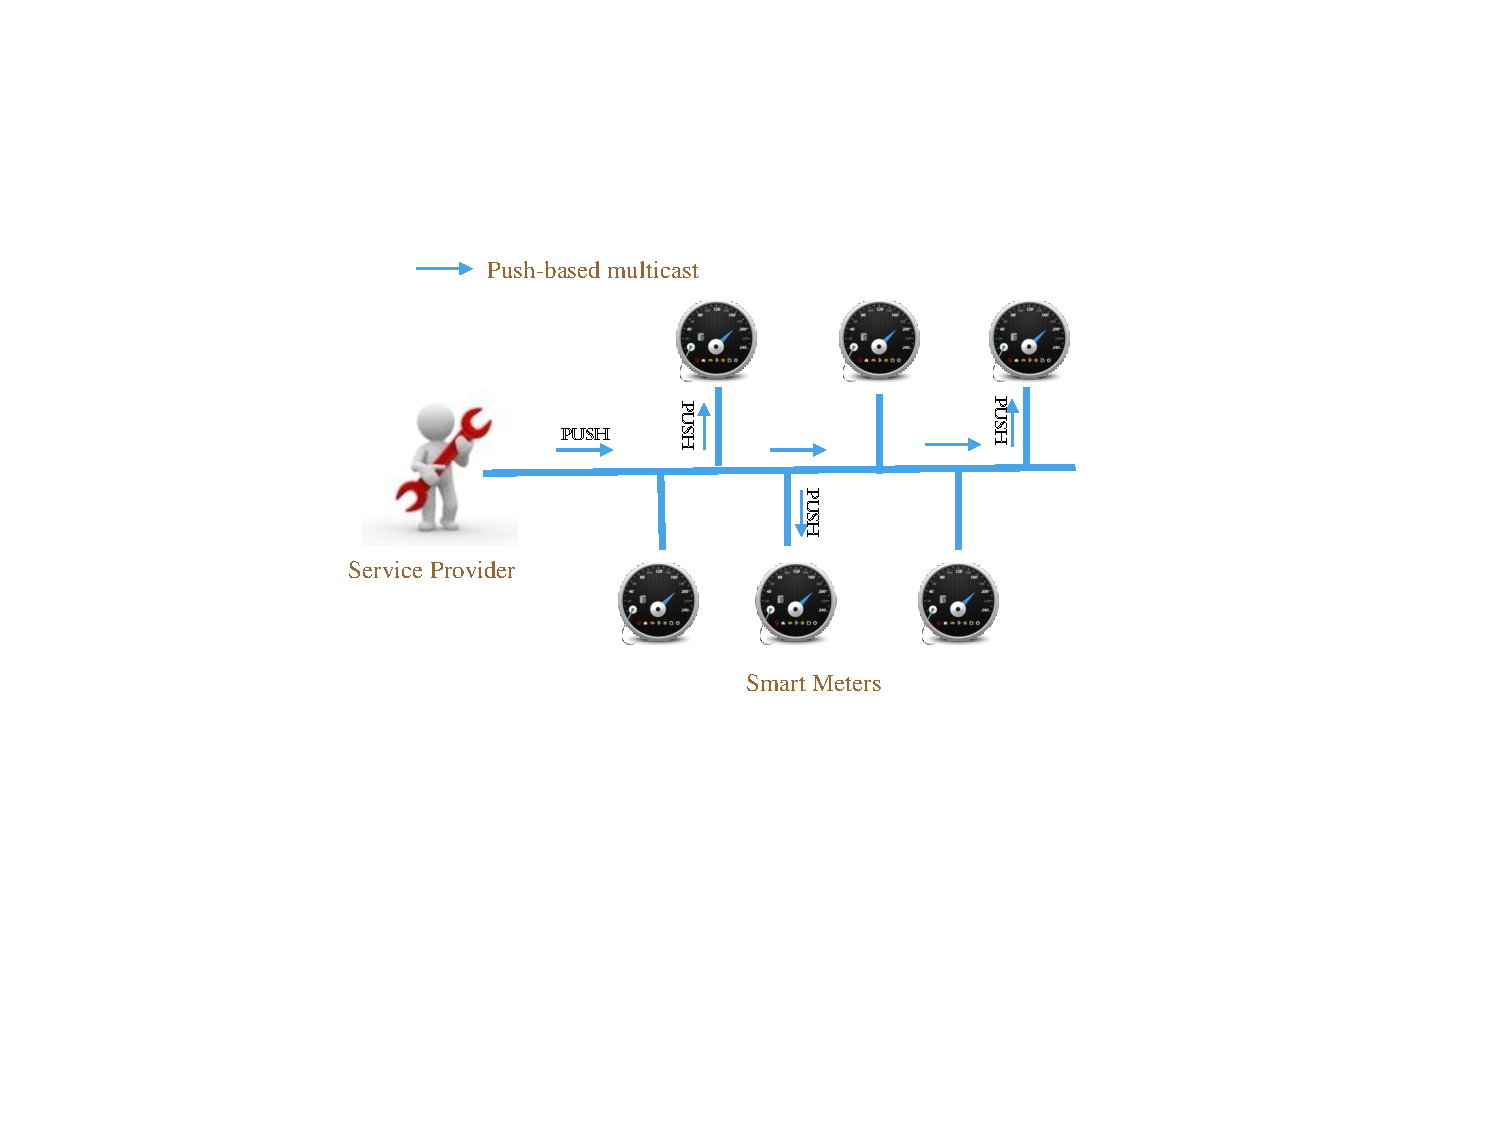
\includegraphics[width=8cm]{Smart_Grid_Architecture}\\
 \centering \caption{Commands broadcast  in smart metering}\label{sec:Fig1:Smart_Grid_Architecture}
\end{figure}

\begin{figure}[!htp]
\centering
 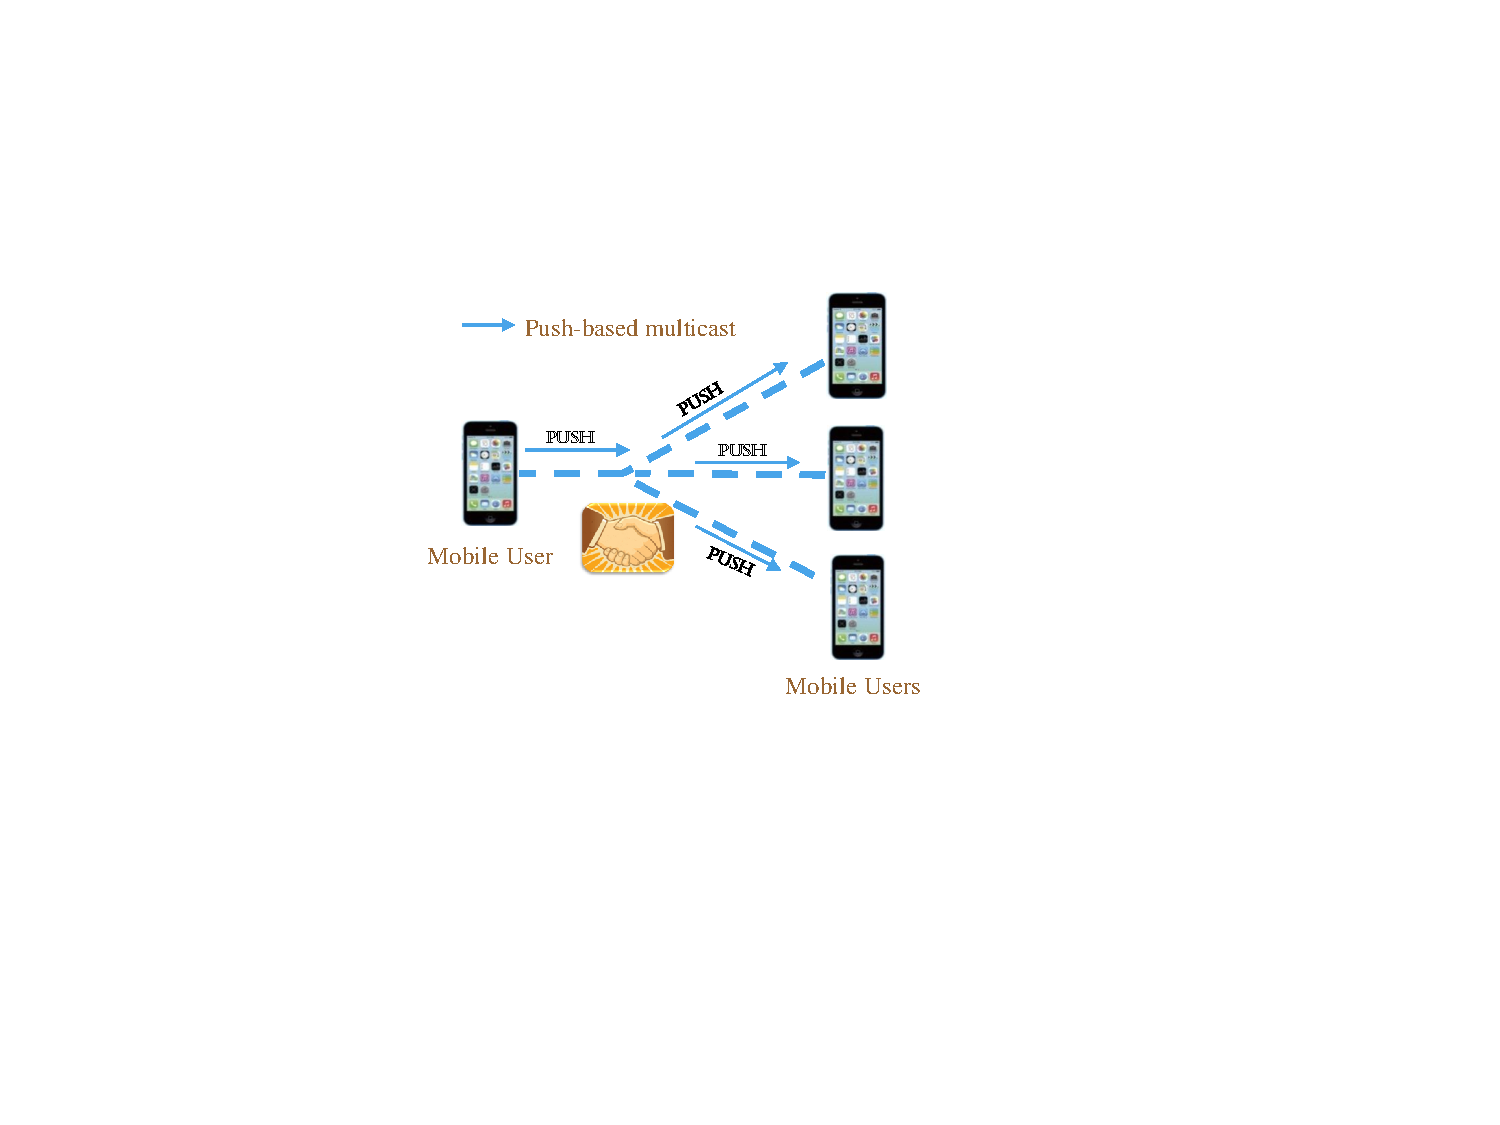
\includegraphics[width=8cm]{Social_network}\\
 \centering \caption{Friend discovery in Social networks}\label{sec:Fig2:Social_network}
\end{figure}




\subsubsection{Pull-based Multicast Communication}\label{sec:pull}
 A \emph{pull-based} secure multicast mechanism in which the data is stored after being generated and later is pulled by multiple authorized users may be as desirable for some cases in applications such as smart grids and body area networks. For example, multiple service providers may need to retrieve the electricity usage data of a smart meter for different purposes at different times; thus the smart meter should store its data at a data repository for future downloads. This poses significant security and privacy concerns because the access of the data in a data repository is completely out of the control of the smart meter who generated the data but it should be the smart meter's decision whether or not to disclose its electricity usage of certain smart devices to certain service providers -- a service provider in California may not need the utility usage data of a microwave in a house at Washington DC. Moreover, not all service providers need the same data. Thus smart meters should have the right to decide who should have the access right to their data. Fig.\ref{sec:Fig1:Smart_Grid_pull} illustrates such a pull-based multicast communication scenario in smart metering. Fig. \ref{sec:Fig2:BAN_pull} demonstrates a similar example in body area networks (BANs), in which the data collected by the body sensors is stored in a data repository and later accessed by different people for different purposes: the primary doctor has the full access rights to pull the patient's medical information while a nurse is able to read only the meta data.

 These applications require the data source to specify the set of users that can access the data: different users should have different access right to different data stored in the repository. Similar to the push-based multicast mentioned in Section~\ref{sec:push}, we resort to an access structure defined by the data source: only the user who possesses certain attributes can access the data stored in the data repository. This implies that the data source should store the access structure defining the access right in the repository as well.  Note that pull-based multicast allows the destinations to actively and asynchronously pull the data from the repository while push-based multicast feeds the data to all destinations at one time.

\begin{figure}[!htp]
\centering
 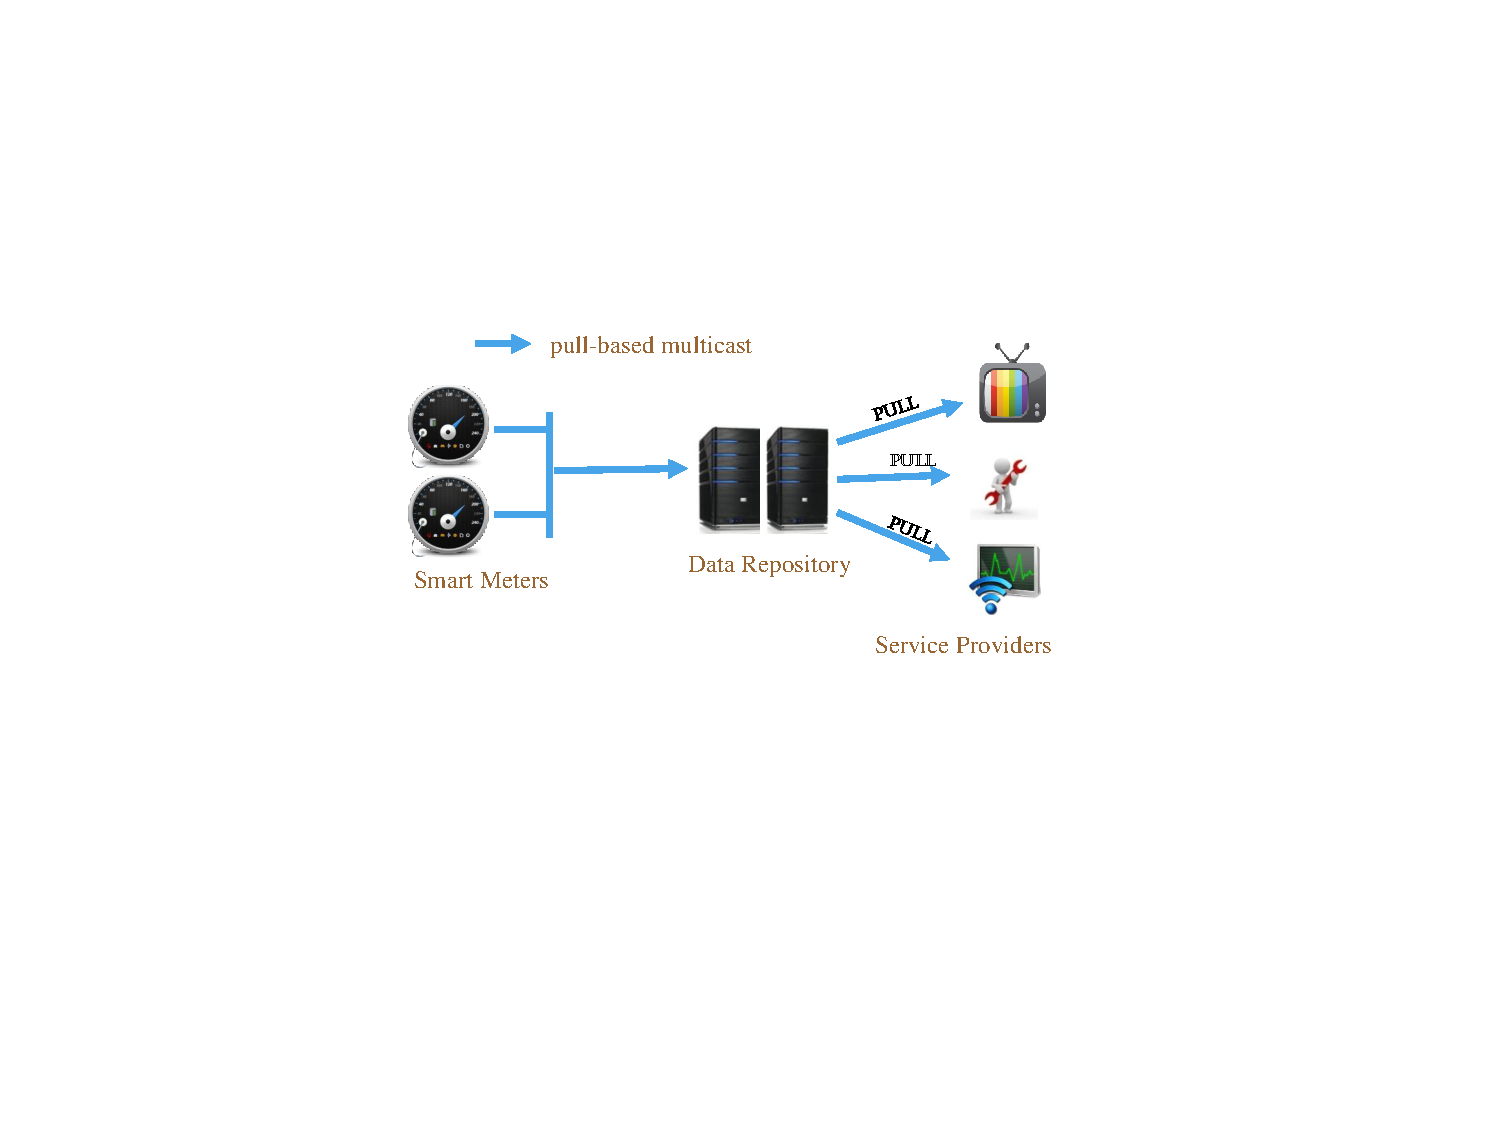
\includegraphics[width=8cm]{Smart_grid_pull}\\
 \centering \caption{Pull-based Multicast Communication in Smart Grid}\label{sec:Fig1:Smart_Grid_pull}
\end{figure}

\begin{figure}[!htp]
\centering
 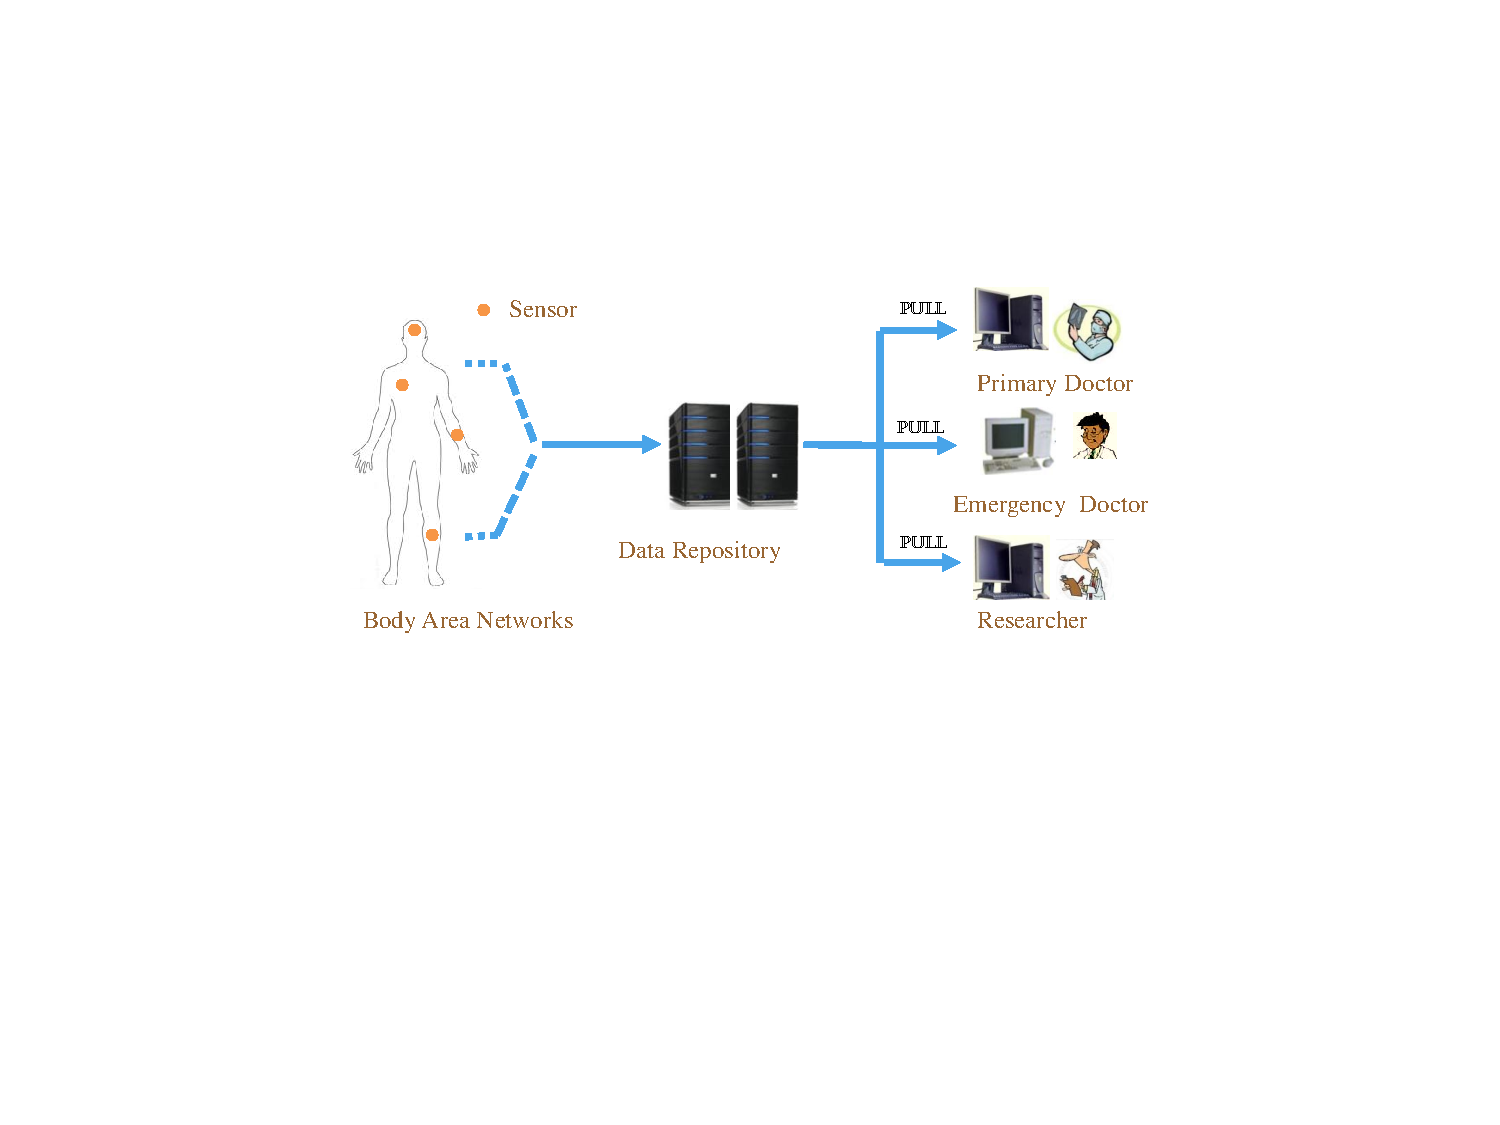
\includegraphics[width=8cm]{Body_Area_Networks_pull}\\
 \centering \caption{Pull-based Multicast Communication in BANs}\label{sec:Fig2:BAN_pull}
\end{figure}

%\begin{figure*}[t]\centering
%\begin{minipage}[t]{0.4\linewidth}
%\centering
%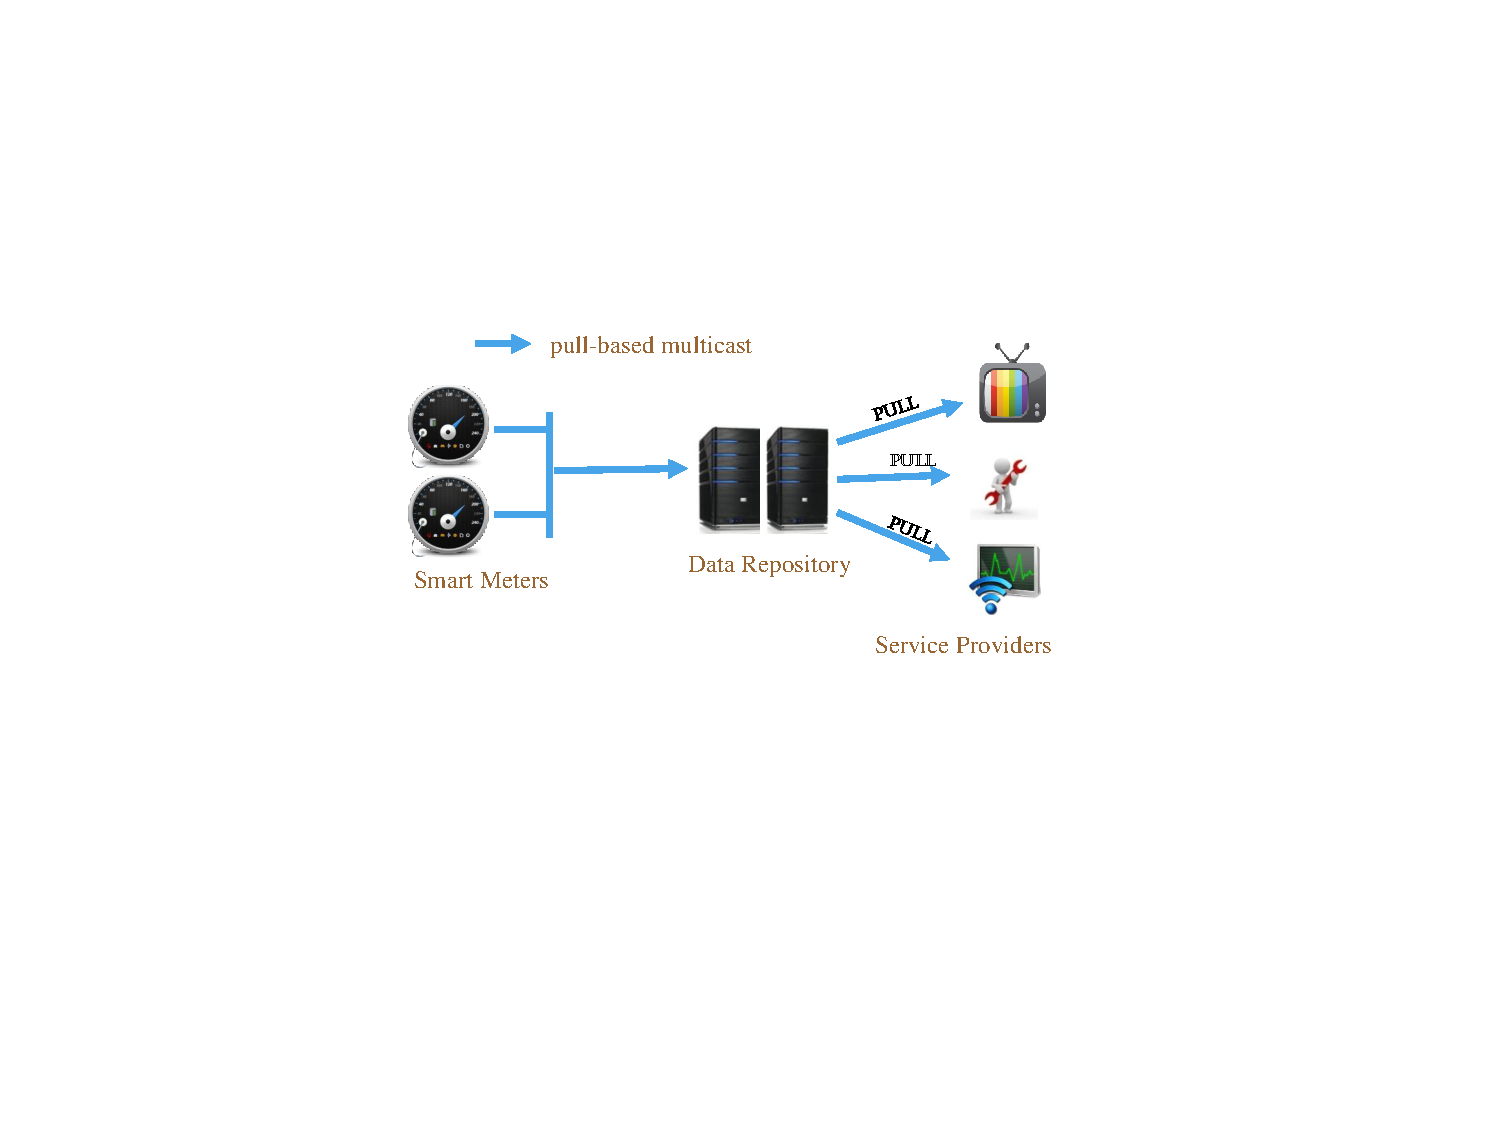
\includegraphics[height=28mm]{Smart_grid_pull}
%\caption{Pull-based Multicast Communication in Smart Grid} \label{sec:Fig1:Smart_Grid_pull}
%\end{minipage}
%\hspace {10mm}
%\begin{minipage}[t]{0.5\linewidth}
%\centering
%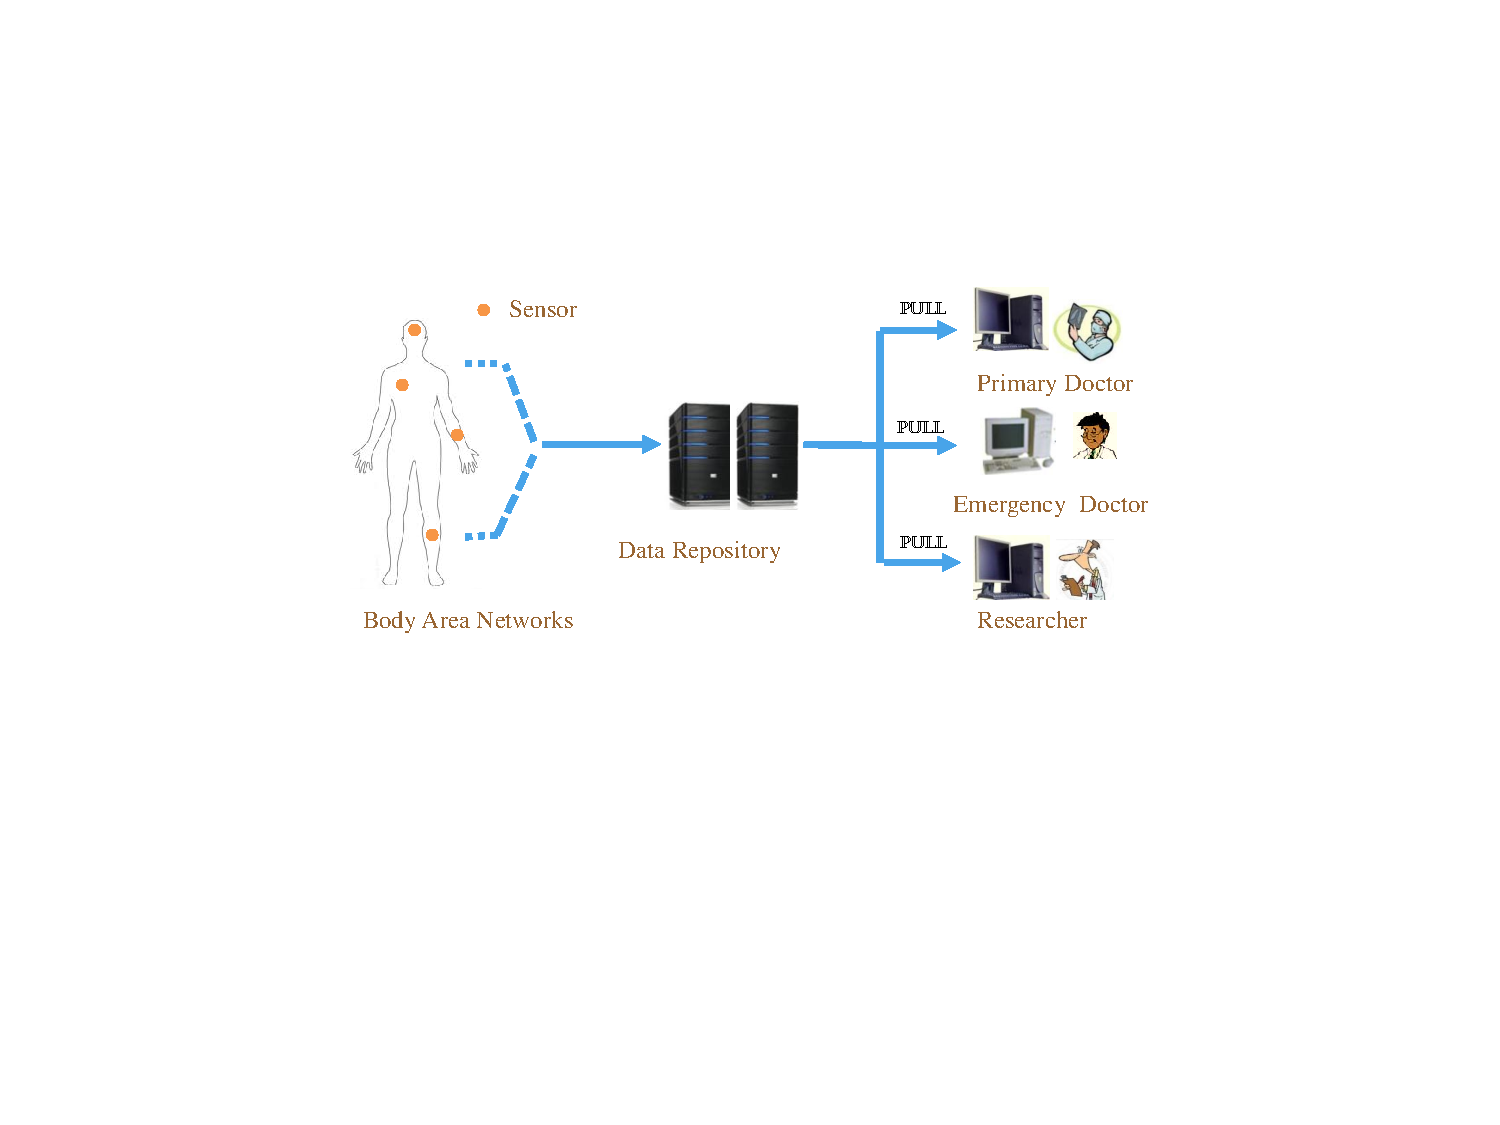
\includegraphics[height=28mm]{Body_Area_Networks_pull}
%\caption{Pull-based Multicast Communication in BANs} \label{sec:Fig2:BAN_pull}
%\end{minipage}
%\end{figure*}



\subsubsection{System Model}\label{sec:model}

We make the following observations from the application scenarios described in Sections~\ref{sec:push} and~\ref{sec:pull}: The multicast destinations are defined by a set of attributes forming an access structure specified by AND and OR relations. The message caring the data does not carry the identity of the destinations but carry an access structure: any user receiving the data is able to access the data only if it possesses the attributes specified in the access structure. Such multicast should provide access control, data encryption, confidentiality, and authentication to protect the data and the data source. These observations motivate us to consider a communication system depicted in Figure~\ref{Fig1:architecture}.

There are four entities in our system model: Key Generation Center (KGC), Data Source, Destinations, and Data Repository. The KGC generates and distributes keys for all entities. A data source produces the data to be broadcasted and defines the access structure of the data; it is assumed to have sufficient computational capacity to signcrypt the data. Destinations are defined by an access structure carried by the data; they are able to designcrypt a message and verify the authenticity of the source and the integrity of the data. A data repository stores signcrypted data generated by a data source.

\begin{figure}[!htp]
\centering
 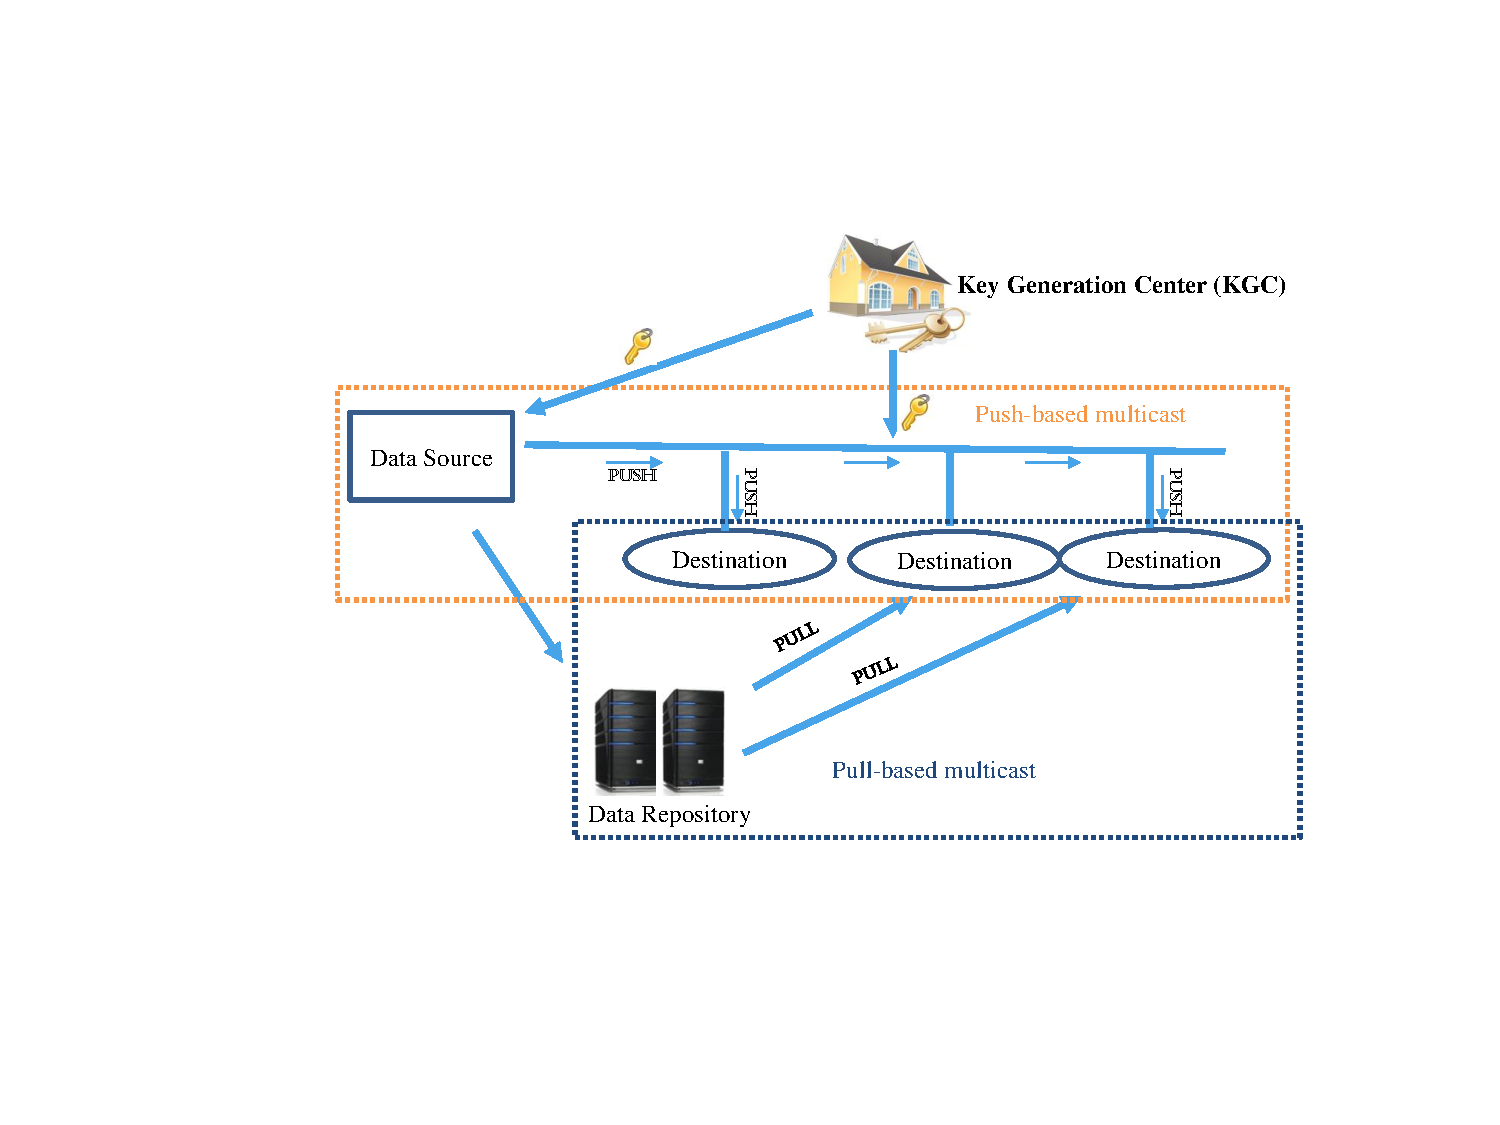
\includegraphics[width=10cm]{framework}\\
 \centering \caption{A generical communication architecture.}\label{Fig1:architecture}
\end{figure}

This system model involves two types of multicast communications: the multicast from a data source to all the destinations defined by an access structure (push-based multicast), and the retrieval of the data from a repository by multiple destinations (pull-based multicast).  The keys computed by KGC ensure that the data source's data is securely stored in a repository and retrieved only by authorized users when needed, and that the data is indeed generated by the data source and is not modified after being produced.

\subsubsection {Related works}
The most related works are IBE and ABE, which have received a significant amount of attention in recent years. There exists two different and complementary notions of ABE: Key-Policy ABE (KP\_ABE) \cite{goyal2006attribute} and Ciphertext-Policy ABE (CP\_ABE) \cite{bethencourt2007ciphertext}. In KP\_ABE, encryption is completely determined by the full set of descriptive attributes possessed by the data source while the decryption key is computed by a Key Generation Center (KGC) from an access policy defined by the KGC. In order to decrypt a ciphertext, a user must go to KGC to get a decryption key. In CP\_ABE, encryption is completely determined by an access tree defined from the set of attributes possessed by the data source, and the ciphertext carries the access policy; the decryption key is computed by KGC and is associated with a user possessing a certain set of descriptive attributes. In other words, KGC helps a user compute a deception key based on the user's attributes. A user can decrypt a ciphertext if and only if its attributes satisfy the access tree carried by the ciphertext.  Therefore in CP\_ABE, a data source is able to intelligently decide who should or should not have access to its data.  A new construction of CP\_ABE, named Constant-sized CP\_ABE (denoted as CCP\_ABE), was presented in \cite{zhou2010efficient}, which reduces the ciphertext length to a constant size for an AND gate access policy with any given number of attributes at the cost of long secret keys and complicated access structures.
%
A scheme that employs IBE to provide a zero-configuration encryption and authentication solution for end-to-end secure communications was proposed in \cite{so2010zero}. The concept of IBE was utilized by \cite{lu2012eppa} to construct a signature and later verify the signature. KP\_ABE was adopted by \cite{fadlullahtowards} to broadcast a single encrypted message to a specific group of users. The Lewko-Waters ABE scheme \cite{lewko2011decentralizing}, which was based on Linear Secret Sharing to construct the access policy, was used by \cite{ruj2011security}  to ensure access control. In this scheme, the remote terminal units (RTUs) are responsible for defining the access structure and uploading the encrypted data to the data storage center, which means that a data source has less control over its data. In our applications, messages can be modified, or dropped during transmissions. The receivers should verify the identity of the sender to protect against masquerading and spoofing. The above schemes can not ensure message integrity and confidentiality. A signcryption scheme based on KP\_ABE was proposed in \cite{gagne2010threshold}, which does not meet the requirements of many practical applications as the data source can not intelligently decide who should or should not have access to its data.
%
In this work, we present a signcryption scheme termed Ciphertext-Policy Attribute-Based SignCryption (CP\_ABSC) to provide the security services required by the multicast communications mentioned above. CP\_ABSC is applied to secure the push-based multicast as well as pull-based multicast. Compared to CP\_ABE, CP\_ABSC provides both encryption and signature without significantly increasing the computational cost (actually only the computational cost of designcryption is slightly increased compared to CP\_ABE due to signature verification in CP\_ABSC). CP\_ABSC has strong security strength in terms of collusion resistance, message authentication, forgery prevention, and confidentiality.

The contribution can be summarized as follows:
\begin{itemize}
\item We develop a novel scheme called Ciphertext-policy Attribute Based Signcryption (CP\_ABSC) based on CP\_ABE. The proposed scheme ensures security and privacy of the data by combining  signature and encryption without requiring a certificate for verification.
\item We prove the correctness of the proposed scheme and analyze its efficiency and feasibility. In particular,  we discuss  the security of the proposed scheme under four major attack scenarios: collusion, message authentication, forgery, and confidentiality. We also conduct a quantitative performance analysis, and our results indicate that the proposed CP\_ABSC is efficient and feasible.
\item We demonstrate how to apply the proposed signcryption scheme to secure different multicast communications in smart grids. Particularly, we develop a protocol to secure the instructions sent from utility companies to smart meters (push-based multicast); we also develop a procedure for the smart meter data to be securely stored and accessed by different  service providers based on CP\_ABSC (pull-based multicast). %\item We implement the scheme in an attribute based signature system and evaluate the performance in terms of computation cost.
\end{itemize}


\subsection{CP\_ABSC: A Ciphertext-Policy Attribute Based Signcryption Scheme}\label{sec:CP-ABSC}
%
%\subsubsection{Preliminaries}
%We now introduce the preliminary knowledge employed by the cryptographic algorithms of CP\_ABSC.
%
%\vspace{-3mm}



\subsubsection{Access Control Policy -- the Access Tree}
Our main idea is to design an attribute-based signcryption scheme that views an identity as a set of attributes, and
enforces a lower bound on the number of common attributes between a user's identity and its access rights specified by the sensitive
data. We use an access tree structure proposed by \cite{bethencourt2007ciphertext}, which is illustrated in Figure~\ref{Fig2:accesscontrol}, to control the user's access to the encrypted data. In Figure~\ref{Fig2:accesscontrol}, each non-leaf node $x$ is associated with two parameters, $num_x$ and $k_x$, where $num_x$ is the number of child nodes of node $x$, and $k_x\in[1,num_x]$ is its threshold value indicating that node $x$ performs the \emph{OR} operation over all subsets of $k_x$ child nodes of $x$, with each subset supporting an \emph{AND} operation; each leaf node $x$  is described by an attribute and a threshold value $k_x=1$. We also associate an index with each node $x$ in $T$, denoted by $index(x)$. Since a tree with $|S|$ number of attributes can have at most $2|S|-1$ nodes, we can assign a unique number in $\{1,2, \cdots, 2|S|-1\}$ to each node in the tree based on pre-order tree traversal. Other tree traversal techniques such as in-order or post-order can also be applied. Let $parent(x)$ be the parent node of $x$ in $T$.

\begin{figure*}[t]\centering
\begin{minipage}[t]{0.45\linewidth}
\centering
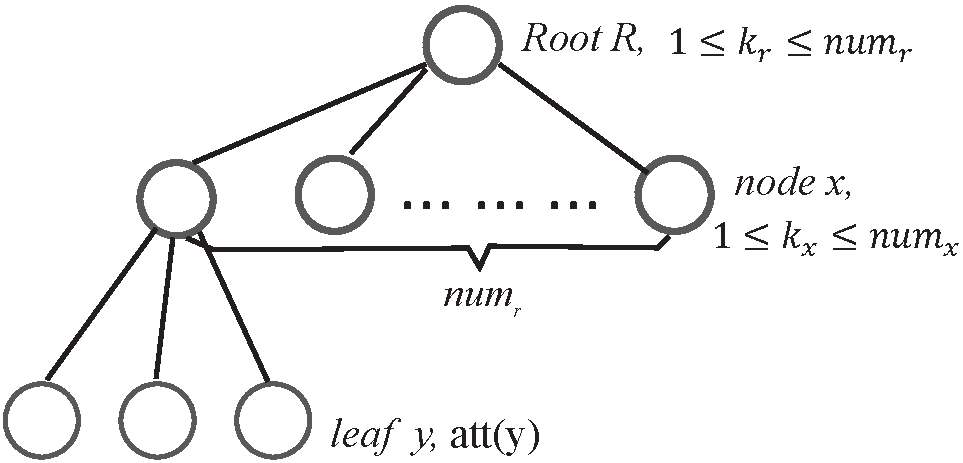
\includegraphics[height=30mm]{accesscontrol}
\caption{An access control tree structure} \label{Fig2:accesscontrol}
\end{minipage}
\hspace{6mm}
\begin{minipage}[t]{0.45\linewidth}
\centering
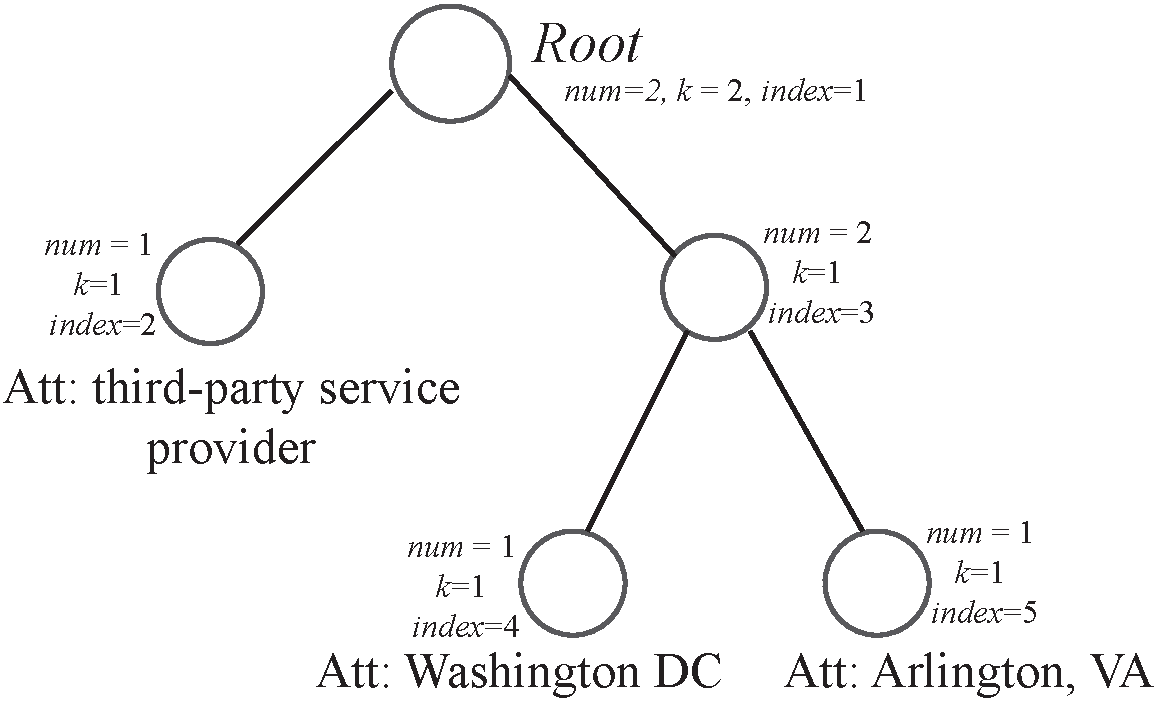
\includegraphics[height=30mm]{accesscontrolexample}
\caption{An example access control structure for a data item} \label{Fig2:accesscontrolexample}
\end{minipage}
\hspace{6mm}
\end{figure*}

%\begin{figure}[htp!]\centering
%  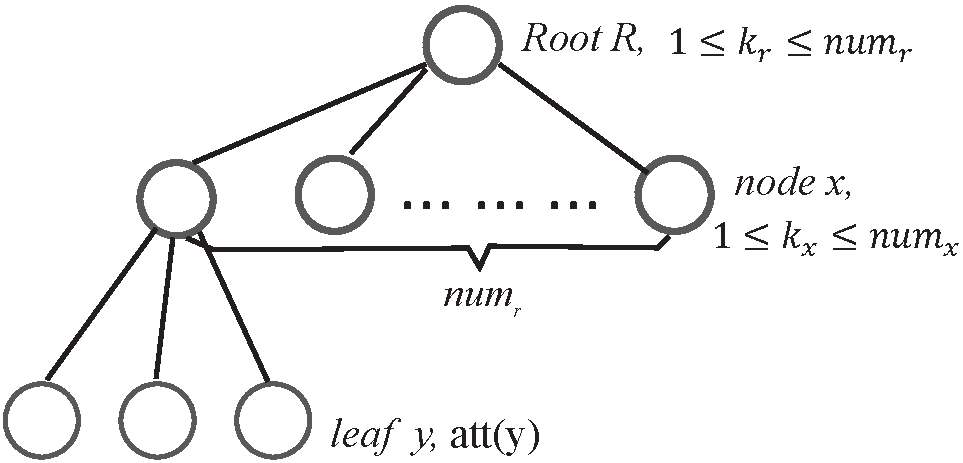
\includegraphics[width=7.5cm]{accesscontrol}\\
%  \caption{An access control tree structure.}\label{Fig2:accesscontrol}
%\end{figure}
%
Note that any attribute-based access structure can be represented by a tree $T$ shown in Figure~\ref{Fig2:accesscontrol}. For example,  the following access structure may be specified for a data item: (Third-Party Service Provider \emph{AND} (Arlington, VA \emph{OR} Washington, DC)), which indicates that only the third-party service providers in Arlington, VA or Washington, DC have the access to this data. Thus a user located in Washington DC with a set of attributes \{Third-Party Service Provider, Washington DC, Air-Conditioner\} has an access right to the data mentioned above.
The corresponding access control tree for this example is illustrated in Figure~\ref{Fig2:accesscontrolexample}. The indices of the root node and its two children are respectively 1, 2, and 3 based on pre-order tree traversal.
%
%\begin{figure}[h]\centering
%  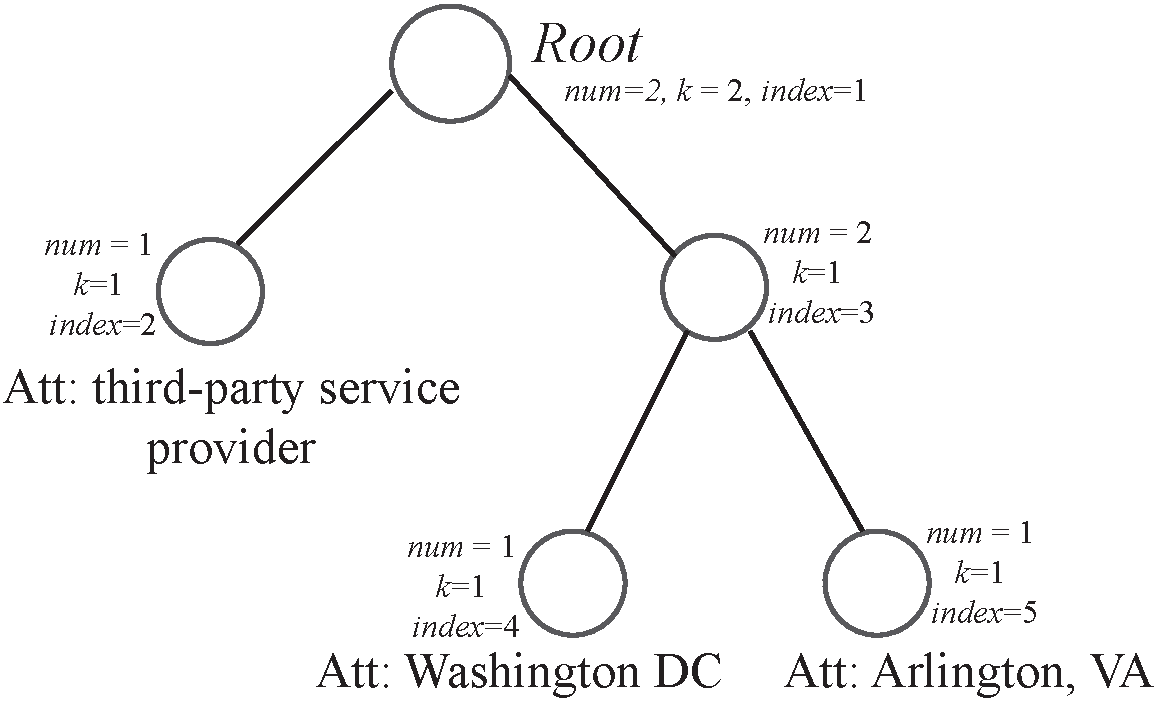
\includegraphics[width=7.5cm]{accesscontrolexample}\\
%  \caption{An example access control structure for a data item.}\label{Fig2:accesscontrolexample}
%\end{figure}
%
\subsubsection{CP\_ABSC: Ciphertext-Policy Attribute Based Signcryption}
In this subsection, we propose our CP\_ABSC, a Ciphertext-Policy Attribute-Based SignCryption scheme. CP\_ABSC consists of four primary algorithms. Algorithm \ref{alg:System initialization} is executed by KGC to provide system initialization. It generates and distributes to all the involved entities the public parameters of the system.

%system initialization
%=================================================
\begin{algorithm}[htp]
\caption{System Initialization}\label{alg:System initialization}
\begin{alginc}
\State Select a prime $p$, the generators $g_1$ and $g_2$  for $\mathbb{G}_1$ and $\mathbb{G}_2$, respectively,  and a bilinear mapping $e:  \mathbb{G}_1 \times \mathbb{G}_2 \rightarrow \mathbb{G}_3$.
\State Choose two random exponents $\alpha, \beta \in \mathbb{Z}_p$.
\State Select a hash function  $H_1: \{0,1\}^\ast \rightarrow\mathbb{Z}_p$.  This function $H_1$ is viewed as a random oracle.
\State Publish the public parameters given by
 \begin{equation}
PK=(p,\mathbb{G}_1,\mathbb{G}_2, H_1, g_1, g_2, h=g_1^\beta, t= e(g_1,g_2)^\alpha)
\end{equation}
\State Compute the master key $MSK=(\beta, g_2^\alpha)$.
\end {alginc}
\end{algorithm}

Algorithm \ref{alg:KeyGeneration} is also executed by \emph{KGC} to generate three keys for an attribute set $S$: the key $SK$ for ciphertext designcryption, the signing key $K_{sign}$ for signing the ciphertext message, and the verification key $K_{ver}$ for signature verification.
%Encryption is done according to the access tree defining the attribute-based access policy and thus no special encryption key is needed (see Algorithm~\ref{alg:Encryption}).
For example, a utility company possessing the attribute set $S$ can use its signing key $K_{sign}$ to sign its commands or instructions sent to the smart meters, and use its designcryption key $SK$ to designcrypt the smart meter data stored in ciphertext format (signcrypted data) at the data repositories; its verification key  $k_{ver}$ is published for others to verify the signature of its ciphertext.


\begin{algorithm}[htp]
\caption{Key Generation (\emph{MSK}, $S$)}\label{alg:KeyGeneration}
\small{\bf Inputs:} The master key \emph{MSK} and a set of attributes $S$ belonging to an entity.
\begin{alginc}
\State Select random numbers $r_{en},r_{sn} \in \mathbb{Z}_p$
\State Compute the secret key component $D_{en}=g_2^{\frac{(\alpha+r_{en})}{\beta}}$ and signing key $K_{sign}=g_2^{\frac{(\alpha+r_{sn})}{\beta}}$.
\For {each attribute $j\in S$}
  \State Select a random number $r_j \in \mathbb{Z}_p$
  \State Compute the secret key components $$D_j=g_2^{r_{en}}\cdot g_2^{(H_1(j)\cdot {r_j})} \mbox{ and } D_j^\prime=g_2^{r_j}$$
\EndFor
\State The secret key $SK$ for designcryption is:
\begin{equation}
 SK= (D_{en}, \forall j \in S: D_j, D_j^\prime).
\end{equation}
\State Compute the verification key:  $K_{ver} = g_2^{r_{sn}}$
\State Send $SK$ and $K_{sign}$ to the owner of the attribute set $S$, and  publish $K_{ver}$ for others to verify the owner of $S$.
\end{alginc}
\end{algorithm}

Algorithm \ref{alg:Encryption} details the signcryption procedure, which is the core of the proposed CP\_ABSC. This algorithm is mainly performed by data sources (a smart meter or a service provider) to signcrypt its data before transmitting to the data repositories or to other receivers (e.g., smarter meters are the receivers of an instruction).  In a typical application, a data source encrypts a message/data whose access control is specified by an access tree $T$, and signs the message with its signing key. Note that Lines 1 to 7 is executed only once for all the data with the same access structure. Algorithm \ref{alg:Encryption} is designed to provide confidentiality, access control, integrity, authentication, and non-repudiation to ensure the security and privacy of the data sources. Note that encryption is completely determined by the access policy of the data itself.

\begin{algorithm}[htp]
\caption{SignCryption\emph{(M, T, $K_{sign}$)}}\label{alg:Encryption}
\small{\bf Inputs:} The public parameter $PK$; plaintext message $M$; the tree $T$ rooted at node $R$ specifying the access control policy of message $M$; and the signing key $K_{sign}$.
\begin{alginc}
\State Choose a polynomial $q_x$ and sets its degree $d_x=k_x-1$ for each node $x$ in the tree $T$.
\State Choose a random number $s\in \mathbb{Z}_p$ and sets $q_R(0)=s$;
\State Choose $d_R$ random numbers from $\mathbb{Z}_p$ to completely define the polynomial $q_R$.
  \For {any other node $x$ in $T$}
  \State Set $q_x(0)=q_{parent(x)}(index (x))$.
  \State Select $d_x$ random numbers from $\mathbb{Z}_p$ to completely define $q_x$.
  \EndFor
\item Let $Y$ be the set of leaf nodes in $T$. The ciphertext $CT$ is constructed based on the access tree $T$ as follows:
\begin{eqnarray}
 CT&=& ( T, \tilde {C}=M\oplus t^{s}, C=h^s, \nonumber\\
 & & \forall y\in Y: C_y=g_1^{q_y(0)}, \nonumber\\
 & & \hspace{1.4cm} C_y^\prime=g_1^{(H_1(att(y))\cdot {q_y(0)})})
\end{eqnarray}
\State Choose a random $\zeta \in \mathbb{Z}_p$; compute $\delta=e(C,g_2)^\zeta$, $\pi=H_1(\delta|M)$, and $\psi=g_2^\zeta\cdot (K_{sign})^\pi$.
\State Output the message:
\begin{eqnarray}
 CT_{sign}&=& ( T, \tilde {C}, C, \forall y\in Y: C_y, C_y^\prime; W=g_1^s, \pi,\psi)\nonumber
\end{eqnarray}
\end{alginc}
\end{algorithm}


Algorithm \ref{alg:decryption} implements verification and decryption. The ciphertext receivers execute it to decrypt the ciphertext according to their attributes. Note that Algorithm \ref{alg:decryption}  calls a function \emph{DecryptNode} described in Algorithm \ref{alg:function}, which was originally proposed by \cite{bethencourt2007ciphertext}. Here we include \emph{DecryptNode} for completeness and to help the readers without the knowledge of CP\_ABE to understand CP\_ABSC.


%Decryption Algorithm
\begin{algorithm}[!htb]
\caption{DeSignCryption (\emph{$CT_{sign}$}, \emph{SK}, $S$)}\label{alg:decryption}
\small{{\bf Inputs:} The $CT_{sign}=(CT, W, \pi,\psi)$; the private key $SK$ for designcryption; and the set of possessed attributes $S$.
}
\begin{alginc}

\State $A=DecryptNode (CT, SK, R)$
 \If {$A\ne\perp$}
  \State $\tilde {A}= e(C,D_{en})/A$
 \EndIf
 \State Compute
 \begin{equation}
   \delta^\prime=\frac{e(C,\psi)}{(e(W,K_{ver})\cdot \tilde {A})^\pi}
 \end{equation}\label{equ:verification}
 \If {$H_1(\delta^\prime|M^\prime)=\pi$}
   \State return $M = M^\prime$
\EndIf
\State Return $\perp$

\end{alginc}
\end{algorithm}
%=================================================

\begin{algorithm}[!ht]
\caption{Function \emph{DecryptNode $(CT, SK, x)$}}\label{alg:function}
\small{{\bf Inputs:} A ciphertext $CT=( T, \tilde{C}, C, \forall y \in Y: C_y, C_y^\prime)$; the secret key $SK$, which is associated with a set $S$ of attributes, the node $x$ from $T$.
}
\begin{alginc}
    \If {$x$ is a leaf node of $T$}
    \State Let $i= att (x)$
     \If {$i \in S$}
       \begin{eqnarray}
       \mbox{Return } F_x=\frac {e(C_i, D_i)}{e(C_i^\prime, D_i^\prime)}=e(g_1,g_2)^{r_{en}q_x(0)}
      \end{eqnarray}
        \Else  \;\;Return $\perp$
        \EndIf
        \Else
        \For {Each child node $z$ of $x$}
            \State $F_z = DecryptNode (CT,SK,z)$
        \EndFor
        \EndIf
       \State Let $S_x$ be an arbitrary $k_x$-sized set of child nodes of $x$ such that $F_z\ne\perp$ for $\forall z\in S_x$.
        \If {$S_x$ exists}
        \For {Each node $z\in S_x$}
        \State $i_z =index(z)$
        \State $S_z^\prime=\{index(z)\;||\; z\in S_x\}$
        \State $\triangle_{i_z,S_z^\prime}(y)=\prod_{j\in S_z^\prime,j\neq i_z}\frac{y-j}{i_z-j}$
        \EndFor
       \State Return \begin{eqnarray*}
 F_x&=& \prod_{z\in S_x} F_z^{\triangle_{i_z,S_z^\prime}(0)}\\
 &=&\prod_{z\in S_x}(e(g_1,g_2)^{r_{en}\cdot q_z(0)})^{\triangle_{i_z,S_z^\prime}(0)}\\
 &=& \prod_{z\in S_x} e(g_1,g_2)^{r_{en} \cdot q_x(i_z) \cdot {\triangle_{i_z,S_z^\prime} (0)}}\\
 &=& e(g_1,g_2)^{r_{en} \cdot q_x(0)}
\end{eqnarray*}.
%\State Return $F_x$
        \Else
        \State Return $F_x=\perp$
        \EndIf
\end{alginc}
\end{algorithm}


\subsubsection{CP\_ABSC v.s. CP\_ABE}

In this section, we compare CP\_ABSC and CP\_ABE\cite{bethencourt2007ciphertext} to illustrate their differences. The characteristics of CP\_ABSC and CP\_ABE are summarized in Table \ref{table:comparison between CP-ABE and our scheme}.

%\begin{table*}[tb]
%\caption{Comparison  between CP\_ABE and CP\_ABSC}\label{table:comparison between CP-ABE and our scheme}
%\centering
%\begin{tabular}{c| c| c|c|c}
%\hline
%The scheme& System Initialization & Key Generation & Encryption  & Decryption\\
%\hline
%CP\_ABE~\cite{bethencourt2007ciphertext} & symmetric groups & private key & encryption & decryption \\
%CP\_ABSC & asymmetric groups & (private+signature) key & signcryption & decryption\& verification\\
%\hline
%\end{tabular}
%\end{table*}


\begin{table*}[tb]
\caption{Comparison  between CP\_ABE and CP\_ABSC}\label{table:comparison between CP-ABE and our scheme}
\centering
\begin{tabular}{c| c| c}
\hline
The scheme&  CP\_ABE~\cite{bethencourt2007ciphertext} & CP\_ABSC  \\
\hline
System Initialization & symmetric groups & asymmetric groups \\
Key Generation & private key  & (private+signature) key \\
Encryption & encryption& signcryption\\
Decryption & decryption& decryption\& verification\\
\hline
\end{tabular}
\end{table*}

\emph{ System Initialization}: The system initialization procedure creates the groups, the group generators, and the bilinear mapping. The difference between CP\_ABSC and CP\_ABE is that the former uses asymmetric groups while the latter uses symmetric groups.

\emph{Key Generation}: The Key Generation algorithm in our scheme CP\_ABSC is different from the key generation in CP\_ABE \cite{bethencourt2007ciphertext} in two aspects: i) since we are designing a signcryption scheme, we need to compute a signing key (which will be sent to the signcryptor) and a verification key (which will be public) while CP\_ABE only needs one key for decryption; and ii ) due to the fact that CP\_ABSC utilizes asymmetric groups, its key generation is more computationally efficient than the one proposed in \cite{bethencourt2007ciphertext} according to our comparison study in Section \ref{sec:performance analysis}.

\emph{ Encryption (SignCryption)}: The SignCryption algorithm in our scheme CP\_ABSC combines signature and encryption, while the one in \cite{bethencourt2007ciphertext}  performs only encryption. The computational cost of our SignCryption algorithm is less than the sum of the two computations (encryption and signature), and is also less than that of the encryption algorithm in \cite{bethencourt2007ciphertext}, according to our analysis in Section \ref{sec:performance analysis}, which is attributed to the adopted asymmetric groups.

  \subsubsection {Decryption (DeSignCryption)} The DeSignCryption in CP\_ABSC includes decryption and verification, while the decrypt algorithm in \cite{bethencourt2007ciphertext} performs only decryption. The computational cost of DeSignCryption is only slightly higher than that of the decyption algorithm in \cite{bethencourt2007ciphertext}, according to our analysis in Section \ref{sec:performance analysis}.

Note that our scheme has a performance boost compared to CP\_ABE. In practice, it's more straightforward to do signcryption in just one operation.

\subsubsection{Application of CP\_ABSC in Smart Grids}\label{sec:application}

In this section, we illustrate how to use CP\_ABSC to secure the two typical multicast communications in a smart grid.  %in Figure~\ref{Fig1:architecture}.

Initially, the KGC computes the public parameters $PK$ according to Algorithm~\ref{alg:System initialization}, and posts $PK$ to all active entities (smart meters and service providers) in the system. Each active entity also needs to register with the KGC to get the corresponding keys computed from Algorithm \ref{alg:KeyGeneration}. For example, a utility company needs a private key $SK$ for designcryption based on its access attributes, a signing key $K_{sign}$ to sign its commands, and a verification key $K_{ver}$ for others to verify the signature of its ciphertext. %Meanwhile, the KGC publishes the corresponding verification key $K_{ver}$.

\emph{Push-based multicast communication in smart grid}

When a service provider wants to send instructions or commands to one or more smart meters, the service provider constructs an access structure $T$ that describes the set of smart meters satisfying the access policy. It then signcrypts an instruction $I$ with a timestamp $ts$. The timestamp can be the current time or the current time with an expiration time. Generally speaking, the timestamp can help the receivers decide whether or not instruction $I$ is valid and resist replay attacks.   The following procedure implements a push-based multicast for a service provider to broadcast $I$ to certain smart meters.
%
\begin{enumerate}
\item The service provider signcrypts $I||ts$ with Algorithm~\ref{alg:Encryption}, and then broadcasts an encrypted instruction to the smart meters:
\begin{equation}
\begin{split}
Service\;  provider\rightarrow Smart\; meters:\\
 SignCryption(I||ts, T, K_{sign}).\nonumber
\end{split}
\end{equation}

\item When a smart meter obtains the signcrypted instruction $SignCryption(I||ts, T, K_{sign})$, it designcrypts and verifies the message according to Algorithm~\ref{alg:decryption}. If the verification is passed, the smart meter executes the instruction and sends a response to the service provider to notify that it has received the instruction (proving that it has the required privilege).
%\begin{equation*}
%\begin{split}
% Smart\; meter \rightarrow Service \; provider: h^\prime=H_1(I||ts).
%\end{split}
%\end{equation*}

\item  When the service provider receives the feedback response, the communication is completed; otherwise, the service provider sends the instruction again.
\end{enumerate}

\emph{Pull-based multicast communication in smart grid} \label{sec:sec:data communication}

In order to protect the power usage data, a smart meter signcrypts the data of its household devices using Algorithm \ref{alg:Encryption}  based on the access policy specified by the data, and then sends the signcrypted data $CT_{sign}$ to a data repository. When  a service provider  possessing an attribute set $S$ wants to get the data for a particular household device, it contacts the data repository and gets the signcrypted data $CT_{sign}$. The following procedure details the process implementing a pull-based multicast.
%
\begin{enumerate}
\item A smart meter signcrypts its reading $M$ with a timestamp $ts$, $M||ts$, based on Algorithm~\ref{alg:Encryption} and then sends $CT_{sign}$ to the data repository. This step can be performed whenever a new data item is generated.
\begin{equation}
\begin{split}
Smart\;  meter\rightarrow Data\; repository:
CT_{sign}.\nonumber
\end{split}
\end{equation}

\item When a service provider holding an attribute set $S$ needs to access the smart meter data, it contacts the data repository to obtain the signcrypted data $CT_{sign}$:
\begin{equation*}
\begin{split}
Data\; repository \rightarrow Service\; provider: CT_{sign}.\nonumber
\end{split}
\end{equation*}

\item Upon receiving the signcrypted data $CT_{sign}$, the service provider designcrypts $CT_{sign}$ and verifies the message according to Algorithm~\ref{alg:decryption}: it first recovers the plaintext $M^\prime$ based on its private key $SK$ and then computes $\delta^\prime$; if  $H_1(\delta^\prime|M^\prime) = \pi$, which demonstrates the successful designcryption of the data, the service provider accepts $M^\prime$; otherwise, the message is dropped.

\end{enumerate}

\subsection{Correctness and Performance Analysis}\label{sec:correctness_performance}

In this section, we prove the correctness of CP\_ABSC and analyze its security strength. We also carry out a simulation based performance analysis to quantitatively study the efficiency and computational cost of CP\_ABSC.

\subsubsection{The Correctness of CP\_ABSC}
In this subsection, we show that CP\_ABSC is indeed feasible and correct. We claim that
Algorithm \ref {alg:decryption} can correctly decrypt the ciphertext if the designcryptor satisfies the access policy, and can verify whether the received message has been forged or falsified, and whether the received message is indeed sent by the message owner.

First, from the decryption procedure we have
\begin{eqnarray*}
 M^\prime&= &\tilde{C}\oplus \tilde{A}\\
 & = & \tilde{C}\oplus(\frac{e(C,D)}{A}) \\
  &=&\tilde{C}\oplus(\frac{e(C,D)}{A})\\
 & = & \tilde{C}\oplus(\frac{e(h^s, g_2^{(\alpha+r_{en})/\beta})}{e(g_1,g_2)^{r_{en}s}})\\
 &=& M\oplus e(g_1,g_2)^{\alpha s}\oplus(\frac{e(g_1^{\beta s},g_2^{\alpha+r_{en}/\beta})}{e(g_1,g_2)^{r_{en}s}})\\
 &=& M\oplus e(g_1,g_2)^{\alpha s}\oplus(\frac{e(g_1,g_2)^{\beta s \cdot (\alpha+r_{en})/\beta}}{e(g_1,g_2)^{r_{en}s}})\\
 &=& M\oplus e(g_1,g_2)^{\alpha s}\oplus(\frac{e(g_1,g_2)^{(\alpha s+r_{en}s)}}{e(g_1,g_2)^{r_{en}s}})\\
 &=& M\oplus e(g_1,g_2)^{\alpha s}\oplus e(g_1,g_2)^{\alpha s} \\
 &=& M.
\end{eqnarray*}
which indicates that Algorithm \ref{alg:decryption} can correctly decrypt the ciphertext if the designcryptor satisfies the access policy (posessing the designcryption key $SK$).

Second, the receiver verifies whether the message $M^\prime$ has been forged or falsified, and whether the received message is indeed sent by the generator of the message. The designcryptor (the receiver) computes $\delta^\prime$ by:
\begin{eqnarray*}
 \delta^\prime&=&\frac{e(C,\psi)}{(e(W,K_{ver})\cdot \tilde {A})^\pi}\\
 &=&\frac{e(g_1^{{\beta}s},g_2^{\zeta}\times g_2^{\frac{(\alpha+r_{sn})}{\beta}\pi})}{(e(g_1^s,g_2^{r_{sn}})\cdot e(g_1,g_2)^{{\alpha}s})^\pi}\\
 &=&e(g_1,g_2)^{\beta s (\zeta + {\frac{(\alpha+r_{sn})}{\beta}\pi}) - s r_{sn} \pi - \alpha s \pi}\\
 &=&e(g_1,g_2)^{\beta s \zeta + s (\alpha+r_{sn}) \pi - s r_{sn} \pi - \alpha s \pi}\\
 &=&e(g_1,g_2)^{\beta s \zeta}=e(C,g_2)^\zeta  \\
 &=& \delta.
\end{eqnarray*}
%
If $H_1(\delta^\prime|M^\prime) = \pi$,  $M^\prime$ is valid, i.e., $M = M^\prime$, and the message is not modified and is indeed sent by the generator; otherwise, $M^\prime$ is invalid.



\subsubsection{Security Strength}\label{subsec:security analysis}
In this subsection, we analyze the security strength of the proposed scheme CP\_ABSC by examining how it can counter four major attacks.

\emph{Collusion}\label{subsubsec:collusion attacks}
In CP\_ABSC, the set of attributes composes of the user's identity. In order to provide different types of users with different access rights, the scheme provides an access tree structure for each signcrypted data item, and requires only  a subset of the attributes for designcryption.  Since the secret key computation involves a unique random number for each attribute in the access policy, our scheme can defend against collusion attacks.

For example, assume that neither user $U_1$ nor user $U_2$ possesses a sufficient number of attributes to successfully designcrypt the ciphertext $CT_{sign}$ alone but the combined attribute set has sufficient number of attributes for the designcryption.  Then $U_1$ and $U_2$ may collude by combining their attributes. However, they are not able to combine their secret keys (the $SK$s) to get a secret key for the combined set of attributes according to Algorithm \ref{alg:KeyGeneration} because the KGC generates different random numbers $r_{en}$ for $U_1$ and $U_2$.
Thus they could not designcrypt the message, and the proposed scheme is secure against collusion attacks.

\emph{Message Authentication}: Assume that a user $U$ wants to get a message $M$ from the data repository. Before the data is stored in the data repository, the data generator has signcrypted it with  Algorithm \ref{alg:Encryption}. When $U$ plans to obtain the data from the data repository, it needs its private key $SK= (D=g_2^{\frac{(\alpha+r_{en})}{\beta}}, \forall j \in S: D_j=g_2^{r_{en}}\cdot g_2^{(H_1(j)\cdot {r_j})}, D_j^\prime=g_2^{r_j})$, which is computed by  Algorithm~\ref{alg:KeyGeneration}. Meanwhile, $U$ obtains the data source's verification key from KGC. It designcrypts the ciphertext to get the message $M^\prime$ by  Algorithm \ref{alg:decryption}: if $H_1(\delta^\prime|M^\prime) = \pi$ is established, the decrypted message \emph{M} is valid; otherwise, it is discarded.

%\begin{table*}[tb]
%\caption{The details of Functions and Operations between CP\_ABE and our scheme}\label{table:comparison computation cost between CP-ABE and our scheme}
%\centering
%\begin{tabular}{l| p{4cm}| p{5cm}| p{3cm}}
%\hline
%The scheme& Key Generation & Encryption & Decryption \\
%\hline
%CP\_ABE~\cite{bethencourt2007ciphertext} & $n\Gone + (n+2)\Gtwo + nH_{\Gtwo}$ & $(k+1)\Gone + k\Gtwo + 1\Gthree + kH_{\Gtwo}$& $(2k^\prime + 1)$ (pairings) \\
%CP\_ABSC & $(2n+5)\Gtwo$ & $(2k+2)\Gone + 2\Gtwo + 2\Gthree + 2$ (pairings) & $(2k^\prime+3)$ (pairings) \\
%\hline
%\multicolumn{4}{p{13cm}}{Notes: $\Gone$ in the table means an exponentiation operation in $\Gone$ group; $\Gtwo$ and $\Gthree$ are defined similarly. $H_{\Gone}$ means hashing an attribute string or a message into an element in $\Gone$; $H_{\Gtwo}$ is defined similarly.}
%\end{tabular}
%\end{table*}


\begin{table*}[tb]
\caption{The details of Functions and Operations between CP\_ABE and our scheme}\label{table:comparison computation cost between CP-ABE and our scheme}
\centering
\begin{tabular}{l| c| c}
\hline
   & CP\_ABE~\cite{bethencourt2007ciphertext}  & CP\_ABSC  \\
\hline
Key Generation&$n\Gone + (n+2)\Gtwo + nH_{\Gtwo}$ & $(2n+5)\Gtwo$\\
Encryption&$(k+1)\Gone + k\Gtwo + 1\Gthree + kH_{\Gtwo}$&$(2k+2)\Gone + 2\Gtwo + 2\Gthree + 2$ (pairings) \\
Decryption&$(2k^\prime + 1)$ (pairings)&$(2k^\prime+3)$ (pairings)\\
\hline
\multicolumn{3}{p{12cm}}{Notes: $\Gone$ in the table means an exponentiation operation in $\Gone$ group; $\Gtwo$ and $\Gthree$ are defined similarly. $H_{\Gone}$ means hashing an attribute string or a message into an element in $\Gone$; $H_{\Gtwo}$ is defined similarly.}
\end{tabular}
\end{table*}

\begin{table*}[tb]
\caption{The Computational Cost (Run Time) of Different Operations in Charm Library}\label{table:charmBenchmark}
\centering
\begin{tabular}{c|c|c|c|c|c|c}
\hline
Group & $\Gone$ & $\Gtwo$ & $\Gthree$ & (pairings) & $H_{\Gone}$ & $H_{\Gtwo}$ \\
\hline
SS512 &  3.73 & 3.70 & 0.48 & 3.92 & 8.34 & 8.39\\
MNT159 & 1.12 & 9.84 & 2.62 & 8.42 & 0.10 & 34.82\\
\hline
\multicolumn{7}{p{8cm}}{Notes: Time is in ms. The result in this table is the average of 1000 runs.}
\end{tabular}
\end{table*}

\begin{figure}[!htp]\centering
  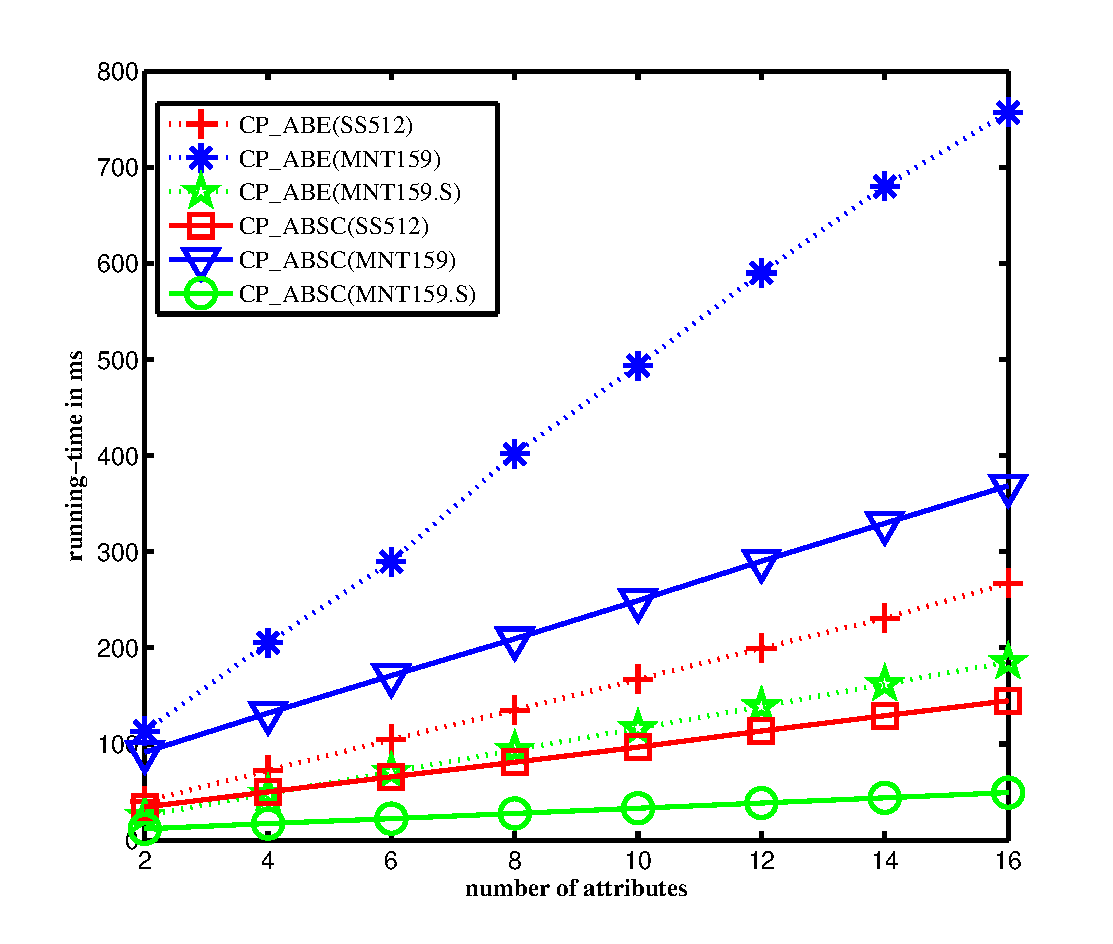
\includegraphics[width=8cm]{KeyGeneration}\\
  \caption{Key generation time}\label{sec:Fig:Key Generation time}
\end{figure}
%
%
\begin{figure}[!htp]\centering
  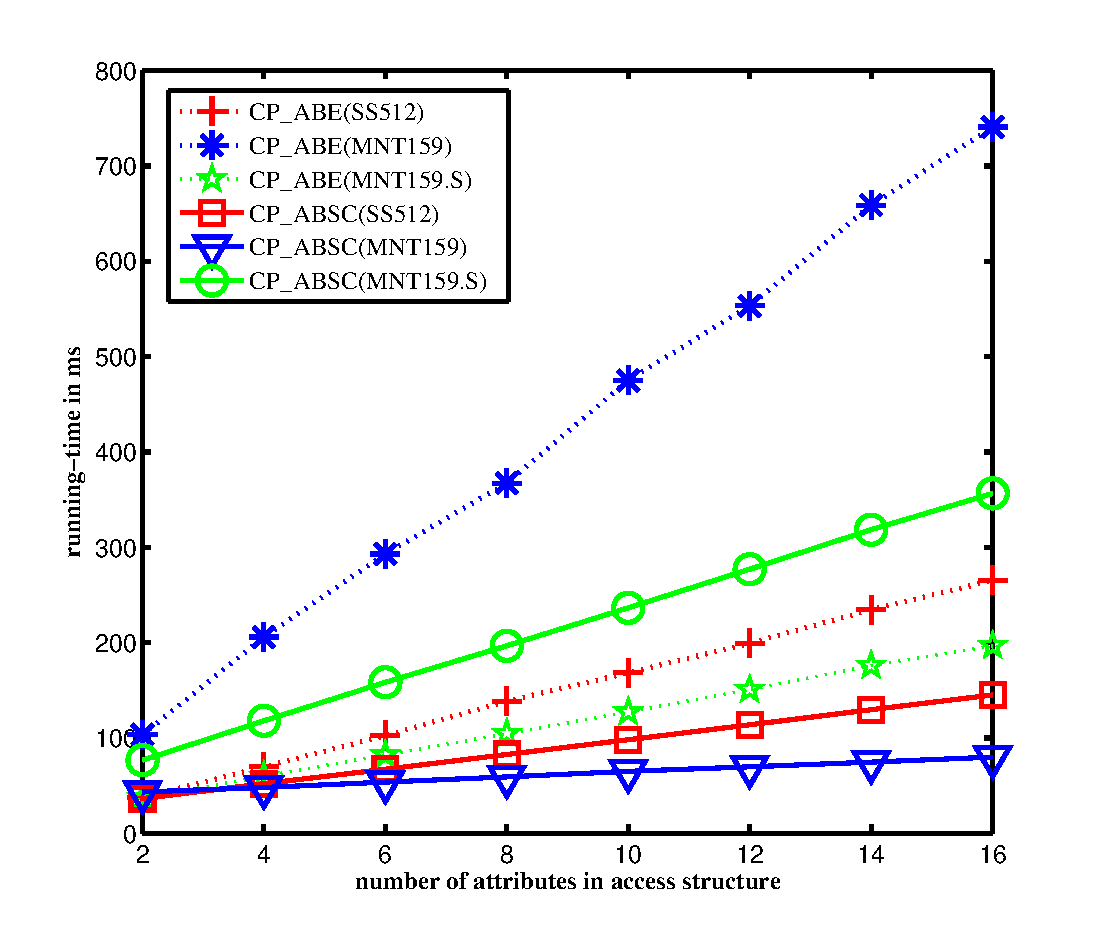
\includegraphics[width=8cm]{Encryption}\\
  \caption{Encryption time} \label{sec:Fig:Encryption time}
\end{figure}

\begin{figure}[!htp]
\centering
 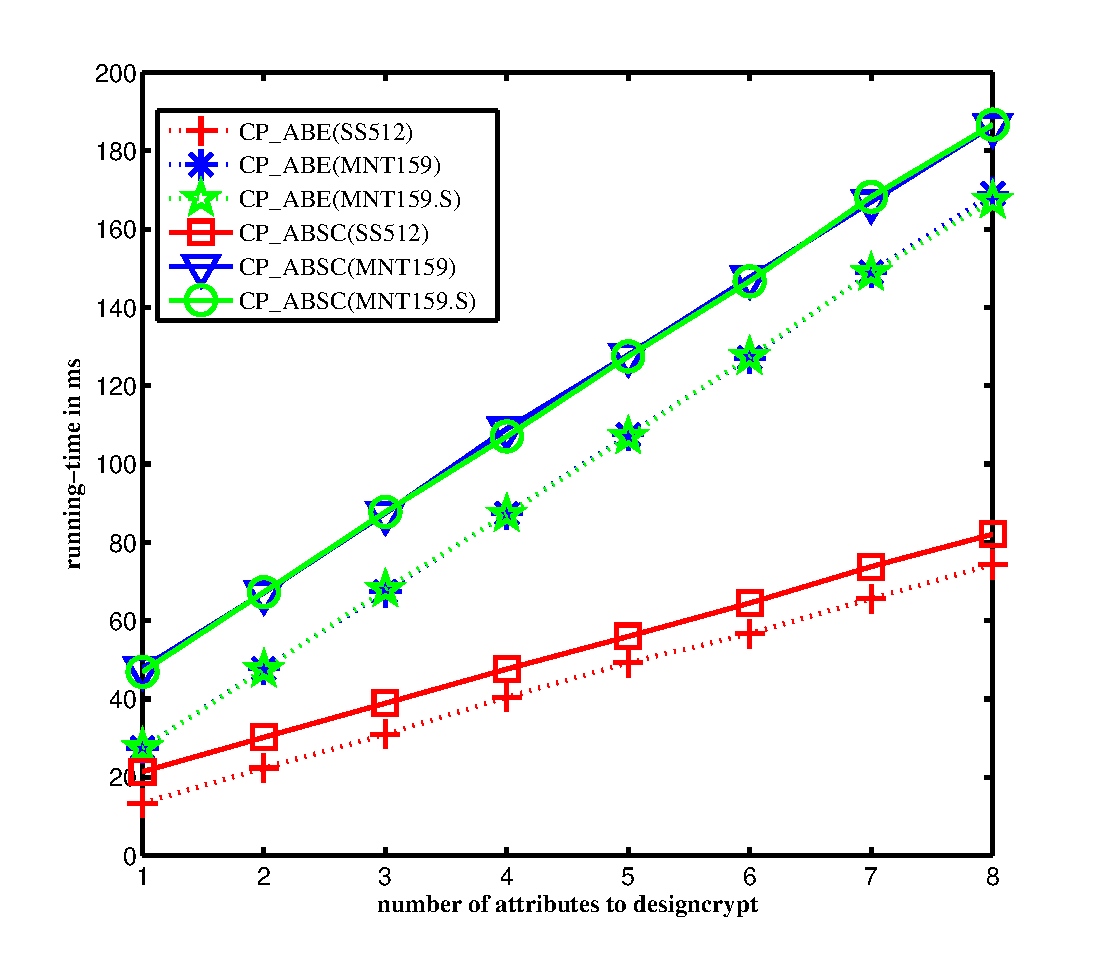
\includegraphics[width=8cm]{decryption}\\
 \centering \caption{Decryption time}\label{sec:Fig:Decryption time}
\end{figure}


%\begin{figure*}[t]\centering
%\begin{minipage}[t]{0.3\linewidth}
%\centering
%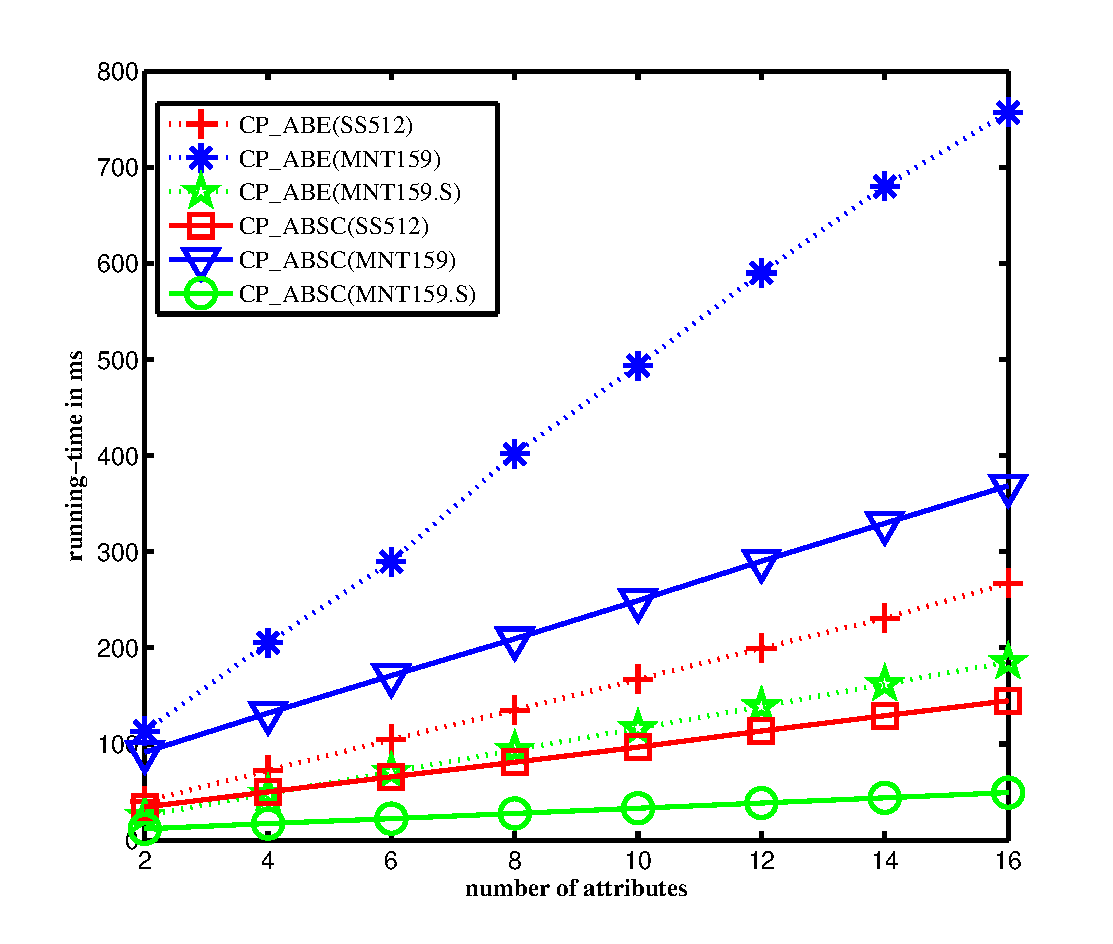
\includegraphics[height=38mm]{KeyGeneration}
%\caption{Key generation time} \label{sec:Fig:Key Generation time}
%\end{minipage}
%\hspace{4mm}
%\begin{minipage}[t]{0.3\linewidth}
%\centering
%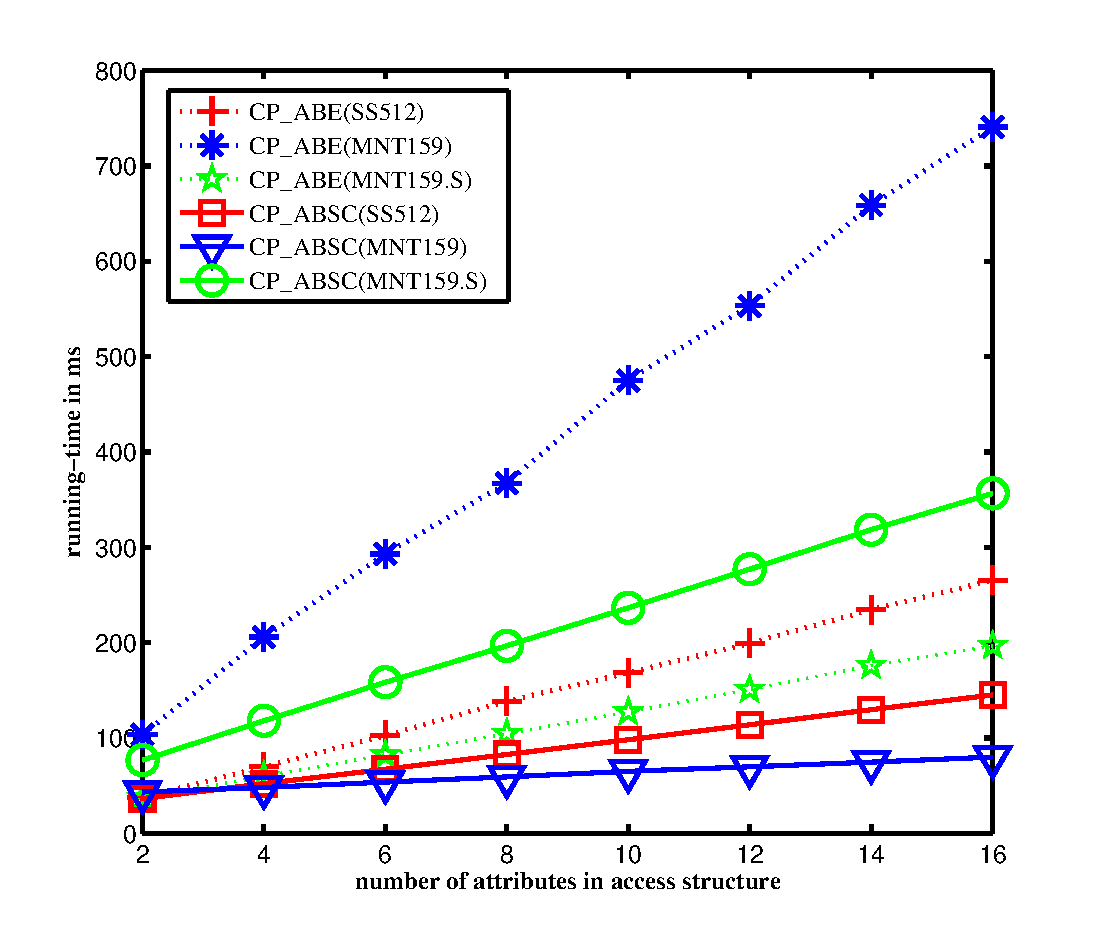
\includegraphics[height=38mm]{Encryption}
%\caption{Encryption time} \label{sec:Fig:Encryption time}
%\end{minipage}
%\hspace{4mm}
%\begin{minipage}[t]{0.3\linewidth}
%\centering
%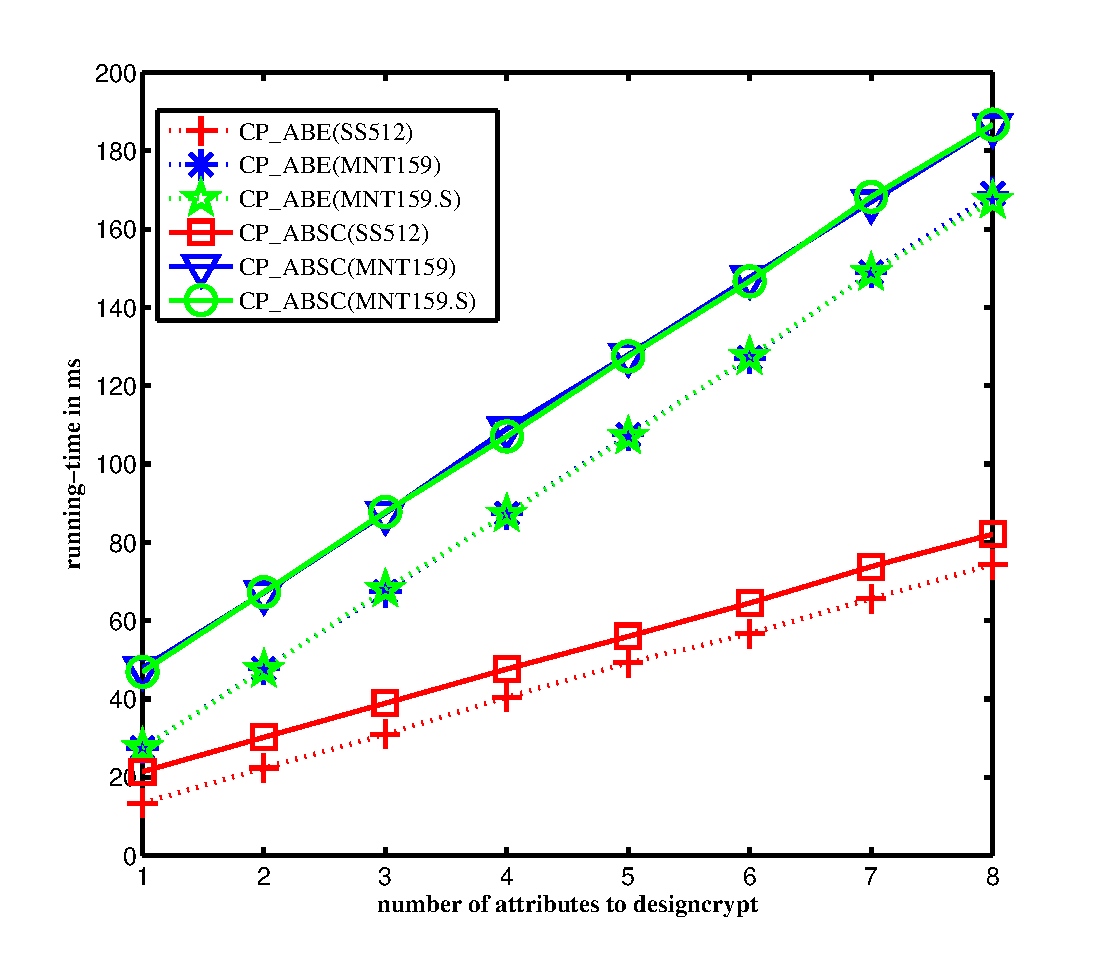
\includegraphics[height=38mm]{decryption}
%\caption{Decryption time} \label{sec:Fig:Decryption time}
%\end{minipage}
%\end{figure*}

%\begin{figure}[htp!]\centering
%  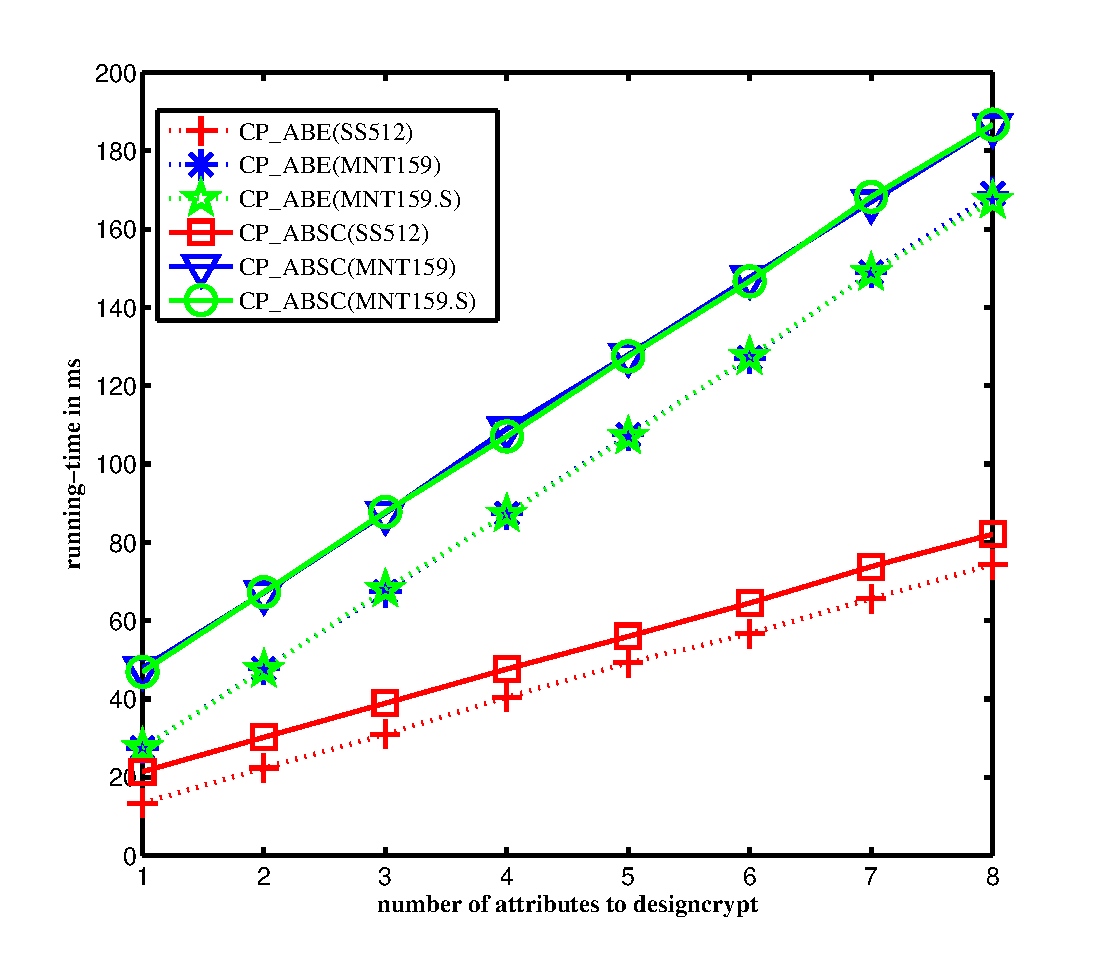
\includegraphics[height=45mm]{decryption}\\
%  \caption{Decryption time} \label{sec:Fig:Decryption time}
%\end{figure}

%====================
\emph{Forgery}: An adversary who wishes to forge the signcryption of a legal user must possess the user's signing key. An adversary cannot infer the signing key $K_{sign}$ or the root node of the access tree $T$ because the random number $r$ for each attribute in $S$  (In Algorithm \ref{alg:KeyGeneration}) and the $s$ for the root of $T$ (In Algorithm \ref{alg:Encryption}) are chosen randomly and secretly. An adversary cannot create a new, valid ciphertext from other user's ciphertexts.  If the adversary changes the ciphertext of a message, the receiver can verify that the ciphertext is illegal by Algorithm \ref{alg:decryption}. The section above on collusion shows that colluding with other users to forge a ciphertext can not succeed. Thus we claim that our proposed scheme is unforgeable. % under chosen message attacks.
\vspace{-3mm}
%====================
\emph{Confidentiality}: Decryption requires the knowledge of $e(g_1,g_2)^{\alpha s}$.  The decryption procedure takes the same idea as that of CP\_ABE \cite{bethencourt2007ciphertext}, and thus CP\_ABSC has the same security strength as that of the CP\_ABE. The designcryption requires the knowledge of $\delta=e(C,g_2)^\zeta$. For a passive adversary, the available information is $CT_{sign}$. It is difficult to get $s$ from  the $W$ in $CT_{sign}$ since it is difficult to compute the discrete logarithm problem. Even if the adversary constructs the bilinear mapping $e$ via $C$ and the public parameter $g_2$ to obtain $e(C,g_2)$,  it can not get $\zeta$, which is randomly chosen by the signcryptor. The adversary may try to get $\zeta$ from $\psi$, but it has to get the $K_{sign}$ first. Even if the $K_{sign}$ is compromised, the adversary still can't get $\zeta$ from $\psi$ due to the difficulty of computing the discrete logarithm problem. Given the discussion above and the fact that CP\_ABE is proven secure under chosen-ciphertext attacks, our scheme is secure under chosen-ciphertext attacks too.

\vspace{-2mm}
\subsubsection{Efficiency and Cost Analysis}\label{sec:performance analysis}

In this subsection, we present a quantitative performance study on CP\_ABSC in terms of computational cost.


Our scheme CP\_ABSC does not incur a high computational cost in Key Generation, SignCryption, and DeSignCryption compared to CP\_ABE. Table \ref{table:comparison computation cost between CP-ABE and our scheme} reports the amount of operations performed by CP\_ABE and CP\_ABSC. The notations are explained as follows: $n$ is the number of attributes a user holds, $k$ is the number of leaf nodes in the access tree $T$, and $k^\prime$ is the number of attributes a user possesses. The term $\Gone$ denotes an exponent operation in $\Gone$ group, and the same definitions hold for $\Gtwo$ and $\Gthree$. $H_{\Gone}$ means hashing an attribute string or message into an element in $\Gone$, and $H_{\Gtwo}$ is defined similarly.

Starting with Key Generation, as described in Algorithm \ref{alg:KeyGeneration}, there is $2n+5$ exponent operations in $\mathbb{G}_2$, which includes 5 exponent operations $\{g_2^{r_{en}}, g_2^{\beta}, g_2^{r_{sn}}, D_{en}, K_{sign}\}$, and $2n$ exponent operations $\{D_j, D_j^\prime\}$. In CP\_ABE\cite{bethencourt2007ciphertext},  the total operations is $n\Gone + (n+2)\Gtwo + nH_{\Gtwo}$.

Moving next to the Signcryption in Algorithm \ref{alg:Encryption}, there are $2k+2$ exponent operations in group $\mathbb{G}_1$ and 2 exponent operations in group $\mathbb{G}_2$. Additionally, there are $2$ map operations and 2 pairing. The combined overhead is thus $(2k+2)\Gone + 2\Gtwo + 2\Gthree + 2$ (pairings). Similarly, in CP\_ABE, the total operation is $(k+1)\Gone + k\Gtwo + 1\Gthree + kH_{\Gtwo}$.

For Designcryption (in Algorithm \ref{alg:decryption}),  there are $(2k^\prime+3)$ (pairings) operations. In CP\_ABE, there are $(2k^\prime+1)$ (pairings) operations.

We run the experiment with Ubuntu 12.04 running as a VM on a MACBook Air with one 1.8GHz core and 1GB memory. The implementation uses a Python library called Charm-crypto \cite{akinyele2013charm}, which is a framework used to prototype advanced cryptosystems such as IBE and IBS (Identity-Based Signature). The core mathematical functions behind Charm are from the Stanford Pairing-Based Cryptography (PBC) library \cite{pbclibrary}, which is an open source C library that performs mathematical operations underlying pairing-based cryptosystems.

We execute the implementation under both symmetric (SS512) and asymmetric groups (MNT159 and MNT159.S), both with 80 bits of security, to compare CP\_ABE and CP\_ABSC. In SS512, the map is $\Gone \times \Gtwo \rightarrow \Gthree$, where $\Gone$ and $\Gtwo$ are the same group.  In MNT159,  the map is $\Gone \times \Gtwo \rightarrow \Gthree$, where $\Gone$ and $\Gtwo$ are different groups, and $\Gtwo$ and $\Gthree$ are extension groups of $\Gone$. The elements in $\Gtwo$ and $\Gthree$ are longer than those in $\Gone$. The longer the element, the larger the computational cost in exponential operations. In MNT159.S, we swapped the $\Gone$ and $\Gtwo$ group so that most of the key generation operations are in $\Gone$ instead of  $\Gtwo$.

Table \ref{table:charmBenchmark} lists the run time of each operation and function in SS512 and MNT159. One can see that some operations are more efficient in SS512 than in MNT159 while others are the opposite. For example, the operations $H_{\Gone}$ and $\Gone$ have less run time in MNT159 than in SS512 but the operations of $\Gtwo$ and $H_{\Gtwo}$ have less runtime in SS512 than in MNT159. %. An exponent operation of $\Gone$ in MNT159 takes 1.12 ms, and the $H_{\Gone}$ takes just 0.1ms.

The performance analysis compares the efficiency and computational cost between CP\_ABSC and CP\_ABE  in terms of Key Generation, Signcryption/Encryption, and Designcryption/Decryption. The results are reported in Figures~\ref{sec:Fig:Key Generation time}-\ref{sec:Fig:Decryption time}.


Figure \ref{sec:Fig:Key Generation time} shows the run times of Key Generation. MNT159.S has the best performance since we swapped $\Gone$ and $\Gtwo$ and most of the operations are in $\Gone$ after the swap.

Figure \ref{sec:Fig:Encryption time} reports the encryption run times. The run time in CP\_ABE and that in our scheme CP\_ABSC is almost linear with respect to the number of leaf nodes in the access policy. The polynomial operation at leaf nodes does not significantly contribute to the run time. Comparing the run time between CP\_ABE encryption and CP\_ABSC signcryption, one can see that our scheme costs less time than CP\_ABE because we don't need to compute $H_{\Gtwo}$.

%Compared to the encryption only scheme, signcryption adds new functionality (signature). Note that with the current implementation of the Charm library, our scheme has less computational cost than CP\_ABE.

Figure \ref{sec:Fig:Decryption time} illustrates the run times of decryption. Our scheme is slightly higher than that of CP\_ABE due to the fact that we add the signature verification process. However, because the computational cost of ABE is more expensive as the number of attributes increases, the cost of signature verification is relatively trivial in practice.

Considering all three processes of KeyGeneration, SignCryption, and DeSignCryption, MNT159.S has considerably better performance than MNT159. We recommend executing the schemes in asymmetric groups and swapping $\Gone$ and $\Gtwo$ to gain a better performance.

Due to space limitation, we omit the part of comparison between the proposed scheme and Attribute based signature, which will be included in the extended version.

In summary, the run time is predictable for key generation and encryption in our scheme and is correlated with the number of attributes. Comparing the run times of key generation, encryption, and decryption between CP\_ABE and our scheme CP\_ABSC, the run times of our scheme is a little higher than CP\_ABE for some cases. However, considering that our scheme combines encryption and signature, CP\_ABSC is feasible and more desirable than the encryption-only CP\_ABE.


   \newpage
   \begin{singlespace}
   \section{Achieving Privacy Preservation and Billing via Delayed Information Release}
   \end{singlespace}

   \subsection{Motivation and Problem Formulation} \label{Sec:motivation:problem:formulation}

In this section, we first describe two real world applications to motivate our problem formulation. Then we present the challenges to tackle our problem and summarize the technical approaches employed in our scheme.

\subsubsection{Privacy-Preserving Smart Metering}


A smart metering system, as illustrated in Fig.~\ref{sec:Fig1:Smart_Grid_Architecture1},  typically consists of smart meters that collect electricity usage data at the granularity of millisecond to minute and transfer the data in realtime to utility companies. Smart meters play a critical rule in remotely collecting fine-grained energy usage data that can be used by grid operators to perform statistical analysis for effective consumption forecasting and profiling, load balancing, and demand/supply matching. Nevertheless, recent research \cite{anderson2010security,garcia2011privacy, bauer2009recognizing, hart1992nonintrusive, hart1989residential} indicates that privacy-sensitive information regarding the residents' genders, rough ages, religions, and presence/absence, etc., can be revealed by analyzing the fine-grained smart meter measurements without a paramount effort \cite{molina2010private}. Such a privacy disclosure violates the laws in many countries for safety and security concerns, and the deployment of smart meters in the Netherlands was even cancelled by the Parliament \cite{molina2010private}.

To preserve the meter owners' privacy, researchers have investigated various approaches. One mechanism is to employ a rechargeable battery to disguise the appliance loads such that the meter measurements can be maintained at a stable state for a longer time \cite{ge2013preserving,kalogridis2010privacy,varodayan2011smart}. This mechanism can successfully preserve the data privacy under normal conditions at the costs of the rechargeable battery and the battery charging and discharging losses. Nevertheless, it makes the real-time energy usage statistical analysis inaccurate.  Data pseudonymization based on secret sharing \cite{Rottondi2012greencom} or two meter identities \cite{Efthymiou2010smartgridcomm} have been proposed but they can not protect privacy as the pseudonymized consumption traces can be identified by side information or anomaly detection  \cite{Jawurek2011acsac}.  Data aggregation based on crypto primitives such as homomorphic encryption \cite{paillier1999public}, secret sharing \cite{shamir1979share,hu2012verifiable}, differential privacy \cite{danezis2011differentially}, and their combinations \cite{garcia2011privacy, rottondi2013distributed}, are the most advocated approach.  A recent survey that provides a comparative study on the applications of these crypto primitives in smart metering was reported in \cite{erkin2013privacy}. Homomorphic encryption based schemes were studied in \cite{paulet2014privacy,li2010secure,erkin2012private}. Privacy-preserving data aggregation based on secret sharing and homomorphic encryption was investigated in \cite{garcia2011privacy}.  A differential privacy based scheme was examined in \cite{acs2011have}.  %However, these schemes have either high communication cost or computational cost \cite{erkin2013privacy}. Another important problem is that these schemes protect users' privacy by hiding the fine-grained personal data in the aggregated coarse-grained results, which cannot support some services (e.g. time-of-use billing) that rely on the fine-grained data.



Note that privacy-preserving data aggregation \cite{erkin2013privacy} allows grid operators to derive the aggregated result without accessing each individual measurement, at the cost of hiding fine-grained meter readings within aggregated coarse-grained results, which renders it hard, if not impossible, to support more complicated dynamic billing and statistical calculations related to load profiling and forecasting.  Moreover, such schemes typically involve high computation and communication overheads at smart meter devices due to the high complexity of the involved crypto primitives (homomorphic encryption, secret sharing, differential privacy, or their combinations), as analyzed in \cite{erkin2013privacy}. On the other hand, data aggregation makes the time-of-use payment calculation a responsibility of the aggregators or the smart meters (\cite{rial2011privacy,jawurek2011plug}), rather than the utility companies as traditional billing does, which gives stronger incentives for the customers to abuse the meters for smaller bills.  These observations motivate us to consider novel privacy preserving fine-grained smart meter data collection mechanisms that can support monthly billing by the utility companies while involving low computational overhead at the smart meter devices.

\begin{figure}[t] \centering
  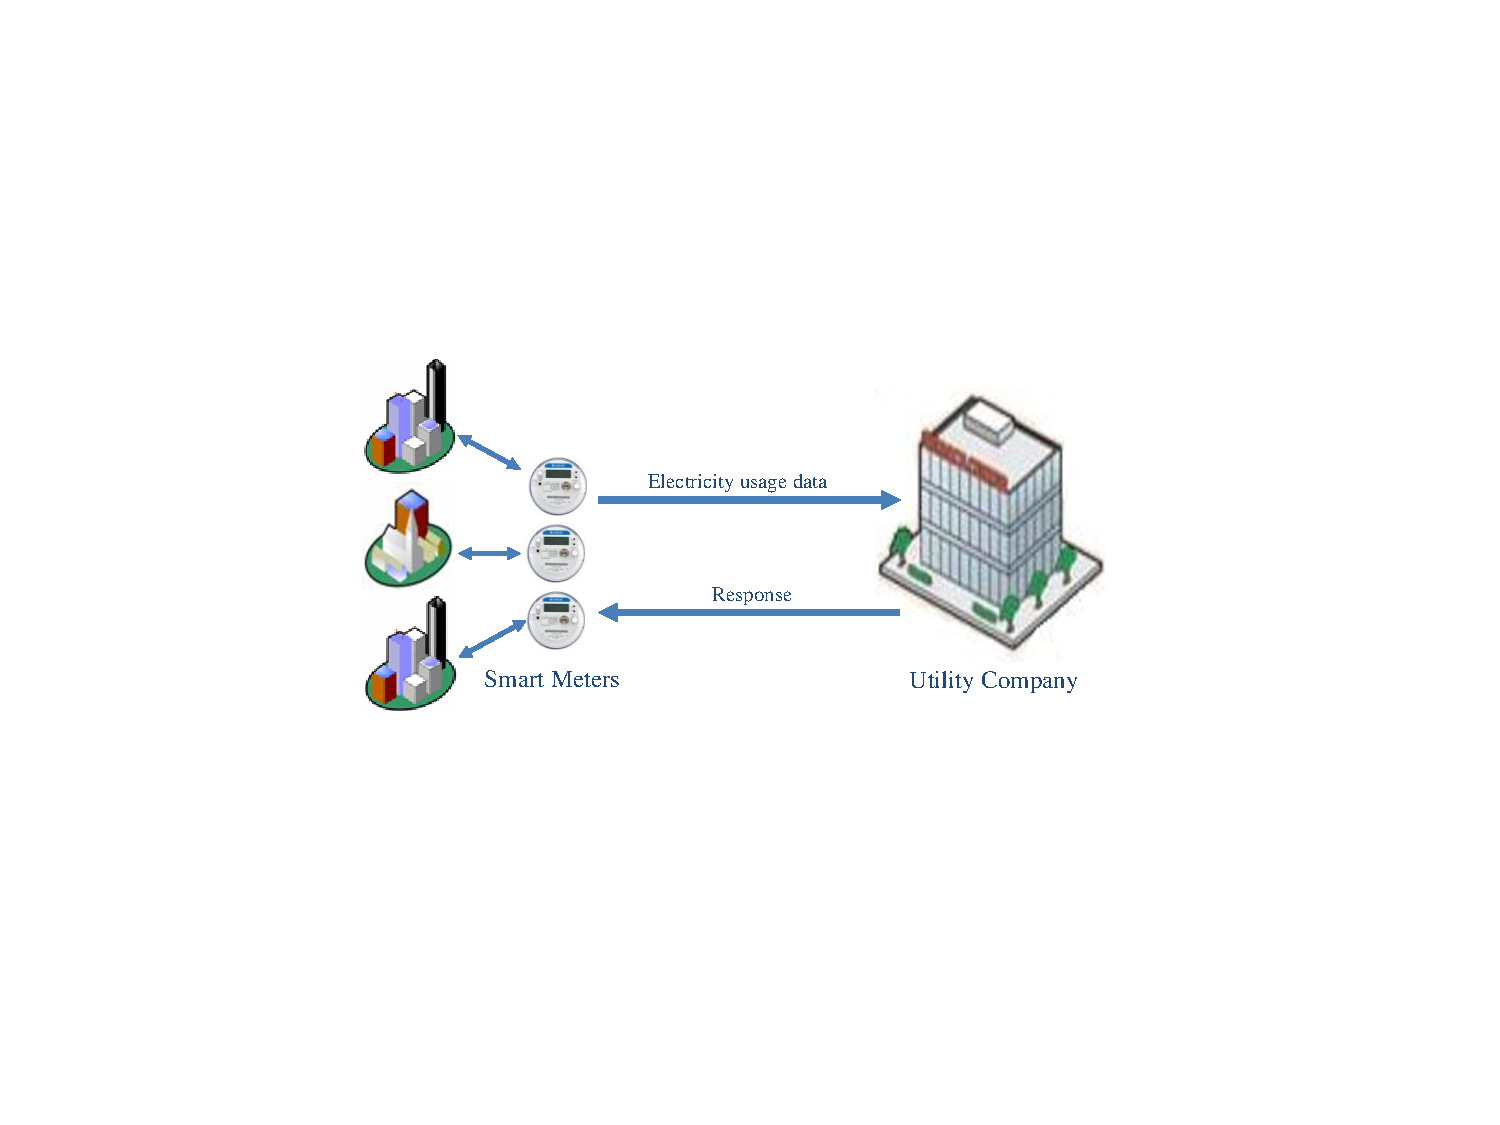
\includegraphics[width=7cm]{Smart_Grid_Architecture1}\\
  \caption{The smart metering architecture for fine-grained electricity usage data collection. } \label{sec:Fig1:Smart_Grid_Architecture1}
\end{figure}

\subsubsection{Privacy-Preserving Location-Based Services} \label{sec:lbs}

\begin{figure}[t] \centering
  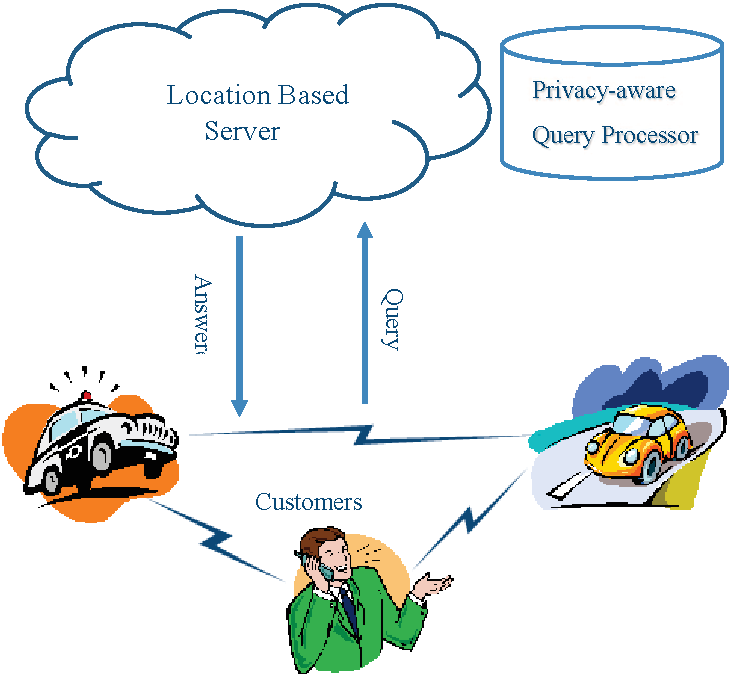
\includegraphics[width=7cm]{Location_Based_Service}\\
  \caption{A location based service system architecture. } \label{sec:Fig2:Location_Based_Service}
\end{figure}

Location based service (LBS) is another motivating example for our problem formulation. A LBS refers to an information and entertainment service that is accessible with mobile devices through mobile networks and makes use of the geographical position information of the mobile devices. Fig.~\ref{sec:Fig2:Location_Based_Service} illustrates a location based service system architecture, which includes three major entities: Location Based Server, Privacy-aware Query Processor, and Customers (clients).

LBS applications typically suffer from severe privacy and security concerns. By supplying location-based queries to the server, a client's location and possibly intention/interest can be disclosed to the server. Moreover, the server can easily trace a client as its locations are reported at each time when a query is made \cite{ma2013privacy,de2013unique}. Such private information could be exploited by malicious people to attack the clients from various aspects.

To protect client privacy in LBS, researchers have made a lot of effort.  Magkos surveyed the cryptographic primitives for privacy preservation in LBS applications \cite{magkos2011cryptographic}, which indicates that the existing approaches for privacy-preserving LBS  mainly employ crypto primitives such as zero knowledge proofs, oblivious transfer, homomorphic encryption, secret sharing, and their combinations. Most schemes \cite{mokbel2006new,jorns2007privacy,khoshgozaran2007blind} adopt a trusted third party for privacy protection, in which the client's location information is cloaked by a third party before sending to the server. Such schemes are not flexible as all communications between a client and the server must go though the trusted third party. Meanwhile, these schemes have high computation and communication overheads due to the high complexity of the crypto primitives. Vpriv \cite{popa2009vpriv} presented a protocol based on secure two party computation to compute the path functions for several driving-related problems while maintaining location privacy. This protocol is vulnerable to tracking attacks by side information because the server sees anonymous tuples with time and location information. Wen \emph{et al}.  \cite{wen2013parq} proposed a privacy-preserving range query scheme for smart grids, in which the queries are executed using cloud server's computational capabilities. The solutions in \cite{zhong2008toward} utilized the Paillier public key encryption scheme to anonymously connect with the server. In \cite{zhong2009distributed}, a scheme that can protect the privacy of the user based on the oblivious transfer primitive \cite{blake2004strong} was studied.

We notice that privacy-preserving LBS involves high computational overhead at the client side. We also notice that payment in privacy-preserving LBS, i.e, a user pays the services it has requested, is largely overlooked. These are challenging issues that motivate us to study the novel problem defined in next subsection.



\subsubsection{Problem Formulation and Challenges}

Many similar application scenarios exist in our daily life. For examples, the owner of a electronic vehicle could be traced as the vehicle is typically charged when parked; and a credit card user could release all its private information (name, card number, location, etc.) whenever the card is used, just to name a few. These applications possess the following common features:
\begin{itemize}
\item Each application involves multiple clients and one or more servers, and a client releases its private information when requesting services from the server. For examples, smart meters need to release the owners' fine-grained electricity usage data in order to take the benefits of smart grids; and a LBS user needs to submit its location information in order to get location based services.
\item The clients usually have low computation capability but require strong security and privacy protection. In our smart metering example, smart meters are relatively ``dumb'' devices but its location and collected data should be protected in order to protect the owners' privacy; in our LBS example, clients usually use smartphones to seek location based services but the location and query contents of the clients should be protected in order to protect the clients' privacy.
\item Each client needs to pay the services provided by the server, and the payment is calculated at a monthly basis by the server. For examples, the utility company should calculate the monthly bill for each smart meter owner based on the collected data and a LBS server should charge the clients for the queries they have made.
\item Each transaction between a client and a server could be modeled by a two-way message exchange that involves a query and a response. In our smart metering example, a smart meter reading can be treated as a special ``query'' for better grid services and its response could be ``null'' as fine-grained ``queries'' are submitted, and in our LBS example, the query-response model is obvious.
\end{itemize}

These observations motivate us to study the following open problem under a simple client-server model:  \emph{How to provide security and privacy protection to a client who would request services from a server and pay the service in a monthly basis?} This is a non-trivial problem that faces the following challenges:
\begin{itemize}
\item The privacy of the clients needs to be protected while the legitimacy of each request should be verifiable;

\item The confidentiality of each request should be protected;

\item The monthly bill for each client should be computable though the privacy of the client needs to be protected;

\item The transactions from different billing periods must be unlinkable though those from the same billing period must be linked together for billing purpose;

\item The computational and communication overhead must be low at the client side;

\item The solution approach much achieve nonrepudiation and accountability.

\end{itemize}

\subsubsection{Our Approach}

To tackle the challenges mentioned above, we propose a privacy preservation mechanism based on delayed information release that can not only provide the required services at low cost in the client side but also protect the clients' privacy and data confidentiality. Meanwhile monthly bills (or statement reports) can be successfully computed without releasing any information for the server to link the transactions of a client made at different billing periods. The key strategies adopted in our design can be summarized as follows:

\begin{itemize}
\item To best protect a client's privacy,  we anonymize each request based on a secret token to hide the true identify of the client; to verify the legitimacy of each anonymous request and to achieve non-repudiation and accountability, we employ group signatures. Such a strategy ensures that the server is able to verify whether a request is from a legal user registered in a group but does not know who the client is. Therefore the server can not link all the requests made by a client unless more information is available.

\item To provide confidentiality for each transaction, Rabin's public key cryptosystem, which is featured by a lightly-weighted encryption operation at the client side, is adopted to encrypt the anonymous data. This shifts the computational complexity from the client to the server, which are usually supported by computing resources such as clouds. The response from the server is protected by AES, a symmetric algorithm with low computational overhead.

\item To compute the monthly bill for each client, the token is securely released to the server (via Rabin's encryption) at the end of the billing period. A one-way hash chain seeded by the token is utilized to identify all the requests made by the client in a billing period. Each client maintains its own token and the token changes at the beginning of each billing period, to prevent the server from linking the requests made by the same client at different billing periods. Though the server can trace a client's requests made within a billing period but this happens only when the token is released to the server at the end of the billing period; other eavesdroppers have no way to link the requests of a client made within one or multiple billing periods.

\end{itemize}



%========================================================================================================================

\subsection{System Model and Security Model} \label{sec:modelsDesignGoal}

\begin{figure}[t] \centering
  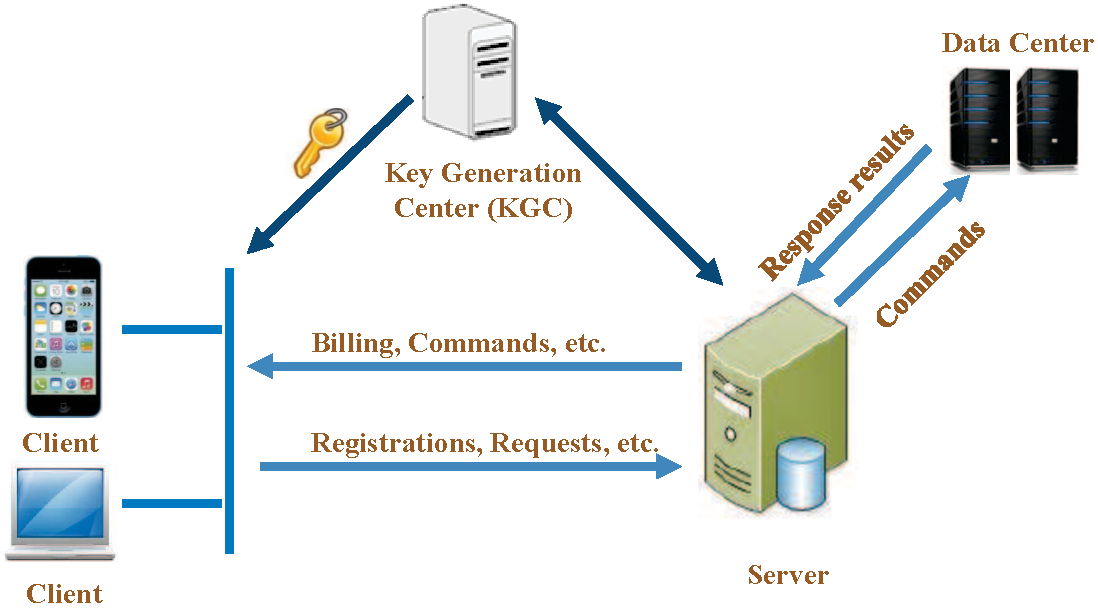
\includegraphics[width=7cm]{systemframework}\\
  \caption{A communication architecture } \label{sec:Fig1:SystemCommunication}
\end{figure}

\subsubsection{System Model}

As shown in Fig.~\ref{sec:Fig1:SystemCommunication}, our system model consists of four major entities: Key Generation Center (KGC), Client, Data center, and Server. In the following we briefly summarize the major functions of each entity.
\begin{itemize}
\item \emph{The Key Generation Center (KGC):}  KGC is used to generate and distribute keys for all the clients and  the server. KGC also takes the role of group manager. It is responsible for group formation and dispute resolution. %Because the KGC can forge the signature of a client, the KGC is assumed to no longer be trusted by the clients.

\item \emph{Client:} Each client needs to register with KGC and joins a group in order to get services from the server. During the registration and join processes, each client computes or receives from KGC its group member id and group certificate. A legitimate client should be able to get services from the server without releasing its private information. % For collect data, and send encrypted data to the server.

\item \emph{Data center:} The data center (may consist of cloud servers) is utilized to process the data for the server.

\item \emph{Server:} The server will get group information (group id and group public parameters) from KGC and will service the clients in the corresponding groups. It will generate monthly bills for the services provided to each client. The disputes between the server and a client is resolved by KGC.
\end{itemize}

\subsubsection{Security Model}
In our security model, we assume that KGC is a trusted-third-party. There is a secure channel between KGC and each client, which is used to transmit sensitive information during the registration and join operations. This secure channel is also used when disputes need to be resolved at KGC.

We consider that the following security goals need to be achieved:
%
\begin{itemize}
\item Privacy-preservation of client requests and identities. The server should be able to verify that a request is made by a legitimate client though the client identity is kept confidential; i.e, the server is able to tell that a request is made by a legal user without knowing who has made the request. Both the requests from clients and the responses from the server should be protected for confidentiality. The requests made by the same client within a billing period should be identifiable only by the server for billing purpose, but those from different billing periods should never be linked by the server to protect the client privacy.

\item Non-repudiation: If a client has made a request and serviced by the server, it can not deny this activity in later time. If the server charges a client for a request that is not made by the client, the forged services should be identifiable.

\item Accountability:  The system is recordable and traceable. When there exists any security issue or a dispute between a client and the server, the system should be able to figure out who is responsible for what.
\end{itemize}

%Based on the system and security models and our design objectives mentioned above, we intend to develop an efficient privacy-preserving scheme via delayed information release:
%
%\begin{itemize}
%\item The proposed scheme should protect the client's identity, while the client can not deny that it used the service.
%
%\item The proposed scheme should protect the privacy of the client's requests and the payments.
%
%\item The server not only provides the service for the anonymous clients, but also can caluculate the monthly bill for the anonymous clients for each billing period.
%\end{itemize}

%=====================================================================================================================================
%\section{Preliminaries}\label{sec:preliminaries}
%In this section, we provide an overview on the following cryptographic primitives: bilinear map, group signature, and the Rabin cryptosystem, which will serve as the basis for our proposed PPDIR scheme.


%\subsection{Bilinear Maps}
%
%Let $\mathbb{G}_1$ and $\mathbb{G}_2$ be two bilinear groups of prime order $q$, and $G$ be a generator of $\mathbb{G}_1$.  Our
%proposed scheme makes use of a bilinear map: $e: \mathbb{G}_1\times \mathbb{G}_1\rightarrow \mathbb{G}_2$ with the following properties:
%
%\begin{itemize}
%\item {\em Bilinear:} A map $e: \mathbb{G}_1\times \mathbb{G}_1\rightarrow \mathbb{G}_2$ is bilinear if and only if for $\forall Q\in \mathbb{G}_1$ and $\forall a, b \in \mathbb{Z}^*_q$, we have $e(aG,bQ)=e(G,Q)^{ab}$. Here $\mathbb{Z}_q^{\ast} = \{1, \ldots, q-1\}$ is the Galois field of order $q$.
%
%\item {\em Non-degeneracy:} The generator $G$ satisfies $e(G,Q)\neq 1$ for $\forall Q\in\mathbb{G}_1$.
%
%\item {\em Computability:} There is an efficient algorithm to compute $e(G,Q)$ for $\forall Q \in \mathbb{G}_1$.
%\end{itemize}
%
%Next we define the Gap Diffie-Hellman (DH) Group. To proceed, let's first introduce DLP, CDHP, and DDHP.
%
%\begin{itemize}
%\item \emph{Discrete Logarithm Problem (DLP)}: Given a generator $G$ and an element $Q\in\mathbb{G}_1$, DLP intends to find the integer $\alpha \in \mathbb{Z}_q$ such that $Q=\alpha G$ whenever such an integer exists.
%
%\item \emph{Computation Diffie-Hellman Problem (CDHP)}: Given $G$, $aG$, and $bG$ for $a, b \in \mathbb{Z}_q$, CDHP computes $abG$.
%
%\item Decision Diffie-Hellman Problem (DDHP): Given $G$, $aG$, $bG$, and $cG$ for $a,b,c\in \mathbb{Z}_q$, DDHP decides whether $c\equiv ab \mod q$.
%\end{itemize}
%
%We call $\mathbb{G}_1$ a Gap DH Group if DDHP can be solved in polynomial time but there is no polynomial time algorithm to solve CDHP or DLP with a non-negligible probability. Such a group can be found in supersingular elliptic curve or hyperelliptic curve over finite fields, and the bilinear pairing can be derived from the Weil or Tate parings\cite{boneh2001identity,choon2002identity}.




%====================================================================================================================================

\subsection{The Proposed Scheme}\label{sec:ProposedScheme}
In this section, we detail our scheme for Privacy Preservation and billing via Delayed Information Release (PPDIR).  At the beginning of any billing period, each client needs to select a secret token and compute a one-way hash chain seeded by the token and $H(ID)$. The token will be securely released to the server at the end of the billing period to link all requests made by the same client during the current billing period for billing purpose. Each request is anonymous, is attached with one element in the hash chain, and is signed based on our group signature scheme such that the server can verify that the request is made by a valid member belonging to certain group but it can not figure out the group member who has generated and signed the request. All the information transmitted from the client is protected by Rabin cryptosystem and the response from the server is encrypted by AES such that the computational complexity at the client side is low. Since the token will never be public, attackers can not link the requests made by the same client within the same billing period; as the token is unique for each billing period, neither attackers nor the server can link the requests made at different billing periods.


\subsubsection {Setup}\label{Sec:setup}

We assume that the server bootstraps the system. Specifically, the server first generates its private key  $\{n_1, n_2\}$ and the corresponding public key $n=n_1n_2$  based on the Rabin cryptosystem. The server keeps its private key $\{n_1, n_2\}$ and publishes its public key $n$.

KGC manages all the groups. To create a group, KGC needs to perform the following activities:
\begin{itemize}
\item KGC chooses a cyclic additive group $\mathbb{G}_1$ (which is a Gap DH group) of prime order $q$, which is generated by $G$, and a cyclic multiplicative group $\mathbb{G}_2$ with the same order $q$.

\item  KGC selects one secure symmetric encryption function such as AES, denoted by $Enc()$, and three secure cryptographic hash functions $\{H, H_1, H_2\}$, where $H, H_1: \{0,1\}^*\longrightarrow \mathbb{Z}_q^{\ast}$ and $H_2: \{0,1\}^*\longrightarrow \mathbb{G}_1$, here $\mathbb{Z}_q^{\ast} = \{1, \ldots, q-1\}$.

\item KGC chooses a random master key $s \in \mathbb{Z}_q^*$ and computes a public key $P=sG$.
\end{itemize}

KGC publishes the following public parameters for the newly-created group $\mathcal{G}$:
\begin{equation}
params=\{\mathbb{G}_1, \mathbb{G}_2, e, q, G, P, H, H_1, H_2\}.
\end{equation}
where the bilinear pairing is a map $e: \mathbb{G}_1\times \mathbb{G}_1\longrightarrow \mathbb{G}_2$.
KGC keeps the master secret key $s$.

\subsubsection{Registration and Join}\label{sec:sec:Registration_Join}
When a client with identity $ID$ registers with KGC, the following two steps need to be performed:
\begin{enumerate}
 \item The client randomly chooses an integer $r \in \mathbb{Z}_q^{\ast}$ as its private key, and sends $rG$ to KGC via a secure channel.

 \item KGC calculates $S_1=sH_2(H(ID), rG)$, and sends it to the client via a secure channel.
\end{enumerate}
The client's private key pair is $\{r, S_1\}$, and its public key is $H(ID)$. Note that we use $H(ID)$ instead of the $ID$ itself as the public key of the client and the true $ID$ of the client in our system is never released for privacy protection.


Here we assume a secure channel exists between KGC and each client such that the information exchanged during client registration can be protected. This assumption is reasonable as a client needs to be authenticated during registration in many practical applications that consider security a big issue.

After registration, the client can choose a group to join. Note that we separate the registration and join operations because a client may register with KGC but does not choose any group to join.  The join process is outlined as follows:
\begin{enumerate}
 \item The client chooses a random number $x \in Z_q^{\ast}$, and sends $\{rG, xG, rxG, S_1\}$ to KGC requesting to join the group $\mathcal{G}$ with public parameters $params=\{\mathbb{G}_1, \mathbb{G}_2, e, q, G, P, H, H_1, H_2\}$.

 \item KGC verifies $e(rxG, G)\overset{?}{=}e(xG, rG)$ to check whether the client is a valid registered member of group $\mathcal{G}$. If true, KGC sends $S_2=sH_2(H(ID),rxG)$ to the client via the secure channel; otherwise, the join request is declined.
\end{enumerate}

Note that $x$ is a private parameter selected by the client to bind itself with the group to join.
The tuple $\{rG, xG, rxG, ID\}$ is used as the identity of the client in the group; thus it is added to the group member list. The client's member certificate is comprised of $\{S_2, rxG\}$ and its private signing key pair is $\{x, rx\}$.

A client does not need to register with the server as long as KGC reports to the server all the groups that may request services from the server. Each group has a unique identity $\mathcal{G}$ and its public parameters should be certified by KGC. Whenever a client sends an anonymous request to the server, the identity of the group it joins instead of its true identity should be included in order for the server to identify which group it belongs to while keeping its true identity confidential.

\subsubsection{Group Signature}\label{sec:signprotocol}
We propose a group signing procedure in this subsection in order for the server to ensure the authenticity of the client's request, i.e., to verify that the request is signed by a valid member of a group. Although our signature method is motivated by  \cite{chen2003new}, it possesses a nice property that significantly differ itself from the one in  \cite{chen2003new}. Let $M$ be the request message to be signed by a client. The following two steps outline the signing procedure.

\begin{enumerate}
\item  The client randomly selects two numbers ${k_1, k_2} \in \mathbb{Z}_q $;

\item  The client employs its two signing keys $\{x, rx\}$ and the member certificate $\{rxG,S_2\}$ to sign the request $M$ as follows:
\begin{itemize}
\item $U=k_1rxG$;
\item $V=(q-k_1)xG$;
\item $Y=rH_2(H(M), U+V)$;
\item $\delta=rxH_2(H(M), U+V)$;
\item $R=k_2H_2(H(ID), rxG)$;
\item $l=H_1(H(M), U+V+R)$;
\item $W=lk_2S_2+k_1rxH_2(H(M), U+V+R)$
\end{itemize}
\end{enumerate}
The signature on $M$ is the tuple $ GSign=\{U, V, Y, \delta, R, W\}$.

Our signature scheme proposed above allows a single signing key pair to be used to sign as many messages as a client would like to do because two random numbers $\{k_1, k_2\}$ are actually utilized to compute the signature for each message, while the one in \cite{chen2003new} requires a unique signing key pair for each message. This advantage can help conserve the storage space and decrease the overhead of managing a large number of signing key pairs, which is particularly useful when a client needs to sign many requests. In Subsection~\ref{sec:sec:security_strength}, we will prove that our signature scheme still possesses the security properties required by group signatures.



\subsubsection{Encryption}\label{sec:sec:encryption}
To preserve a client's privacy, we must prevent attackers from linking multiple transactions (each transaction consists of a client request and the corresponding response from the server) made by the same client within one billing period or across multiple billing periods. To achieve this objective, we employ hash chains and secret tokens to create different IDs for each transaction during each billing period. This method ensures that an attacker can not trace a client even though it intercepts all the messages destined to or originated from the client. The basic idea is outlined as follows.

For each billing period $T$, we require the client to randomly choose a token $\tau$ and compute its initial seed $h^0$: $h^0=H(H(ID)||\tau||T)$. A one-way hash chain $h^j=H(h^{j-1},\tau)$ is also computed, with $j=1, 2, \cdots,$ and $h^j$ to be used by the $j^{th}$ request of the client in the current billing period $T$. Note that $\tau$ must be unique for each billing period but the client's identity $ID$ does not need to be changed as it is never released.

To make an anonymous and privacy-preserving request to the server, the client performs the following steps based on Rabin encryption:

 \begin{enumerate}
 \item  For the $j^{th}$ request $M$, the client chooses a session key $k^j$ based on $AES$.
 \item  The client computes $M_1$ and $R$, where $M_1=M||GSign||h^j||k^j$,  and $R$ is the last 128-bits of $M$. Then the client computes $\overline{M}=M_1*2^{128}+R$. Note that $R$ provides the required redundancy to facilitate the Rabin decryption.

 \item  The client employs the server's public key to encrypt $\overline{M}$ based on the Rabin encryption:
 \begin{equation}
Rabin\_C=Rabin\_Enc(\overline{M}).
\end{equation}

 \item   The client sends the ciphertext \emph{Rabin\_C} to the server.
 \end{enumerate}

 This procedure provides a session key $k^j$ for the $j^{th}$ request in the current billing period, and $k^j$ will be used by the server to encrypt the response based on AES if the client's request is validated. We choose AES to protect the session as it is strong enough while involving a low computational cost for both encryption and decryption.

\subsubsection {Decryption and Verification}\label{sec:sec:decryption}

When the server receives \emph{Rabin\_C}, it decrypts the ciphertext using its private key $(n_1, n_2)$, and verifies the group signature $GSign$. The decryption and verification procedure is outlined as follows:
\begin{enumerate}
\item  The server decrypts \emph{Rabin\_C} and gets four decrypted messages $\{ \overline{M_1'}, \overline{M_2'}, \overline{M_3'}, \overline{M_4'}\}$.

\item  The server identifies the message $\overline{M}$ that possesses the redundancy (the $R$ part). It then recovers the original message by computing $M''=\frac{\overline{M}-R}{2^{128}}$, which consists of  $\{M', GSign, h^{j}, k^j \}$
\item The server calculates $l'=H_1(H(M'), U+V+R)$.
\item  The server verifies the following equations:
\begin{equation}
 e(G, \delta )=e(V, Y)\cdot e(U, H_2(H(M'),U+V)) \label{equ:WP2}
\end{equation}
\begin{equation}
 e(G, W)=e(U, H_2(H(M'), U+V+R))\cdot e(P, R)^{l'} \label{equ:WP}
\end{equation}
\end{enumerate}

If  (\ref{equ:WP2}) and (\ref{equ:WP}) hold, the client's request is accepted by the server; otherwise, the server declines the request as the client is not verified.

Note that the server is able to verify  whether the client is a legal registered user belonging to a certain group according to (\ref{equ:WP2}) and (\ref{equ:WP}) but it does not know who requests the service.  The security properties of this signature verification scheme is analyzed in Section \ref{sec:sec:security_strength}.

\subsubsection{Response}\label{sec:sec:response}
 After the server verifies that the client is legal, it sends a Response of Request (RoR) to the client:
 %
\begin{enumerate}
\item  The server creates its response, encrypts it with the session key $k^j$ based on AES: $Res=Enc_{k^j}(RoR)$, and then sends $Res$ to the client.
\item  The server computes the payment $b_j$ for the current service(s), and stores the request $M$,  the signature $GSign$, the response $RoR$, the bill $b_j$, and the hash value $h^j$ for billing purpose and accountability guarantee.
\end{enumerate}

After receiving $Res$, the client decrypts it to obtain the response using session key $k^j$. %Note that How can the server send encrypted response to the anonymous

\subsubsection {Delayed Information Release}\label{sec:sec:delayed}

 At the end of the current billing period, the client is required to securely release the secret token $\tau$ and the hash chain seed $h^0$. This process is secured by the Rabin encryption based on the procedure outlined in Section~\ref{sec:sec:encryption}. Let $k$ be the session key selected by the client for information release and billing purpose.

When the server receives the released information,  it decrypts to get the token $\tau$ and the session key $k$. Then it computes the hash chain according to the token $\tau$ and $h^0$. Based on the hash chain, the server can link all the requests made by the same client during the current billing period, and calculates the client's payments $pyt$. Then the server sends the bill to the client based on the following two steps:
\begin{enumerate}
\item  The server encrypts the client's payment $pyt$ using the client's session key $k$ : $Pay=Enc_{k}(pyt)$.

\item  The server sends $Pay$ to the client.
\end{enumerate}

When the client obtains $Pay$, it decrypts the message to obtain the payment $pyt$, and pay the bill.
%
The client's detailed statement report can also be released, by following the same procedure.



%===========================================================================================================================================

\subsection{Security Analysis}\label{sec:SecurityAnalysis}
In this section, we investigate the security properties of our group signature scheme, and analyze the security strength of PPDIR in guaranteeing client privacy protection, non-repudiation, accountability, and authentication.


\subsubsection{The Security Properties of Our Group Signature Scheme}\label{sec:sec:security_strength}
In this section, we prove the security strength of the group signature scheme proposed in Section~\ref{sec:signprotocol}. Note that $\mathbb{G}_1$ is a Gap DH group in our scheme.

\begin{theorem}\label{sec:sec:security_resist_fake}
If an adversary can forge a valid signature, then the adversary should be able to solve DLP in $\mathbb{G}_1$ with a non-negligible probability.
\end{theorem}
\begin{proof} For contradiction we assume that an adversary can forge a valid signature. Then this signature must be able to pass the verification  check established by equations \eqref{equ:WP2} and \eqref{equ:WP}. Considering \eqref{equ:WP}. The right-hand side of \eqref{equ:WP} can be transformed to $e(U, H_2(H(M), U+V+R))\cdot e(P, R)^{l}=e(U, H_2(H(M), U+V+R))\cdot e(sG, R)^{l}$ while the left-hand side of \eqref{equ:WP} is $e(G, W)$. Comparing the two sides, one can see that if  \eqref{equ:WP} is correctly established, the computation of $W$ must involve $s$, which means that the attacker can obtain the master key $s$ from the public key $P=sG$. This implies that the attacker can solve \emph{DLP} in $\mathbb{G}_1$ by computing $s$ from $sG$, which further implies that the attacker can solve the discrete logarithm problem in $\mathbb{G}_1$. % which contradicts the fact that \emph{DLP} is \emph{NP}-hard problem.
Therefore no adversary can forge a valid signature with a non-negligible probability.
\end{proof}


\begin{theorem}\label{sec:sec:theorem:No_Group_member}
No group member (client) can impersonate and sign on behalf of any other group member with a non-negligible probability.
\end{theorem}
\begin{proof} Consider the following impersonation attacks:

\textbf{Case 1}: The attacker does not collude with KGC.

Assume that a client with identity $ID_j$ is the attacker who intends to impersonate another client with identity $ID_i$ to sign $ID_i$'s request $M$. In order to forge a valid signature for $M$ that can pass the verification check, the attacker needs to choose appropriate values of $U$, $V$, $Y$, $\delta$, $R$, $W$ such that  \eqref{equ:WP2} and \eqref{equ:WP} can hold. Because $G$ and $P$ are public, the attacker must establish a valid relationship between $\{G, P\}$ and $\{U, V, Y, \delta, R, W\}$. Considering the two side of  \eqref{equ:WP2} and \eqref{equ:WP}, one can see that it is easy for the attacker to forge a signature when $U=V=G$ or $U=V=P$, which reduces the difficulty to establish a valid relationship between $\{G, P\}$ and $\{U, V, Y, \delta, R, W\}$ as the attacker only needs to consider the relationship between $\{G, P\}$ and $\{Y, \delta, R, W\}$.
\begin{itemize}
\item When the attacker chooses $U=V=G$:

The right-hand side of \eqref{equ:WP2} can be transformed to:
\begin{eqnarray} \label{equ:WP2_right3}
&&e(V, Y)\cdot e(U, H_2(H(M), U+V)) \nonumber\\
&=&e(G, Y)\cdot e(G, H_2(H(M),U+V)) \nonumber\\
&=&e(G, Y+H_2(H(M), U+V))
\end{eqnarray}
Comparing the left-hand side of \eqref{equ:WP2} and the right-hand side of \eqref{equ:WP2_right3}, one can see that the attacker can pass the verification check \eqref{equ:WP2} when  $\delta=Y+H_2(H(M), U+V)$, where $Y$ can be selected randomly by the attacker.

But it is not easy for the forged signature to pass the verification check \eqref{equ:WP}, as the attacker does not know the certificate component $S_2$ of  $ID_i$. %, it determines $W$ via the verification equation \eqref{equ:WP}.
%
The right-hand side of \eqref{equ:WP} can be equivalently transformed to:
\begin{eqnarray} \label{equ:WP_right3}
&&e(U, H_2(H(M), U+V))\cdot e(P, R)^l \nonumber\\
&&=e(G, H_2(H(M),U+V))\cdot e(sG, R)^l \nonumber\\
&&=e(G, H_2(H(M),U+V)) \cdot e(G, lsR) \nonumber\\
&&=e(G, lsR+H_2(H(M),U+V))
\end{eqnarray}
Comparing the left-hand side of \eqref{equ:WP} and  the right-hand side of \eqref{equ:WP_right3}, one can see that the forged signature can pass the verification check \eqref{equ:WP} when $W=lsR+H_2(H(M),U+V)$. Because the attacker does not know the master key $s$, which is held by KGC, the attacker can only brute-force $W$ to establish $W=lsR+H_2(H(M),U+V)$, which can succeed with a probability $1/(q-1)$. %Because $q$ is a very large prime number, we claim that in this case the probability of successfully impersonating a legal group member is non-negligible.

\item When the attacker chooses $U=V=P$:

The right-hand side of \eqref{equ:WP2} can be equivalently transformed to
\begin{eqnarray} \label{equ:WP2_right4}
&&e(V, Y)\cdot e(U, H_2(H(M), U+V)) \nonumber\\
&=&e(sG, Y)\cdot e(sG, H_2(H(M),U+V)) \nonumber\\
&=&e(G, s(Y+H_2(H(M), U+V)))
\end{eqnarray}
Comparing the left-hand side of \eqref{equ:WP2} and the right-hand side of \eqref{equ:WP2_right4}, one can see that the forged signature can pass the verification check \eqref{equ:WP2} only when $\delta=s(Y+H_2(H(M), U+V))$. However, the attacker can not compute $\delta=s(Y+H_2(H(M), U+V))$ because it does not know the master key $s$. Brute-forcing all possible values of $\delta$ has a success probability of only $1/(q-1)$ to establish $\delta=s(Y+H_2(H(M), U+V))$.

Now we consider whether the attacker can pass the verification check \eqref{equ:WP}. The right-hand side of \eqref{equ:WP} can be transformed to
\begin{eqnarray} \label{equ:WP_right4}
&&e(U, H_2(H(M), U+V))\cdot e(P, R)^l \nonumber\\
&&=e(sG, H_2(H(M),U+V))\cdot e(sG, R)^l \nonumber\\
&&=e(G, sH_2(H(M),U+V))\cdot e(G,lsR) \nonumber\\
&&=e(G, s(lR+H_2(H(M),U+V)))
\end{eqnarray}
Comparing the left-hand side of \eqref{equ:WP} and  the right-hand side of \eqref{equ:WP_right4}, one can see that the forged signature can pass \eqref{equ:WP} only when $W=s(lR+H_2(H(M),U+V))$. Because the attacker does not know the master key $s$, it can not establish $W=lsR+H_2(H(M),U+V)$;  Brute-forcing all possible values of $W$ has a success probability of only $1/(q-1)$.

Therefore we claim that in this case the attacker can forge a valid group signature with a probability at most $1/(q-1)^2$ as \eqref{equ:WP2} and \eqref{equ:WP} must simultaneously hold.
\end{itemize}

According to the above analysis, one can see that the attacker can impersonate a valid group signature with a probability at most $1/(q-1)$ as it needs to  brute-force all possible values of $\delta$ and $W$. Recall from Section \ref{Sec:setup} that $q$ is a very large prime number; therefore the probability of successfully impersonating a legal group member is negligible.


\textbf{Case 2}: The attacker colludes with KGC.

In this case, the attacker with identity $ID_j$ can obtain $\{r_iG, x_iG\}$ and the member certificate $\{S_2, r_ix_iG\}$ of an honest group member with identity $ID_i$ by colluding with KGC. The attacker chooses $k_1^\prime, k_2^{\prime}\in \mathbb{Z}_q$, $r_x, x_x\in\mathbb{Z}_q^*$, and obtains the following values:
\begin{eqnarray}
U&=&k_1^{\prime}r_ix_iG\nonumber\\
 V&=&(q-k_1^{\prime})x_iG\nonumber\\
Y&=&r_xH_2(H(M), U+V)\nonumber\\
\delta &=&r_xx_xH_2(H(M), U+V)\nonumber\\
R&=&k_2^{\prime}H_2(H(ID_i), r_ix_iG)\nonumber\\
l&=&H_1(H(M), U+V+R)\nonumber\\
W&=&lk_2^\prime S_2+k_1^{\prime}r_xx_xH_2(H(M), U+V+R)\nonumber
\end{eqnarray}

According to the  \eqref{equ:WP2}, we have:
%
\begin{eqnarray}\label{equ:WP2_left2}
e(G,\delta)&=&e(G, r_xx_xH_2(H(M), U+V)) \nonumber\\
&=&e(r_xx_x G, H_2(H(M), U+V))
\end{eqnarray}
%
On the other hand, the right-hand side of \eqref{equ:WP2} can be equivalently transformed to
\begin{eqnarray} \label{equ:WP2_right2}
&&e(V, Y)\cdot e(U, H_2(H(M), U+V)) \nonumber\\
&=&e((q-k_1^\prime)x_i G, r_xH_2(H(M), U+V))\cdot e(k_1^\prime r_ix_i G, \nonumber\\
&&H_2(H(M),U+V)) \nonumber\\
&=&e((q-k_1^\prime)r_xx_i G, H_2(H(M), U+V))\cdot e(k_1^\prime r_ix_i G, \nonumber\\
&&H_2(H(M), U+V))\nonumber\\
&=&e(((q-k_1^\prime)r_xx_i+k_1^\prime r_ix_i) G, \nonumber\\
&&H_2(H(M), U+V))
\end{eqnarray}
%
Comparing  \eqref{equ:WP2_left2} and \eqref{equ:WP2_right2}, we observe that \eqref{equ:WP2} is established only when $r_xx_i=r_ix_i$ holds.
The probability that $r_xx_i=r_ix_i \mod q$ holds is $1/(q-1)$, which is very low because $q$ is very large.

Similarly,  according to (\ref{equ:WP}), we have:
\begin{eqnarray} \label{equ:WP_left2}
e(G, W)&=&e(G, lk_2^{\prime}S_2+ k_1^{\prime}r_xx_x H_2(H(M'), U+V+R))\nonumber\\
&=&e(G, k_2^\prime S_2)^{l}\nonumber\\
&& \cdot e(k_1^{\prime}r_xx_x G, H_2(H(M), U+V+R))
\end{eqnarray}
%\begin{eqnarray} \label{equ:WP_left2}
%e(W, G)&=&e(lk_2^{\prime}S_2+ k_1^{\prime}r_xx_x H_2(H(M'), U+V+R),G)\nonumber\\
%&=&e(k_2^\prime S_2, G)^{l}\nonumber\\
%&& \cdot e(H_2(H(M), U+V+R), k_1^{\prime}r_xx_x G)
%\end{eqnarray}
On the other hand, the right-hand side of \eqref{equ:WP} can be equivalently transferred to
\begin{eqnarray}\label{equ:WP_right2}
&&e(U, H_2(H(M), U+V+R))\cdot e(P, R)^{l} \nonumber\\
&&=e(k_1^\prime r_ix_iG, H_2(H(M),U+V+R))\cdot e( sG, \nonumber\\
&& k_2^\prime H_2(H(ID_i), r_ix_iG))^{l} \nonumber\\
&&=e(k_1^\prime r_ix_iG, H_2(H(M), U+V+R))\cdot e(G, \nonumber\\
&&k_2^\prime sH_2(H(ID_i), r_ix_iG))^l \nonumber\\
&&=e(k_1^\prime r_ix_iG, H_2(H(M),U+V+R)) \nonumber\\
&&\cdot e(G, k_2^\prime S_2)^l
\end{eqnarray}
Comparing  \eqref{equ:WP_left2} and \eqref{equ:WP_right2}, one can say that in order for \eqref{equ:WP} to hold, we need
\begin{eqnarray*}
 && e(k_1^{\prime}r_xx_x G, H_2(H(M), U+V+R))\\
 &= & e(U, H_2(H(M), U+V+R)))\\
 &= & e(k_1^\prime r_ix_i G, H_2(H(M), U+V+R)))\\
\end{eqnarray*}
which requires that
$$r_xx_x G=r_ix_i G.$$
The probability that $r_xx_x=r_ix_i \mod q$ holds is $1/(q-1)$, which is very low because $q$ is very large. If the attacker wants to choose $r_i$ and $x_i$ from $r_xx_x G=r_ix_i G$, it has to solve a \emph{DLP} in $\mathbb{G}_1$.

Obviously, if the attacker colludes with KGC to forge a valid signature, it has to pass the verification  \eqref{equ:WP2} and \eqref{equ:WP}; and its success probability is $1/(q-1)^2$.
\end{proof}

\begin{theorem}\label{sec:sec:theorem:KGC_fake_signature}
 KGC cannot impersonate and sign on behalf of a group member with a non-negligible probability under the assumption of the hardness of DLP in $\mathbb{G}_1$.
\end{theorem}

The proof is omitted here as it is similar to the \textbf{Case 2} in Theorem \ref{sec:sec:theorem:No_Group_member}.

\begin{theorem} \label{sec:sec:theorem:verification}
The two verification equations (\ref{equ:WP2}) and (\ref{equ:WP}) hold if and only if the signer is a legal group member.
\end{theorem}
%
\begin{proof} If the signer is a legitimate group member, we can prove that  (\ref{equ:WP2}) and (\ref{equ:WP}) are established as follows. Since the values $\{U, V, Y, \delta, R, W\}$ come from a legitimate group member, the left-hand side of \eqref{equ:WP2} can be equivalently transformed to
%
\begin{eqnarray}\label{equ:WP2_left}
e(G,\delta)&=&e(G, rxH_2(H(M), U+V)) \nonumber\\
&=&e(rx G, H_2(H(M), U+V))
\end{eqnarray}
%
and the right-hand side of \eqref{equ:WP2} can be equivalently transformed to
\begin{eqnarray} \label{equ:WP2_right}
&&e(V, Y)\cdot e(U, H_2(H(M^\prime), U+V)) \nonumber\\
&&=e((q-k_1)x G, rH_2(H(M), U+V))\cdot e(k_1rx G, \nonumber\\
&&H_2(H(M^\prime),U+V)) \nonumber\\
&&=e((q-k_1)rx G, H_2(H(M), U+V))\cdot e(k_1rx G, \nonumber\\
&&H_2(H(M^\prime), U+V))
\end{eqnarray}
%
Comparing  \eqref{equ:WP2_left} and \eqref{equ:WP2_right}, one can see that  \eqref{equ:WP2} is established if $M^\prime=M$ holds:
%
\begin{eqnarray*}
&&e((q-k_1)xr G, H_2(H(M), U+V))\cdot e(k_1rx G, \\
&&H_2(H(M^\prime), U+V)) \\
&=&e((q-k_1)xr G, H_2(H(M), U+V))\cdot e(k_1rx G,\\
&&H_2(H(M^\prime), U+V))\\
&=&e(rxG, H_2(H(M), U+V))\\
&=&e(G,rxH_2(H(M), U+V))\\
&=&e(G,\delta)
\end{eqnarray*}

Obviously $M^\prime=M$ holds as the request $M$ and its signature are protected by the sever's public key, assuming that no random errors from the communication channel is introduced. Therefore \eqref{equ:WP2} is established.

Similarly, the left-hand side of \eqref{equ:WP} can  be equivalently transformed to
%
\begin{eqnarray}\label{equ:WP_left}
e(G, W)=e(G, lk_2S_2+k_1rxH_2(H(M), U+V+R)),
\end{eqnarray}
%
and the right-hand side of \eqref{equ:WP} can be equivalently transferred to
\begin{eqnarray}\label{equ:WP_right}
&&e(U, H_2(H(M^\prime), U+V+R))\cdot e(P, R)^{l^\prime} \nonumber\\
&&=e(k_1rxG, H_2(H(M^\prime), U+V+R))\cdot e(sG, \nonumber\\
&&k_2H_2(H(ID), rxG))^{l^\prime}, \nonumber\\
&&= e(G, k_1rxH_2(H(M^\prime), U+V+R))\cdot e(G,\nonumber\\
&&l^\prime k_2sH_2(H(ID), rxG))\nonumber\\
&&=e(G, k_1rxH_2(H(M^\prime), U+V+R))\cdot e(G, l^\prime k_2S_2)  \nonumber\\
&&=e(G, l^\prime k_2S_2+k_1rxH_2(H(M^\prime), U+V+R))
\end{eqnarray}

Comparing  \eqref{equ:WP_left} and \eqref{equ:WP_right}, we notice that if $M^\prime=M$ and $l^\prime=l$ hold,  \eqref{equ:WP} is established. Obviously, $M^\prime=M$ and $l^\prime=l$ hold when there is no random errors introduced by the imperfect communication channel.

On the other hand, if  (\ref{equ:WP2}) and (\ref{equ:WP}) are established,  the valid signature must be produced by a signer who is a legitimate group member, according to Theorem \ref{sec:sec:security_resist_fake}, Theorem \ref{sec:sec:theorem:No_Group_member}, and Theorem \ref{sec:sec:theorem:KGC_fake_signature}. Note that this verification procedure allows the server to verify whether a client is a legal group member without disclosing who the client is.
\end{proof}

From the theorems established above, it is easy to deduce that our group signature scheme possesses the following security properties: unforgeability, anonymity, unlinkability, and exculpability.



\subsubsection{Protection on Client Identity and Requests}

In this section, we present how our proposed scheme PPDIR can provide protection on client identity and client requests during a billing period and across multiple billing periods. Recall that a client needs to release to the server its token and initial seed at the end of each billing period for billing purpose and the released information is protected by Rabin encryption via the server's public key. Therefore there is no way for an adversary (other than the server) to get any information regarding the client's identity and requests. Thus in this section we focus on the protection of client identity and requests at the server side.
\textbf{\emph{
Protecting Client Identity}}

A client hides its identity as follows:
\begin{itemize}
\item Its identity $ID$ is hidden via the hash function $H$: $H(ID)$, and $H(ID)$ is never released to the public (the server, other clients, adversaries). The true $ID$ is known to KGC only as the client needs to authenticate itself to KGC for registration purpose. KGC is assumed to be trusted.

\item When a request is received, the server only needs to verify whether the request is made by a member from a legal group via group signature verification;  the identify of the client who made the request is not needed during a billing period or across multiple billing periods.

\item The server can not figure out the client's identity based on the initial seed $h^0$, even though $h^0$ is related to the client's identity. This is because  the client's identity is protected by the one-way hash function $H$. On the other hand, since the initial seed of each billing period is different, the server can not link together a client's tokens and hash values generated for different billing periods to reveal the client's identity.
\end{itemize}

\textbf{\emph{Protecting Client Requests}}

We will use Lemma~\ref{lemma:privacy:protection:multiple} to demonstrate how client requests are protected.

\begin{lemma} \label{lemma:privacy:protection:multiple}
The server can not link the requests made by a client in a billing period before the client releases its token and initial seed at the end of the billing period, and can not link the requests made by a client across multiple billing periods even though the client releases its token and initial seed at the end of each billing period.

\end{lemma}

 \begin{proof} In our scheme, a client is requested to release its token $\tau$ and initial seed $h^0$ at the end of each billing period $T$, in order to compute the monthly bill for the client. Our scheme also requires that the token for each billing period must be randomly selected and must be unique, which implies that the initial seed for each billing period must be unpredictable and must be unique, as $h^0=H(H(ID)||\tau||T)$.

Within a billing period the server can not link the requests made by the same client before the client releases its token $\tau$ and initial seed $h^0$ because the client's requests are linked by a one-way hash chain seeded by $h^0$, which is hidden and can be computed only when both $h^0$ and $\tau$ are available.

The server can not link the requests made by the same client at different billing periods because the token is updated for each billing period by the client, and the token and initial seed for different billing periods are different. There is no linkage between two requests made at different billing periods. Thus there is no way for the sever to get sufficient information to link the client's requests from different billing periods.

In summary, our PPDIR scheme ensures that the server can not link the requests made by the same client within a billing period before the client releases its token and initial seed at the end of the billing period, and can never link the requests made by the same client across different billing periods.
\end{proof}

The analysis made above indicates that our PPDIR scheme obfuscates the linkability of the client's requests within a billing period and thus the server can not link two requests made by the same client before the client releases its token and initial seed. Additionally, the client updates its token $\tau$ at the beginning of each billing period to ensure that the initial seed $h^0$ for each billing period is unique. This strategy destroys the linkage of the client's requests across multiple billing periods. As all released information and the client requests are protected by the Rabin cryptosystem, an adversary can not get any information regarding the client identify and requests.

\subsubsection{Non-Repudiation and Accountability}

\textbf{\emph{Non-Repudiation}}

In this section, we prove that our proposed PPDIR scheme has the property of non-repudiation for both the client and the server.

\begin{theorem}\label{sec:sec:analysis:client_theorem}
If a client makes a request and obtains the service from the server, it can not  deny making the request and obtaining the service from the server in a later time.
\end{theorem}


\begin{proof} If a client follows the PPDIR protocol to make requests and get services,  it is easy to reveal its identity if it intends to deny its requests at a later time as the signature is impossible to forge and the disputes can be easily resolved at KGC with full information (token and initial seed). This case is ignored here.

If a client does not follow the protocol, there might be multiple possibilities for it to deny receiving the service from the server. For example, it may not release its token $\tau$ and $h^0$ to the server, or it may only release partial information (the token $\tau$, or $h^0$, or the $j^{th}$ request's hash value $h^j$) to the server. Under these scenarios, PPDIR can still reveal the client's identity to prevent such illegal activity. We discuss these issues by considering the following four cases:

\textbf{Case 1}: A client releases neither its token $\tau$ nor its $h^0$.

If a client does not release its token $\tau$ and $h^0$, the server will send all the hash values and signatures corresponding to the unpaid services to KGC. KGC can figure out the identity of the client as follows:

First, KGC searches its database to identify the suspected client by checking whether  \eqref{equation:PP} holds for any client in its database, where $U$ and $V$ are obtained from an unpaid request.
\begin{eqnarray} \label{eq:case1:KGC}
&&e(U, G)\cdot e(V, rG)=e(rxG, G) \label{equation:PP}
\end{eqnarray}

In order to verify whether a suspected client does have a cheating action, KGC verifies whether the signature belongs to the client:
\begin{eqnarray}
&&e(G, S_2)=e(P, H_2(H(ID), rxG)) \label{equation:SP}\\
&&e(G, S_1)=e(P, H_2(H(ID), rG))\label{equation:SIDP}
\end{eqnarray}

If  \eqref{equation:SP} and \eqref{equation:SIDP} are established, the client can not disown its signature as $\{U, V, rxG, rG\}$ confirms the identity of the client. Therefore a client can not deny a request it has made by releasing neither $\tau$ nor $h^0$.

\textbf{Case 2}: A client releases only its token $\tau$.

If a client releases its token $\tau$ only, the server can compute the hash chain according to $h^j=H(h^{j-1},\tau)$ from all the unpaid services (the hash value is stored for each serviced request) and $\tau$ to retrieve all the requests made by the client, and link them to the client's monthly bill. The drawback for the server is that it has to spend more time to search the client's requests. However, this should not be a big concern as the server can be supported by data centers with high computational capacity.

\textbf{Case 3}: A client releases its initial seed $h^0$ or the $j^{th}$ hash value $h^j$ but not the token $\tau$.

If a client releases only its initial seed $h^0$  or the $j^{th}$ hash value $h^j$, the server can not retrieve the requests made by the client based on $h^0$ or $h^j$; thus it will send all the hash values and signatures corresponding to the unpaid services to KGC, which can figure out the identity of the client as in \textbf{Case 1}.

 \textbf{Case 4}: A client releases its token $\tau$ and the $j^{th}$ hash value $h^j$.

If a client releases its token $\tau$ and a hash value $h^j$ other than $h^0$, the server can retrieve the $j$-th request and the following ones via $h^j=H(h^{j-1},\tau)$. For the first $(j-1)$ requests, the server can link them as in \textbf{Case 2}.

According to the above analysis, we conclude that no client can deny receiving the service to avoid paying the bill if it did make the request.
\end{proof}

Note that in \textbf{Case 1} KGC needs to verify \eqref{eq:case1:KGC} for 50\% of its registered clients in the same group on average. This computational overhead can be supported by data centers. On the other hand, it is also manageable for KGC to handle the computational load caused by resolving disputes between clients and the server, as in practice there exists only a small percentage of dishonest clients that do not obey the protocol requirements.

\begin{theorem} \label{lemma:server:no:forge}
The server can not forge any client's request.
\end{theorem}

\begin{proof}
 If a client does not request a service, but the server asks the client to pay for the service, the dispute needs to be resolved at KGC. KGC requests from the server the $GSign$ corresponding to the controversial service and from the client its group member certificate and group member id. With such information KGC can figure out whether the $GSign$ provided by the server is made by the client. If not, it is obvious that the client did not make the request.

Notice that the server can not forge a request even after obtaining the token and initial seed from the client as the group signature $GSign$ is unforgeable according to Theorems~\ref{sec:sec:security_resist_fake} and \ref{sec:sec:theorem:No_Group_member}. The server can not ask the client to pay a service made in previous request as the token needs to be changed for each billing period. This also implies that our PPDIR scheme can resist replay attacks.
\end{proof}




\textbf{\emph{Accountability}}

Accountability is required to secure a system from the aspects of integrity, confidentiality, and privacy \cite{liu2014achieving, jagadeesan2009towards, truderung2010accountability, feigenbaum2011towards, ko1993analysis}. An accountability mechanism is typically utilized to figure out who is responsible for what. In essence, accountability means that the system is recordable and traceable, which implies that making any entity in the system accountable for all its actions. Under such a consideration, our PPDIR scheme is accountable as the information stored for each request at the server can be used as an evidence for dispute resolution, as indicated by Theorems~\ref{sec:sec:analysis:client_theorem} and \ref{lemma:server:no:forge}; therefore no one can deny its actions.
%In PPDIR, KGC is responsible for resolving the disputes between clients and the server. The stored information for each request at the server and the clients can determine whether a particular client is responsible.
Thus we claim that PPDIR has the property of accountability.


%Specifically, the information is in the seed $h^0=(H(ID)||\tau||T) $. Therefore a Server can not hold a client accountable for services that the client did not request.
\begin{table*}
\caption{The operations of KGC, one client (one request), and the server (one response)}\label{tab:Computationoverhead:clientsserver}
\centering
\begin{threeparttable}
\begin{tabular}{l| c | c | c }
\hline
& KGC & One Client & the server\\
\hline
Setup&$C_m$ & 0 & 0\\
\hline
Registration and Join &$2\ast C_m+2\ast C_p$ & $3\ast C_m$ & 0\\
\hline
Encryption, Decryption, Response&$0$ & $7\ast C_m$ & $6\ast C_p+Rabin_d$\\
\hline
Release information&$0$ & $7\ast C_m$ & $6\ast C_p+Rabin_d$\\
\hline
\end{tabular}
 Notes:  (1) $C_m$ is the computational cost of a multiplication operation in $\mathbb{G}_1$.
 (2) $C_p$ is the computational cost of a pairing operation.
 (3) $Rabin_d$ is the computational cost of Rabin Decryption.
\end{threeparttable}
\end{table*}

%\begin{table*}[!htb]
%\caption{Computational overhead for a billing period}\label{tab:Computationoverhead:clients}
%\centering
%\begin{threeparttable}
%\begin{tabular}{l |l | c | c }
%\hline
%& KGC & One Client & the server\\
%\hline
%Setup&$C_m$ & 0 & 0\\
%\hline
%Registration and Jion &$ (2\ast C_m+2\ast C_p)\ast N$ & $3\ast C_m$ & 0\\
%\hline
%Billing period&$0$ & $(7\ast C_m) \ast n_r+ 7\ast C_m$ & $(6\ast(C_p*n_r+C_p)+Rabin_d\ast(1+n_r))*N$\\
%\hline
%\end{tabular}
% Notes: (1) $N$ is the number of group members; $n_r$ is the number of requests made by the client in a billing period.
%  (2) The computational cost of a multiplication operation in $\mathbb{G}_1$ and a pairing operation are denoted by $C_m$ and $C_p$, respectively.
%\end{threeparttable}
%\end{table*}


\begin{table*}[!htb]
\caption{Computational overhead for a billing period}\label{tab:Computationoverhead:clients}
\centering
\begin{threeparttable}
\begin{tabular}{l |l | c | c }
\hline
& Setup & Registration and Jion  & Billing period  \\
\hline
KGC&$C_m$ & $ (2\ast C_m+2\ast C_p)\ast N$  & 0\\
\hline
One Client &0& $3\ast C_m$ & $(7\ast C_m) \ast n_r+ 7\ast C_m$\\
\hline
the server&$0$ & 0 & $(6\ast(C_p*n_r+C_p)+Rabin_d\ast(1+n_r))*N$\\
\hline
\end{tabular}
 Notes: (1) $N$ is the number of group members; $n_r$ is the number of requests made by the client in a billing period.
  (2) The computational cost of a multiplication operation in $\mathbb{G}_1$ and a pairing operation are denoted by $C_m$ and $C_p$, respectively.
\end{threeparttable}
\end{table*}

\subsubsection{Client Request Protection}

%\subsubsection{Request Procedure}
 In PPDIR, a client's request is signed via a group signature. Group signatures are secure and can guarantee the source authentication and data integrity of the client's requests. The client's requests and signatures are encrypted via the server's public key based on the Rabin cryptosystem. Since the Rabin cryptosystem is provably secure in the random oracle model, the confidentiality of the signed and encrypted request messages can be guaranteed.

\subsubsection{Server Response Protection} When a client's request is received,  the server decrypts the encrypted message to get the client's request and signature. Then the server verifies whether the request is legal by checking whether the requester is a legal group member. If it is, the server encrypts the Response of Request (RoR) to get $Res=Enc_{k}(RoR)$ using the client's session key $k$, then sends the encrypted message $Res$  to the client. If not, the server drops the message and declines the request. After receiving $Res$, only the client can decrypt it to get the $RoR$ as $k$ is the shared session key known only by the client and the server. Therefore during the response procedure, the confidentiality, authentication, and data integrity of the response message are ensured.

\subsubsection{Providing a One-Time Pad for the Client's Session Key}

In the proposed PPDIR scheme, the session key $k$ is updated for each request; therefore it is a One-Time Pad (OTP). It is well known that OTPs can guarantee confidentiality. Because the current session key is randomly chosen, it is unrelated with any previous session key. Therefore an adversary cannot decrypt the encrypted response of any request.

%===============================================================================================================================================
\subsection{Performance Evaluation}\label{sec:Performance_Evaluation}
In this section, we evaluate the computational and communication overheads of PPDIR for both the client and the server.

\subsubsection{Computational Overhead}

Consider the following two sets of operations: the first set contains the exponentiatial operation in $\mathbb{G}_1$, pairing, and Rabin decryption $Rabin_d$, and the second set includes AES encryption/decryption, Rabin encryption (just one modular square operation), and hash operations. The computational cost of the second set is non-negligible compared to that of the first set \cite{dai20095:Online}.  On the other hand, because KGC rarely uses decryption (decryption is used by KGC to resolve disputes between clients and the server only), we can neglect KGC's verification operation.

Table \ref{tab:Computationoverhead:clientsserver} summarizes the operations of KGC, one client, and the server. In this table,  we denote the computational cost of a multiplication operation in $\mathbb{G}_1$ as $C_m$, and a pairing operation as $C_p$.

Let's first consider the computational overhead in KGC. As described in Setup (Section \ref{Sec:setup}), KGC needs to perform one multiplication operation in $\mathbb{G}_1$: $P=sG$,  which is computed once only. In Registration and Join (Section \ref{sec:sec:Registration_Join}), KGC has two multiplication operations in $\mathbb{G}_1$: $\{S_1, S_2\}$, and two pairing operations $\{e(rxG, G), e(xG, rG)\}$. The combined overhead is thus $2\ast C_m+2\ast C_p$. %The KGC incurs no further computation costs.

At the client side, no computation is needed for setup. The computational cost for the registration and join process is $3\ast C_m$,  which occurs only once. In group signature, encryption, decryption, and response processes (Section \ref{sec:signprotocol}, \ref{sec:sec:encryption}, \ref{sec:sec:decryption}, and \ref{sec:sec:response}), a client needs to perform seven multiplication operations $\{U, V, Y, \delta, R, lk_2S_2, k_1rxH_2(H(M||T), U+V+R)\}$ for each request. Thus the computational cost is $7\ast C_m$ for a client considering one request. Similarly, there are seven multiplication operations during the information release process for each billing period (Section \ref{sec:sec:delayed}).

At the server side,  the computational cost occurs in the decryption and response processes (Section \ref{sec:sec:decryption} and \ref{sec:sec:response}). the server involves six pairing operations (Equation (\ref{equ:WP2}) and (\ref{equ:WP}))  and one Rabin decryption operation $Rabin_d$ for each response. The combined overhead is thus $6\ast C_p+ Rabin_d$ for each response. The same amount of operations are needed during the information release phase (Section \ref{sec:sec:delayed}) for each billing period.

Table \ref{tab:Computationoverhead:clients} summarizes the computational cost of $N$ clients, with each making $n_r$ requests in a billing period. Because each client just needs to perform registration and join operation once to obtain its signing key and certificate key, which are used by all requests, the overhead of registration and join can be negligible. The total computational costs of KGC, the clients, and the server are respectively $(2\ast C_m+2\ast C_p)\ast N+C_m$, $(7\ast C_m) \ast n_r+7\ast C_m$, and $(6\ast C_p+Rabin_d) \ast n_r*N+(6\ast C_p+Rabin_d)*N$, for $N$ clients with each making $n_r$ requests during one billing period.

We also conduct experiments on a 3.0GHz-processor, 2GB memory computing machine to record the computational cost of major operations. Our results indicate that for $\mathbb{G}_1$ over the Freeman-Scott-Teske (FST) curve \cite{freeman2010taxonomy}, a single multiplication operation costs 1.1 ms and the corresponding pairing operation costs 3.1ms;  meantime, a 2048-Rabin decryption costs 3.71ms.

Fig.~\ref{sec:Computationoverhead_one_Client} illustrates the computational overhead of one client and the server. The client has a much lower computational overhead as it involves only multiplication operations, which are faster than the pairing operations. Fig.~\ref{sec:Computationoverhead_the_server} shows the computational overhead of a group of clients. The computational overhead increases with the number of the clients and the number of requests each client makes.

\begin{figure}[!htb] \centering
  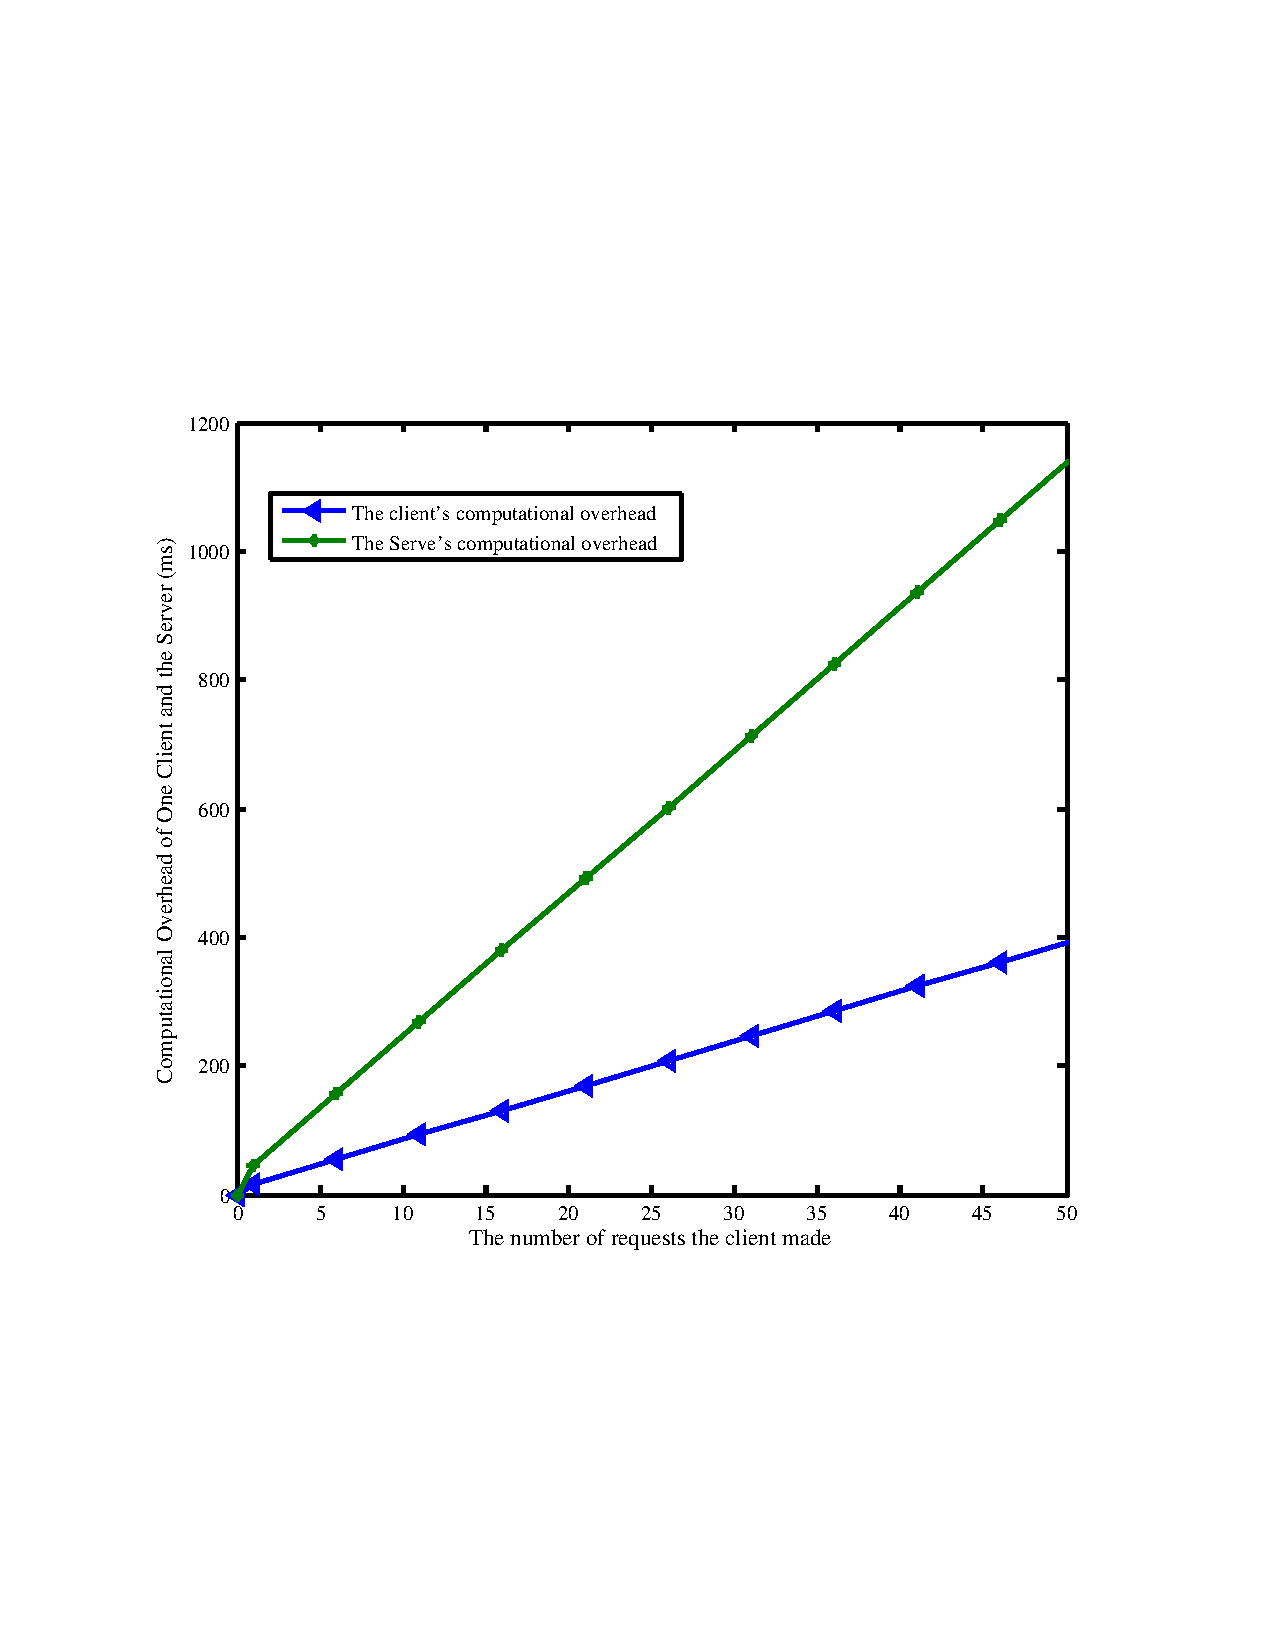
\includegraphics[width=8.0cm]{Computation_overhead_one_client}\\
  \caption{The computational overhead of one client and the server in a billing period.} \label{sec:Computationoverhead_one_Client}
\end{figure}
\begin{figure}[!htb] \centering
  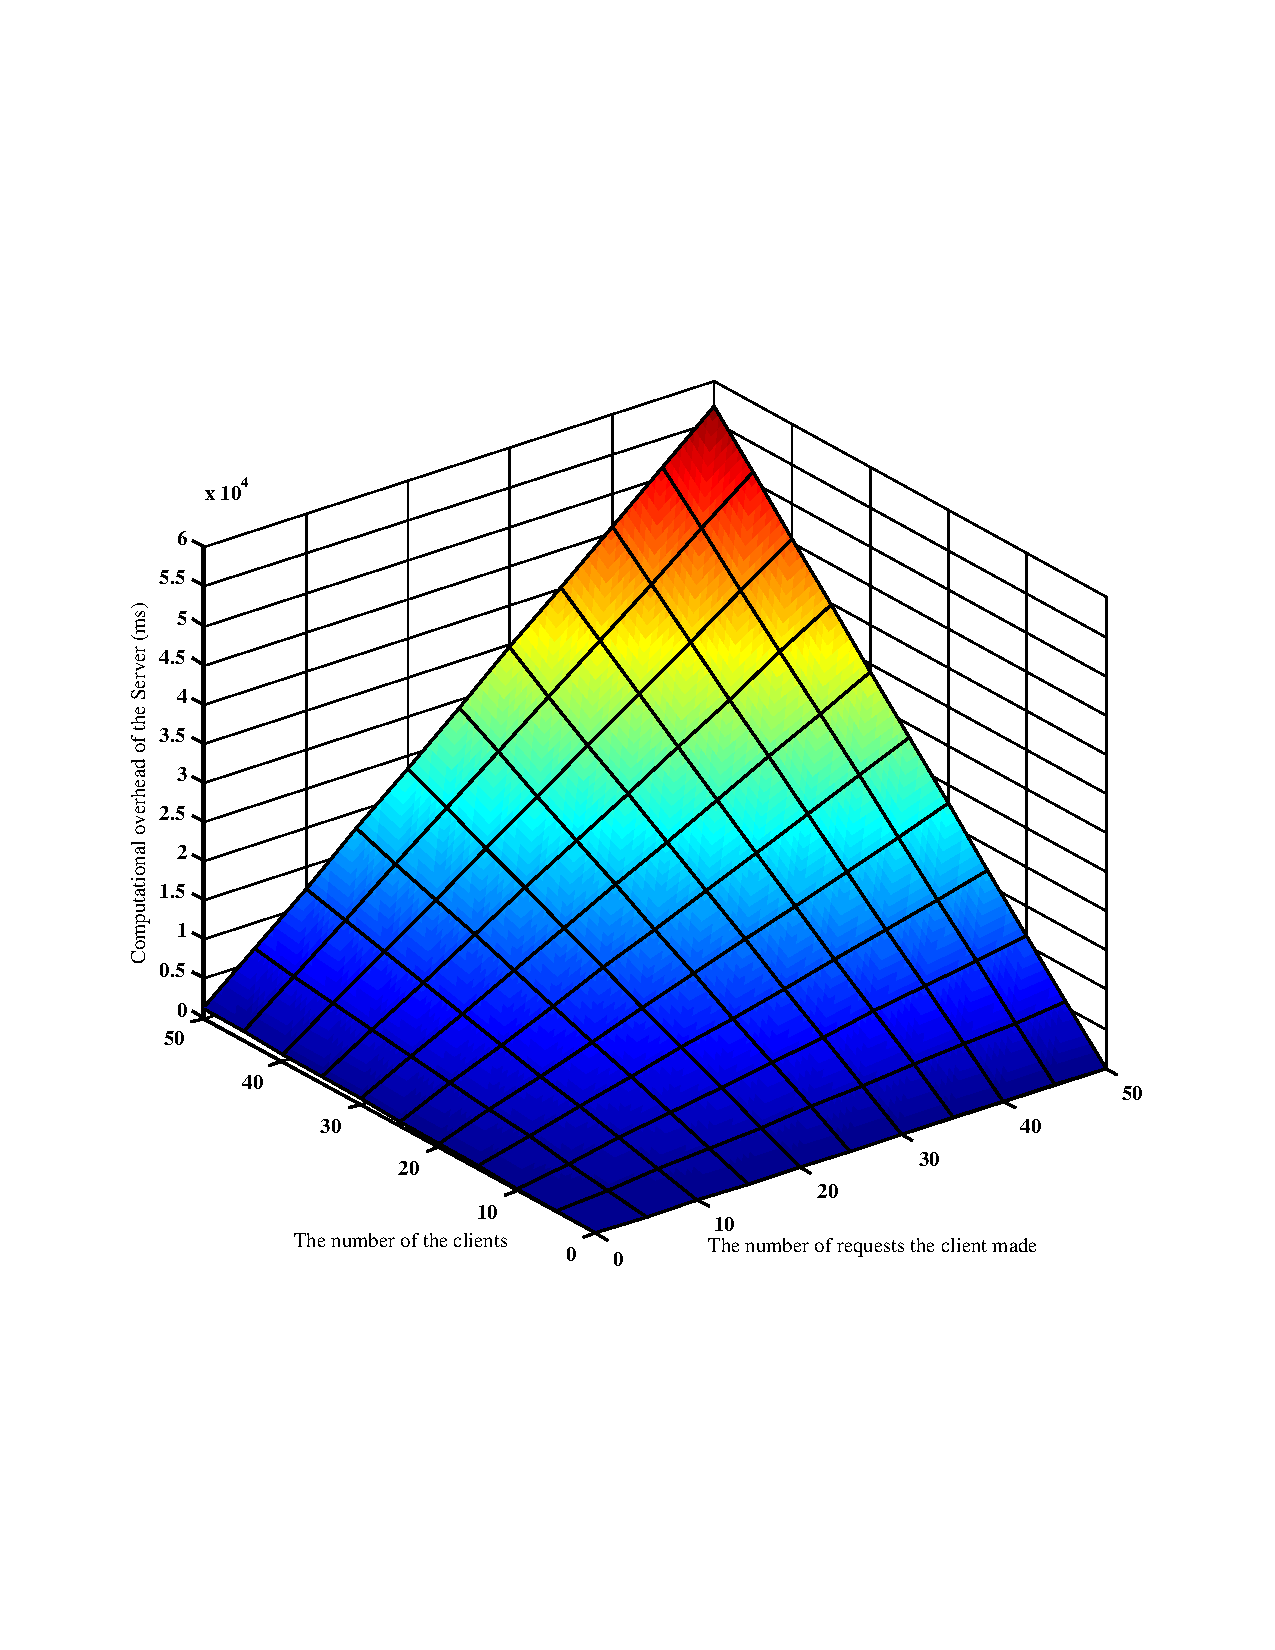
\includegraphics[width=8.0cm]{Computationoverhead_the_server}\\
  \caption{The Computational overhead of the clients in a group within one billing period.} \label{sec:Computationoverhead_the_server}
\end{figure}

\subsubsection{Communication Overhead}
We analyze the communication overhead of the proposed PPDIR scheme in terms of the public key size and the ciphertext size. Since most pairing-based cryptosystems need to work in a subgroup of an elliptic curve by representing the elliptic curve points using point compression \cite{blake2005advances}, we choose $\mathbb{G}_1$ with 160-bit order. The lengths of the elements in $\mathbb{G}_1$ and $\mathbb{G}_2$ are roughly 161-bit and 1024-bit, respectively.   Assume that the length of a hash function is 160-bit. The server needs 2048-bit to cover the length of the client's requests as each contains a number of elements including the request message, the signature, the session key, etc.

From the Setup phase in Section \ref{Sec:setup}, we know that the public key is a constant. The size of the public key can be computed from \textbf{Equation} (\ref{equa:publickeysize}). The size of the system parameters \emph{params} is $160+1024+161*3+160*3+2048=4195$-bit=525 bytes, which is computed by \eqref{equa:publickeysize}.
\begin{equation}\label{equa:publickeysize}
PK_L=|\mathbb{G}_1|+|\mathbb{G}_2|+|q|+|G|+|P|+3|H|+|n|
\end{equation}

 \begin{table*}[!htb]
\caption{Communication overhead of one Client and a group of Clients}\label{tab:Communicationoverhead:clients}
\centering
\begin{threeparttable}
\begin{tabular}{ l | c | c }
\hline
& One Client (bytes) & Group Clients (bytes)\\
\hline
Setup, Registration \&Join& $686$ & $686*N$ \\
\hline
During one  billing period& $288*m+288$ & $(288*m+288)N$ \\
\hline
\end{tabular}
 Note: $N$ is the number of group members; $m$ is the number of requests made by the client  in one billing period.
\end{threeparttable}
\end{table*}

In Section \ref{sec:sec:Registration_Join}, we notice that the client executes the Registration and Join operation only once. The size of the total exchanged messages in Registration and Join is $|rxG|+|xG|+2|rG|+|ID|+2|S_1|+|S_2|=322+966=1288$-bit, which can be explained as follow: if the client does not want to update its private key and signing key, it can continuously use its previous private key and signing key; for Registration, the client sends $rG$ to the server, and the server responses $S_1$ to the client; thus the length of the exchanged messages is $|rG|+|S_1|$, which is $161+161=322$-bit; for the Join operation, the client sends the message $\{rxG, xG, rG, ID, S_1\}$ to KGC, and KGC replies $S_2=sH_2(H(ID)||T,rxG)$ to the client; thus the length of the exchanged message is $|rxG|+|xG|+|rG|+|ID|+|S_1|+|S_2|$, which is $161*3+161*3=966$-bit.

In the Group Signature and Encryption phases, the client encrypts the signature and the original request message via Rabin Encryption; thus the length of the signed and encrypted message equals the length of the public key $n$, which is 2048-bit. At the server side, the server encrypts the response $RoR$ via AES block cipher, which needs one 256-bit block AES.  At the end of the current billing period, the client releases its token $\tau$ and the initial seed $h^0$ to the server, and  the length of the encrypted released message is 2048-bit. When the server obtains the token $\tau$ and the initial seed $h^0$,  it needs to compute the bill, and sends the bill to the clients. The server needs one block AES (256 bit) to encrypt the bill.  Thus the total message size is $2048+256=2304$-bit=288 bytes.


In Table \ref{tab:Communicationoverhead:clients}, we assume that there are $N$ clients in the group. Each client makes $n_r$ requests with the server during one billing period. Note that a client only needs to run Registration and Join Protocol once to register into the system. The communication overhead of this phase is $4195+1288=5483$-bit, which is about 686 bytes. During one billing period, the total communication overhead for a client is $(2304*n_r+2304)$ bits $=(288*n_r+288)$ bytes. For a group of $N$ clients, the communication overhead to register and join the group is $686*N$ bytes, which can be ignored as the Registration and Join operation is performed only once for each client. Therefore the total communication overhead of the group during one billing period is $(288*n_r+288)*N$.

%
\begin{figure}[!htb] \centering
  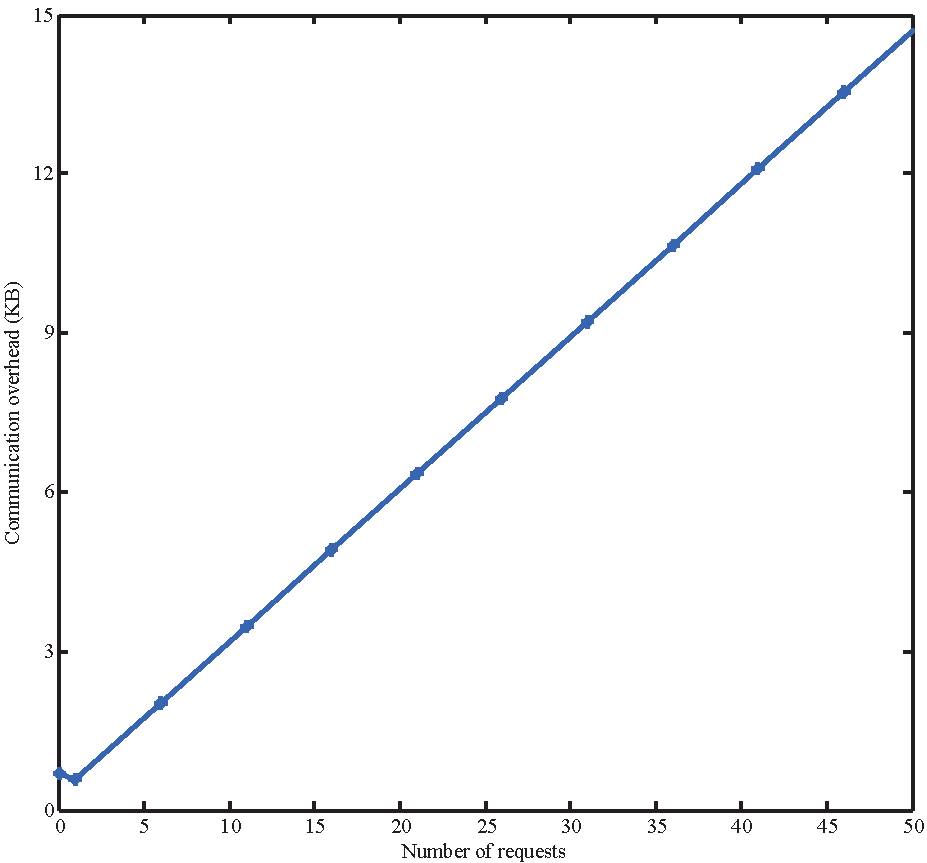
\includegraphics[width=8.0cm]{Communicationoverhead_Client}\\
  \caption{The communication overhead of one client in a billing period.} \label{sec:Communicationoverhead_Client}
\end{figure}
%
\begin{figure}[!htb] \centering
  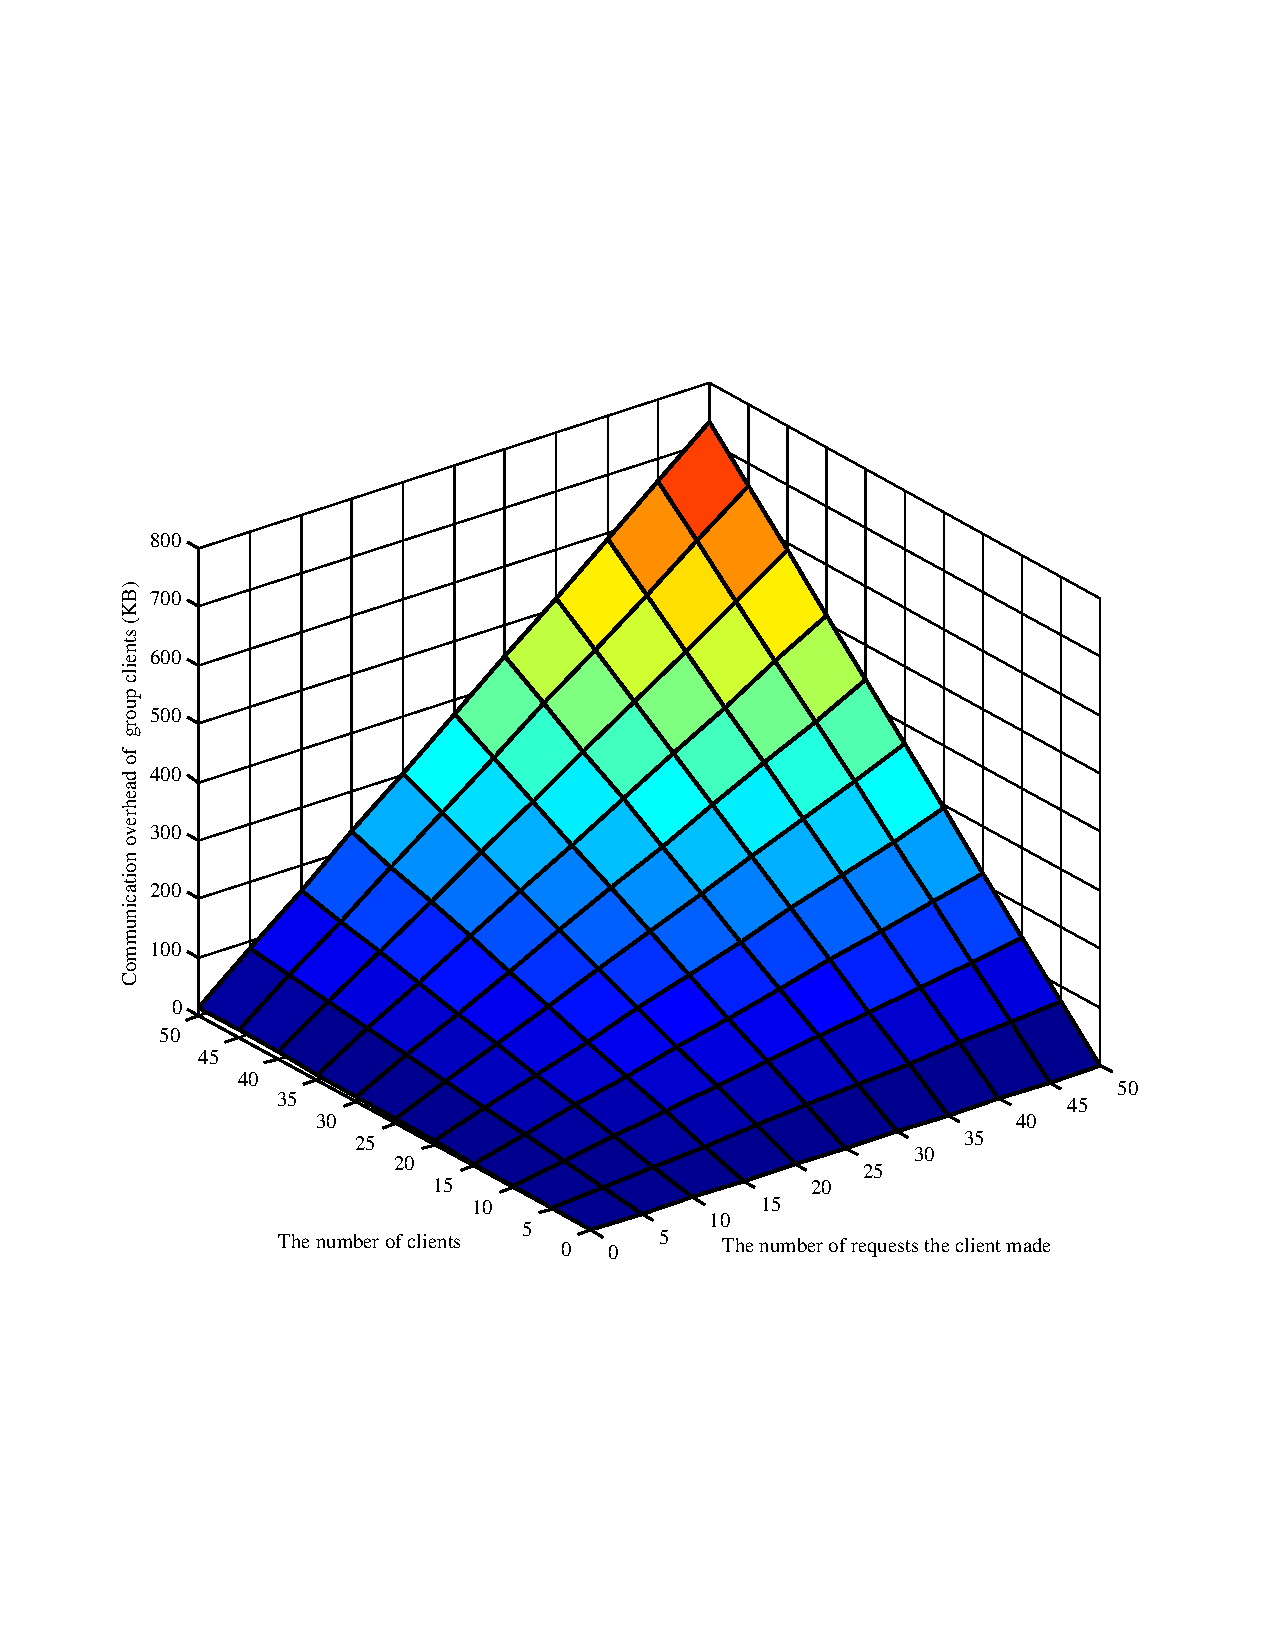
\includegraphics[width=8.0cm]{Communicationoverhead_Group_Clients}\\
  \caption{The communication overhead of a group of clients in a billing period.} \label{sec:Communicationoverhead__group_Client}
\end{figure}
%
Fig.~\ref{sec:Communicationoverhead_Client} demonstrates the communication overhead of one client in a billing period. One can see that the communication overhead increases linearly with the number of requests made. Fig.~\ref{sec:Communicationoverhead__group_Client} illustrates the communication overhead of a group of clients. We observe that the communication overhead increases with the number of clients and the number of requests made by each client.




%==========================================================================================================================
\subsection{Conclusion and Future Work}\label{sec:conclusion}

In this section, we first propose a new group signature mechanism to meet the requirements of our PPDIR scheme, and then present a privacy preservation scheme via delayed information release to protect applications that take the client-server architecture and involve billing service. Our scheme explores efficient cryptographic primitives to achieve privacy preservation. We also prove the security properties of the proposed group signature scheme and analyze the security strength of our PPDIR scheme by investigating how PPDIR can achieve privacy-preservation, non-repudiation, accountability and so on. We evaluate the performance of PPDIR in terms of communication overhead and computational overhead.

Our future research will focus on the following two directions. First, we intend to instantiate our PPDIR scheme for specific applications that require not only fine-grained privacy-preserving data collection but also other application-specific demands (such as balance checking in credit card payment), and further reduce the computational overhead and communication overhead at the client side. Second, we plan to consider the properties of secure multiparty computation, based on which to design privacy-preserving schemes without a trusted third party such that the scheme can be more suitable for practical applications.
      Our objective is to significantly reduce the query cost of node sampling over an online social network by (nearly) eliminating the costly waiting process (mixing time). Of course, as one can see from the above discussions, if we do not wait for the convergence to stationary distribution, we must somehow estimate the probability for our short walk to take a node as a sample (i.e., the node's {\em sampling probability}) before we can use the node as a sample. This is exactly what we do - i.e., we introduce a novel idea of having a (much) shorter, say $t$-step, walk, before taking a node $v$ as a sample candidate, but follow it up with a {\em proactive} process which estimates $v$'s sampling probability $p_t(v)$ - i.e., the probability for our walk to reach node $v$ at Step $t$, so that we can then use acceptance-rejection sampling to ``correct'' the sampling probability to the desired distribution. As we shall prove in the section, even though the acceptance-rejection step introduces additional query cost, the savings from having a shorter walk in the first place far outweighs the additional cost, leading to a significantly more efficient sampling process.

      Based on this idea, we develop Algorithm WALK-ESTIMATE. The algorithm takes as input a random walk based MCMC sampler, and produces samples according to the exact same distribution as the input sampler - i.e., the stationary distribution of the MCMC process. One can see that this design makes WALK-ESTIMATE transparent to the desired target distribution, making it a swap-in replacement for any random walk sampler being used (e.g., simple random walk \cite{Lovasz1993,Levin:2008}, Metropolis-Hastings random walk \cite{Lovasz1993,Levin:2008}.  As we shall demonstrate through theoretical analysis and experimental evaluation over real-world social networks, while the proactive probability-estimation process may consume a small number of queries, the significant savings from the shorter walk more than offset the additional consumption, and lead to a much more efficient sampling process over online social networks.


   \newpage
   \begin{singlespace}
   \section{Future Research Plan}
   \end{singlespace}
          \subsection{Motivation}

Suppose volunteers would like to offer their genomic data for research, as long as a strong privacy policy can be enforced without having to trust individual researchers. We remark that beyond being an illustrative example for us, abuse of sensitive data by researchers who ignore or are unaware of the limits set by the data owner is in fact a real problem, as evidenced by the case of the Havasupai tribe against the Arizona State University \cite{Tribe:Online,Havasupai:Online }. In 1989, researchers from Arizona State University partnered with the Havasupai Tribe a community with high rates of Type II Diabetes, to study links between genes and diabetes risk. When the researchers were not successful in finding a genetic link, they used the DNA from blood samples for other unrelated studies such as schizophrenia, migration, and inbreeding, all of which are taboo topics for the Havasupai \cite{Havasupai:Online}. Such unfortunate incidents can be avoided if researchers do not have direct access to this data, but can only carry out computations on this data that are subject to restrictions specified by the data owners. The restriction can include a limit on the total amount of information (number of bits) revealed to the researchers by a contributed piece of data over its life-time, a restriction on the kind of functions that can be computed on the contributed data or a requirement that certain amount of noise be added to any information computed from this data, a restriction on the number or class of researchers who can access it, etc. On the other hand, the researchers are typically not willing to publicly reveal the specific functions they are interested in. Solving this problem satisfactorily for all parties calls for leveraging tools from modern cryptography.

           \subsection{advance privacy preservation scheme based on Functional Encryption. (2015) }

           Compared with the traditional privacy preservation schemes, we want to include several extensions in our future works.
           \begin{enumerate}
               \item Explore the concept of functional encryption.
               \item Design new functional encryption for special cases. For example, in e-healthcare system, how to design the practical functional encryption to protect the patient's medicare records.
               \item Prove our scheme from different angles: security properties, computational overhead and communication overhead.
            \end{enumerate}

        \newpage
   \bibliographystyle{abbrv}
   \bibliography{proposal}
\end{document} 